\documentclass[a4paper,12pt,oneside]{book}
%\documentclass[a4paper,12pt,twoside,openright]{book}

\usepackage[utf8]{inputenc}

\usepackage[T1]{fontenc}
\usepackage[full]{textcomp}

%-------------------------------------------------------------------------------------
% MathTime Professional 2

\usepackage{newtxtext} % set Times as the default text font

% The following loads mtpro and defines some common MTPro options [2, 4]

\usepackage[complete,%
   subscriptcorrection,slantedGreek,nofontinfo,%
   mtpcal,mtpscr,% mtpluscal,%mtpcal,%
   mtphrd]{mtpro2}

%% see mtp2.tex

% Options for blackboard bold fonts [2.9]:
%   mtphrb - holey roman bold        mtpbb - blackboard bold
%   mtphrd - holey roman bold dark   mtpbbd - blackboard bold dark
%   mtphbi - holey bold italic       mtpbbi - blackboard bold italic

% Options for alternate character sets [2.6, 2.7]:
%   mtpcal - assigns Math Script to the math alphabets \mathcal and \mathbcal,
%   overwriting the default math calligraphic typeface
%   mtpccal - assigns Math Curly to the math alphabets \mathcal and \mathbcal,
%   overwriting the default math calligraphic typeface
%   mtpscr - assigns Math Script to the new math alphabets \mathscr and \mathbscr,
%       leaving \mathcal unchanged
%   mtpfrak - assigns Math Fraktur to a new math alphabet \mathfrak

% Options for AMS symbols
%   amssymbols - makes the mtpro2 AMS symbols available

% Optionally load the following package to use heavy symbols in place of bold symbols
%\usepackage{bm}

%----------------------------------------------------------------------
% font for Aspect Ratio

%\usepackage{ar}% original package by Claudio Beccari (based on Computer Modern Roman)
\usepackage[TM]{ar}% AR ligature based on Times font design
%\newcommand{\AR}{{\ARtm}}
%\newcommand{\ARb}{{\ARtmb}}




\usepackage[english,italian]{babel}
\usepackage{csquotes}
\usepackage{indentfirst}    % per avere líndentazione prima dei capitoli
\usepackage{geometry}
\geometry{a4paper, top=20mm, bottom=15mm, left=35mm, right=20mm }
\raggedbottom  % per non riempire tutta la pagina stirando il testo. puo lasciare spazi vuoti alla fine di una pagina
\linespread{1} 

\usepackage[usenames,dvipsnames]{xcolor}
\usepackage{pgfplots}
\usepackage{caption}
\usepackage{graphicx}
\usepackage{tabularx}
\usepackage{longtable}
\usepackage{multicol}
\usepackage{multirow}
\usepackage{setspace}
\usepackage{booktabs}

% \usepackage{amsmath}
%----------------------------------------------------------------------
% math

\usepackage[intlimits]{mathtools}

\usepackage{siunitx}
\usepackage{subfig}
\usepackage{rotating}
\usepackage{float}
\usepackage{fancyhdr}
\usepackage{floatflt}
\usepackage{xcolor}
\usepackage{colortbl}
\usepackage{wrapfig}
\usepackage{lipsum}
\usepackage[nouppercase, swapnames]{frontespizio}
\usepackage{adjustbox}
\usepackage{booktabs}
\usepackage{amsmath}
\usepackage{cancel}
\usepackage{listings}
\usepackage{lipsum}
\usepackage{courier}
\usepackage{xcolor}
\usepackage{relsize}
\usepackage{titlesec} 
\usepackage{appendix}
\usepackage{biblatex}
\usepackage{xspace}
    
%------------------------------------------------------------------------------------------
% LOCAL USER-DEFINED MACROS & SETTINGS
%------------------------------------------------------------------------------------------

%******************************************************************************************
%
% AUTHOR:           Agostino De Marco
% DESCRIPTION:      This is "_local_macros.tex", an auxiliary LaTeX source file.
%                   Here we collect all our user-defined macros.
%
%******************************************************************************************

%------------------------------------------------------------------------------------------
% PRE-DEFINED NAMES
%------------------------------------------------------------------------------------------



\newcommand*{\theApplicationName}{ADOpT}
\newcommand*{\theApplicationNameFull}{Aircraft Design and Optimization Tool}

\newcommand*{\OpenCascadeName}{Open CASCADE}
\newcommand*{\OpenCascadeNameFull}{\OpenCascadeName{} Technology}

%------------------------------------------------------------------------------------------
% macro per la definizione della simbologia aeronautica
%------------------------------------------------------------------------------------------

\newcommand{\Vinf}{\ensuremath{V_{\!\infty}}\xspace} % velocità asintotica
\newcommand{\vVinf}{\ensuremath{\vec{V}_{\!\!\!\infty}}\xspace} % vettore velocità asintotica

\newcommand{\Vzero}{\ensuremath{V_{\!0}}\xspace} % velocità asintotica
\newcommand{\vVzero}{\ensuremath{\vec{V}_{\mspace{-8mu}0}}\xspace} % vettore velocità asintotica

\newcommand{\Vdive}{\ensuremath{V_\text{dive}}\xspace}
\newcommand{\Vcruise}{\ensuremath{V_\text{cruise}}\xspace}

% Often used sub/superscripts
% packages amsmath & mathtools are needed

\newcommand{\Aero}{\ensuremath{\text{%
  %\mdseries\scshape a%
  A%
  }}}
\newcommand{\Thrust}{\ensuremath{\text{%
  %\mdseries\scshape t%
  T%
  }}}
\newcommand{\Grav}{\ensuremath{\text{%
  %\mdseries\scshape g%
  G%
  }}}
\newcommand{\earth}{\ensuremath{\text{%
  %\mdseries\scshape e%
  E%
  }}}% \Earth is defined elsewhere
\newcommand{\CMass}{\ensuremath{\text{%
  %\mdseries\scshape cm
  cm%
  }}}
\newcommand{\Body}{\ensuremath{\text{%
  %\mdseries\scshape b%
  B%
  }}}
\newcommand{\Fuselage}{\ensuremath{\text{%
  %\mdseries\scshape f
  F%
  }}}
\newcommand{\Wing}{\ensuremath{\text{%
   %\mdseries\scshape w%
   W%
   }}}
\newcommand{\Canard}{\ensuremath{\text{%
  %\mdseries\scshape c
  C%
  }}}
\newcommand{\Vertical}{\ensuremath{\text{%
  %\mdseries\scshape v%
  V%
  }}}
\newcommand{\VerticalI}{\ensuremath{\text{%
  %\mdseries\scshape i%
  I%
  }}}
\newcommand{\Inertial}{\ensuremath{\text{%
  %\mdseries\scshape i%
  I%
  }}}
\newcommand{\Interference}{\ensuremath{\text{%
  %\mdseries\scshape i%
  I%
  }}}

\newcommand{\Wind}{\ensuremath{\text{%
  %\mdseries\scshape w%
  wind%
  }}}
\newcommand{\Stability}{\ensuremath{\text{%
  %\mdseries\scshape s%
  S%
  }}}

\newcommand{\Stab}{\ensuremath{\mathrm{S}}}

\newcommand{\Constr}{\ensuremath{\text{
  %\mdseries\scshape c%
  C%
  }}}

\newcommand{\SeaLevel}{\ensuremath{\text{
  %\mdseries\scshape sl%
  SL%
  }}}
\newcommand{\GroundTrack}{\ensuremath{\text{%
  %\mdseries\scshape gt%
  GT%
  }}}

\newcommand{\elev}{\mathrm{e}}
\newcommand{\rud}{\mathrm{r}}
\newcommand{\ail}{\mathrm{a}}
\newcommand{\stab}{\mathrm{s}}
\newcommand{\Htail}{\ensuremath{\text{%
  %\mdseries\scshape h%
  H%
  }}}
\newcommand{\Vtail}{\ensuremath{\text{%
  %\mdseries\scshape v%
  V%
  }}}
\newcommand{\flap}{\mathrm{f}}
\newcommand{\tab}{\mathrm{t}}

% Mach and Reynolds numbers
\newcommand{\Mach}{\ensuremath{M}\xspace}%
\newcommand{\Reynolds}{\ensuremath{\mathit{Re}}\xspace}

\newcommand{\deltaE}{\ensuremath{\delta_\elev}\xspace}
\newcommand{\deltaA}{\ensuremath{\delta_\ail}\xspace}
\newcommand{\deltaR}{\ensuremath{\delta_\rud}\xspace}
\newcommand{\deltaS}{\ensuremath{\delta_\stab}\xspace}


\newcommand{\Cbarbar}{\ensuremath{%
%\substack{=\\{\displaystyle c}}}
\begin{array}[b]{@{}c@{}}\mathsmaller{=}\\[-1.6ex]c\end{array}
%\bar{\bar{c}}%
%
% http://groups.google.it/group/comp.text.tex/browse_thread/thread/420529a68269d791/587ffe9ccc433d86?lnk=raot
%
}\xspace} % m.a.c. ESDU style

\newcommand{\mmtow}{\ensuremath{m_\text{MTO}}\xspace}
\newcommand{\wmtow}{\ensuremath{W_\text{MTO}}\xspace}
\newcommand{\mmzfw}{\ensuremath{m_\text{MZF}}\xspace}
\newcommand{\wmzfw}{\ensuremath{W_\text{MZF}}\xspace}
\newcommand{\mml}{\ensuremath{m_\text{ML}}\xspace}
\newcommand{\wml}{\ensuremath{W_\text{ML}}\xspace}

\newcommand{\Cbar}{\ensuremath{\bar{c}}\xspace} % m.a.c.
\newcommand{\CG}{CG}
\newcommand{\Scs}{\ensuremath{S_\text{cs}}\xspace}
\newcommand{\tc}{\ensuremath{(t/c)}\xspace}
\newcommand{\tcroot}{\ensuremath{(t/c)_\text{r}}\xspace}
\newcommand{\tcmean}{\ensuremath{\xbar{(t/c)}}\xspace}
\newcommand{\alphazeroL}{\ensuremath{\alpha_{{0L}}}\xspace}
\newcommand{\epsg}{\ensuremath{\varepsilon}_\mathrm{g}\xspace} %Angolo di svergolamento geometrico dell'ala
\newcommand{\xcg}{\ensuremath{{x}_{\text{cg}}}} % posizione adimesionale del baricentro
\newcommand{\xQC}{\ensuremath{x_{c/4}\xspace}} % posizione adimesionale del baricentro
\newcommand{\xac}{\ensuremath{\ensuremath{{x}_\mathrm{ac}}}} % posizione adimensionale del c.a.
\newcommand{\xLE}{\ensuremath{{x}_{\text{LE}}\xspace}}
\newcommand{\xTE}{\ensuremath{{x}_{\text{TE}}\xspace}}
\newcommand{\yLE}{\ensuremath{{y}_{\text{LE}}\xspace}}
\newcommand{\yTE}{\ensuremath{{y}_{\text{TE}}\xspace}}
\newcommand{\xN}{\ensuremath{\hat{x}_{\text{N}}}} % posizione adimesionale del punto neutro

\newcommand{\CLiftW}{\ensuremath{C_{L_{\mathrm{W}}}}\xspace} %Coefficiente di portanza dell'ala
\newcommand{\CLzeroW}{\ensuremath{C_{L_{0 \mathrm{,W}}}}\xspace} %CL dell'ala a portanza nulla
\newcommand{\ClalphapW}{\ensuremath{\big(C_{l_{\mathlarger\alpha}}\big)_{\mathrm{Profilo},\mathrm{W}}}\xspace} %Clalfa 2D
\newcommand{\CLalphaW}{\ensuremath{C_{L_{\mathlarger{\alpha}\mathrm{,W}}}}\xspace} %gradiente della retta di portanza dell'ala
\newcommand{\CLalphaWclassic}{\ensuremath{C_{L_{\mathlarger{\alpha}\mathrm{,W \mathit{,classic}}}}}\xspace} %gradiente della retta di portanza dell'ala calcolato con formula classica

\newcommand{\CMac}{\ensuremath{C_{\mathcal{M}_{\mathrm{ac}}}}\xspace} %Coeff di momento totale rispetto al centro aerodinamico dell'ala
\newcommand{\CMCGW}{\ensuremath{C_{\mathcal{M}_\mathrm{CG,W}}}\xspace} %Coeff. di momento rispetto al baricentro, contributo dell'ala
\newcommand{\CMzeroW}{\ensuremath{C_{\mathcal{M}_{0,\mathrm{W}}}}\xspace} %coefficiente di momento a portanza nulla
\newcommand{\CMalphaW}{\ensuremath{\big(C_{\mathcal{M}\alpha}\big)_\mathrm{W}}\xspace} %coefficiente di momento a portanza nulla
\newcommand{\CMacWRoskam}{\ensuremath{C_{\mathcal{M}_{\mathrm{ac,W}_\mathit{Roskam}}}}\xspace} %Coeff di momento rispetto al centro aerodinamico con la formula di Roskam

\newcommand{\xacW}{\ensuremath{\ensuremath{\big(\hat{x}_{ac}\big)_\mathrm{W}}}\xspace} %posizione adimensionale del c.a. dell'ala
\newcommand{\alphazlr}{\ensuremath{\alpha_{{0L}_{\mathrm{\larger root}}}}\xspace} %angolo di portaza nulla alla radice
\newcommand{\alphazlt}{\ensuremath{\alpha_{{0L}_{\mathrm{\larger tip}}}}\xspace} %angolo di portaza nulla alla estremità
\newcommand{\alphazeroLW}{\ensuremath{\alpha_{{0L},\mathrm{W}}}\xspace} %angolo di portanza nulla dell'ala
\newcommand{\alphazlpW}{\ensuremath{\alpha_{{0L}_{\mathrm{\larger Profilo}}}}\xspace} %angolo di portanza nulla del profilo dell'ala
\newcommand{\epstip}{\ensuremath{\epsilon_{\mathrm{tip}}}\xspace} %svergolamento all'estremità

\newcommand{\frecciaLE}{\ensuremath{\Lambda_{\mathrm{leading edge}}}\xspace} %freccia del bordo di attacco
\newcommand{\frecciaTE}{\ensuremath{\Lambda_{\mathrm{trailing edge}}}\xspace} %frecica del bordo di uscita
\newcommand{\LambdaLE}{\ensuremath{\Lambda_{\mathit{LE}}}\xspace} %freccia del bordo di attacco
\newcommand{\LambdaTE}{\ensuremath{\Lambda_{\mathrm{t.e.}}}\xspace} %freccia del bordo di uscita
\newcommand{\LambdaQC}{\ensuremath{\Lambda_{c/4}}\xspace} %freccia del bordo di attacco quarter chord
\newcommand{\LambdaHC}{\ensuremath{\Lambda_{c/2}}\xspace} %freccia del bordo di attacco half chord
\newcommand{\LambdaN}{\ensuremath{\Lambda_{n}}\xspace} %freccia del bordo di uscita
\newcommand{\Lambdax}{\ensuremath{\Lambda_{\mathit{x}}}\xspace} %freccia ad una generica percentuale x della corda
\newcommand{\LambdaEA}{\ensuremath{\Lambda_\mathrm{ea}}\xspace} % freccia dell'asse elastico
\newcommand{\Lambdatmax}{\ensuremath{\Lambda_{\mathit{t}_\mathit{max}}}\xspace} %freccia nel punto di maggior spessore relativo
\newcommand{\GammaW}{\ensuremath{\Gamma_{\mathrm{W}}}\xspace} %angolo diedro

\newcommand{\tauail}{\ensuremath{\tau_\ail}\xspace} %Efficienza degli alettoni
\newcommand{\cail}{\ensuremath{\mathlarger{c}_{\mathrm{\ail}}}\xspace} %Corda dell'alettone
\newcommand{\cflap}{\ensuremath{\mathlarger{c}_{\mathrm{\flap}}}\xspace} %Corda del flap
\newcommand{\etaailin}{\ensuremath{\mathlarger{\eta}_{\mathrm{\ail\mathit{,in}}}}\xspace} %Stazione interna degli alettoni, adim
\newcommand{\etaailout}{\ensuremath{\mathlarger{\eta}_{\mathrm{\ail\mathit{,out}}}}\xspace} %Stazione esterna degli alettoni, adim
\newcommand{\etaflapin}{\ensuremath{\mathlarger{\eta}_{\mathrm{\flap\mathit{,in}}}}\xspace} %Stazione interna dei flap, adim
\newcommand{\etaflapout}{\ensuremath{\mathlarger{\eta}_{\mathrm{\flap\mathit{,out}}}}\xspace} %Stazione esterna dei flap, dim
\newcommand{\yailin}{\ensuremath{\mathlarger{y}_{\mathrm{\ail\mathit{,in}}}}\xspace} %Stazione interna degli alettoni, dim
\newcommand{\yailout}{\ensuremath{\mathlarger{y}_{\mathrm{\ail \mathit{,out}}}}\xspace} %Stazione esterna degli alettoni, dim
\newcommand{\yflapin}{\ensuremath{\mathlarger{y}_{\mathrm{\flap\mathit{,in}}}}\xspace} %Stazione interna dei flap, adim
\newcommand{\yflapout}{\ensuremath{\mathlarger{y}_{\mathrm{\flap\mathit{,out}}}}\xspace} %Stazione esterna dei flap, dim
\newcommand{\Sail}{\ensuremath{S_{\mathrm{\ail}}}\xspace} %Superfice degli alettoni
\newcommand{\Sflap}{\ensuremath{S_{\mathrm{\flap}}}\xspace} %Superfice dei flaps
\newcommand{\alphazeroLWflap}{\ensuremath{\alpha_{{0L_{\mathrm{W} \mathit{,flap}}}}}\xspace} %angolo di portanza nulla dell'ala con flaps estesi
\newcommand{\alphazerolWflap}{\ensuremath{\alpha_{{0\ell_{\mathrm{W} \mathit{,flap}}}}}\xspace} %angolo di portanza nulla di un profilo con flap esteso

%metodo di shrenk per il carico alare
\newcommand{\cell}{\ensuremath{\mathlarger{c}_{\mathrm{ell}}}\xspace} %Corda dell'ala ellittica
\newcommand{\cellzero}{\ensuremath{\mathlarger{c}_{\mathrm{ell}_0}}\xspace} %Corda dell'ala ellittica
\newcommand{\ceff}{\ensuremath{\mathlarger{c}_{\mathrm{eff}}}\xspace} %Corda effettiva dell'ala
\newcommand{\cClbasic}{\ensuremath{\mathlarger{cC}_{\mathrm{\ell}_b}}\xspace} %Carico basico
\newcommand{\cCladd}{\ensuremath{\mathlarger{cC}_{\mathrm{\ell}_a}}\xspace} %Carico addizionale
\newcommand{\CLbasic}{\ensuremath{\mathlarger{C}_{\mathrm{L}_b}}\xspace} %Carico basico
\newcommand{\CLadd}{\ensuremath{\mathlarger{C}_{\mathrm{L}_a}}\xspace} %Carico addizionale


%fusoliera
\newcommand{\FFR}{\ensuremath{F\hspace{-0.1em}R\hspace{-0.1em}R}\xspace} %Rapporto di snellezza della fusoliera
\newcommand{\lF}{\ensuremath{{l_\mathrm{F}}}\xspace} %Lunghezza della fusoliera
\newcommand{\lFmax}{\ensuremath{{l_\mathrm{F,max}}}\xspace} %Lunghezza della fusoliera
\newcommand{\lstructF}{\ensuremath{{l_\mathrm{struc,F}}}\xspace} %Lunghezza strutturale della fusoliera
\newcommand{\dF}{\ensuremath{{d_{\mathrm{F}}}}\xspace} %Diametro della fusoliera
\newcommand{\dFmax}{\ensuremath{{d_\mathrm{F,max}}}\xspace}
\newcommand{\dFF}{\ensuremath{{{d}_{\mathrm{F}}^2(x)}}\xspace} %Diametro quadro della fusoliera
\newcommand{\hF}{\ensuremath{{{h}_{\mathrm{F}}}}\xspace} %Ampiezza della fusoliera
\newcommand{\hFmax}{\ensuremath{{{h}_{\mathrm{F,max}}}}\xspace} %Ampiezza della fusoliera
\newcommand{\wF}{\ensuremath{{{w}_{\mathrm{F}}}}\xspace} %Ampiezza della fusoliera
\newcommand{\wFmax}{\ensuremath{{{w}_{\mathrm{F,max}}}}\xspace} %Ampiezza della fusoliera
\newcommand{\wFF}{\ensuremath{{{w}_{\mathrm{F}}^2(x)}}\xspace} %Ampiezza quadra della fusoliera
\newcommand{\SFside}{\ensuremath{{S_\mathrm{F,side}}}\xspace} %Superficie di ingombro laterale della fusoliera
\newcommand{\SwetF}{\ensuremath{{S_\mathrm{wet,F}}}\xspace}
\newcommand{\diffPF}{\ensuremath{{\Delta P_\mathrm{F}}}\xspace}
\newcommand{\diffPFmax}{\ensuremath{{\Delta P_\mathrm{F,max}}}\xspace}
\newcommand{\icl}{\ensuremath{{i_\mathrm{cl}}}\xspace}

\newcommand{\MF}{\ensuremath{\mathcal{M}_{\mathrm{F}}}\xspace} %Momento rispetto al baricentro, contributo della fusoliera
\newcommand{\CMF}{\ensuremath{C_{\mathcal{M}_{\mathrm{F}}}}\xspace} %Coefficiente di momento, contributo della fusoliera
\newcommand{\CMzeroF}{\ensuremath{C_{\mathcal{M}\mathrm{_0,F}}}\xspace} 
%Coeff di momento della fusoliera ad angolo di attacco nullo
\newcommand{\CMalphaF}{\ensuremath{C_{\mathcal{M}\alpha\mathrm{,F}}}\xspace} 
%Gradiente del coefficiente di momento di beccheggio della fusoliera
\newcommand{\CNbetaF}{\ensuremath{\big(C_{\mathcal{N}_{\mathlarger{\beta}}}\big)_\mathrm{F}}\xspace} 
%Gradiente del coefficiente di momento di imbardata della fusoliera

%nacelle
\newcommand{\SwetN}{\ensuremath{{S_\mathrm{wet,N}}}\xspace}


%piano orizz. di coda
\newcommand{\CbarH}{\ensuremath{\mathlarger{\bar{c}}_{\mathrm{H}}}\xspace} %Corda media del piano di coda orizz.
\newcommand{\alphaH}{\ensuremath{\alpha_{\mathrm{H}}}\xspace} %Incidenza dle piano di coda orizz.
\newcommand{\alphaHzero}{\ensuremath{\alpha_{\mathrm{H}_0}}\xspace} %Incidenza del piano di coda orizz. quando il CL totale del velivolo è 0
\newcommand{\alphazlH}{\ensuremath{\alpha_{{0L},\mathrm{H}}}\xspace} %angolo di portanza nulla del piano orizz.
\newcommand{\iH}{\ensuremath{i_{\mathrm{H}}}\xspace} % angolo di calettamento del piano di coda
\newcommand{\qH}{\ensuremath{q_{\mathrm{H}}}\xspace} %Pressione dinamica sul piano  di coda orizz.
\newcommand{\etaH}{\ensuremath{\mathlarger{\eta}_{\mathrm{H}}}\xspace} %Rapporto tra le pressioni dinamiche sul piano orizz.
\newcommand{\SH}{\ensuremath{S_{\mathrm{H}}}\xspace} %Superficie del piano di coda orizz.
\newcommand{\cH}{\ensuremath{{c_{\mathrm{H}}}}\xspace} %Corda del piano di coda orizz.
\newcommand{\bH}{\ensuremath{{\mathlarger{b}_{\mathrm{H}}}}\xspace} %Apertura alare del piano di coda orizz.
\newcommand{\VH}{\ensuremath{\bar{\mathcal{V}}_{\mathrm{H}}}\xspace} %Rapporto volumetrico del piano orizzontale
\newcommand{\Se}{\ensuremath{S_{\elev}}\xspace} %Superficie dell' equilibratore
\newcommand{\ce}{\ensuremath{{c_{\elev}}}\xspace} %Corda dell'equilibratore
\newcommand{\eH}{\ensuremath{\mathlarger{e}_{\mathrm{H}}}\xspace} %Fattore di Oswald del piano di coda orizz.
\newcommand{\ARH}{\ensuremath{\AR_{\mathrm{H}}}\xspace} %Aspect Ratio del piano di coda orizz.
\newcommand{\lamH}{\ensuremath{\mathlarger{\lambda}_{\mathrm{H}}}\xspace} %Taper Ratio del piano orizz. (rapporto dirastremazione)

\newcommand{\CLH}{\ensuremath{C_{L_\mathrm{H}}}\xspace} %Coefficente di  portanza del piano di coda orizz.
\newcommand{\CLiftH}{\ensuremath{C_{L_{\mathrm{H}}}}\xspace} %Coefficiente di portanza sul piano di coda orizz.
\newcommand{\ClalphapH}{\ensuremath{\big(C_{l_{\mathlarger\alpha}}\big)_{\mathrm{Profilo},\mathrm{H}}}\xspace} %Clalfa 2D
\newcommand{\CLalphaH}{\ensuremath{C_{L_{\mathlarger\alpha\mathrm{,H}}}}\xspace} %Clalfa 3D
\newcommand{\epszero}{\ensuremath{\epsilon_0}\xspace} %Downwash ad alpha =0
\newcommand{\udeps}{\ensuremath{\Bigg(1-\frac{\diff{\epsilon}}{\diff{\alpha}}\Bigg)}\xspace} %(1-deps/dalpha)
\newcommand{\udepsfrac}{\ensuremath{\left(1-\mathlarger{\diff{\varepsilon}/\diff{\alpha}}\right)}\xspace} % (1-deps/dalpha)
\newcommand{\depsfrac}{\ensuremath{\frac{\diff{\varepsilon}}{\diff{\alpha}}}\xspace} %(deps/dalpha)
\newcommand{\deps}{\ensuremath{\diff{\varepsilon}/\diff{\alpha}}\xspace} %(deps/dalpha)
\newcommand{\depsshort}{\ensuremath{\mathlarger{\varepsilon}_\alpha}} %deps/dalpha notazione sintetica

\newcommand{\tauH}{\ensuremath{\mathlarger{\tau}_{\mathrm{H}}}\xspace} % efficacia del timone orizzontale
\newcommand{\tauelev}{\ensuremath{\mathlarger{\tau}_\elev}\xspace} % efficacia dell'elevatore
\newcommand{\tauequilib}{\ensuremath{\mathlarger{\tau}_{\mathrm{equilib}}}\xspace} %Efficienza del piano di coda
\newcommand{\etaelevin}{\ensuremath{\mathlarger{\eta}_{\mathrm{\elev,in}}}\xspace} %Stazione interna dell'elevatore, adim
\newcommand{\etaelevout}{\ensuremath{\mathlarger{\eta}_{\mathrm{\elev,out}}}\xspace} %Stazione esterna dell'elevatore, adim

\newcommand{\CH}{\ensuremath{C_{\mathrm{H}}}\xspace} %Forza assiale sul piano di coda orizz.
\newcommand{\CCH}{\ensuremath{C_{C_{\mathrm{H}}}}\xspace} %Coefficiente di forza assiale sul piano di coda orizz.
\newcommand{\NH}{\ensuremath{N_{\mathrm{H}}}\xspace} %Forza normale sul piano di coda orizz.
\newcommand{\CNH}{\ensuremath{C_{N_{\mathrm{H}}}}\xspace} %Coefficiente di forza normale sul piano di coda orizz.

\newcommand{\MacH}{\ensuremath{\mathcal{M}_{\mathrm{ac,H}}}\xspace} %Momento focale del piano di coda orizz.
\newcommand{\CMacH}{\ensuremath{C_{\mathcal{M}_{\mathrm{ac,H}}}}\xspace} %Coefficiente di momento focale del piano di coda orizz.

\newcommand{\Mhe}{\ensuremath{\mathcal{M}_{\mathcal{h}_{\elev}}}\xspace} %Momento di cerniera dell'equilibratore
\newcommand{\Che}{\ensuremath{C_{\mathcal{h}_{\elev}}}\xspace} %Coefficiente di momento di cerniera dell'equilibratore
\newcommand{\Cheo}{\ensuremath{C_{\mathcal{h}_{\elev 0}}}\xspace} %Coeff di mom di cerniera dell'equil ad alpha e deltae nulli
\newcommand{\Chalphae}{\ensuremath{C_{\mathcal{H}_{\alpha_{\elev}}}}\xspace} %Coeff di mom di cern dell'equil - derivata rispetto ad alpha
\newcommand{\Chdeltae}{\ensuremath{C_{\mathcal{H}_{\delta_{\elev}}}}\xspace} %Coeff di mom di cern dell'equil - derivata rispetto a delta
\newcommand{\Chdeltat}{\ensuremath{C_{\mathcal{h}_{\delta_\mathrm{t}}}}\xspace} 
%Coeff di mom di cern dell'equil - derivata rispetto a deltat
\newcommand{\deltaef}{\ensuremath{\delta_{\elev_{\mathrm{f}}}}\xspace} %Angolo di flottaggio dell'equilibratore
\newcommand{\deltat}{\ensuremath{\delta_{\mathrm{t}}}\xspace} %Angolo di deflessione del trim tab

\newcommand{\LHe}{\ensuremath{{L_{\mathrm{He}}}}\xspace} %Carico di equilibrio sul piano di coda
\newcommand{\deltaEo}{\ensuremath{{\delta_{\elev\mathrm{0}}}}\xspace} %Deflessione dell'equilibratore necessaria all'equilibrio a CL=0
\newcommand{\deltaEe}{\ensuremath{{\delta_{\elev\mathrm{e}}}}\xspace} 
%Deflessione dell'equilibratore necessaria all'equilibrio a CL generico
\newcommand{\deltaEmax}{\ensuremath{{\delta_{\elev_{\mathrm{max}}}}}\xspace} 
%Deflessione dell'equilibratore necessaria all'equilibrio a CLmax
\newcommand{\deltae}{\ensuremath{{\delta_{\elev}}}\xspace} 
%Deflessione dell'equilibratore necessaria all'equilibrio a CL generico


%piano vert. di coda
\newcommand{\CbarV}{\ensuremath{\mathlarger{\bar{c}}_{\mathrm{V}}}\xspace} %Corda media del piano di coda vert.
\newcommand{\alphazlV}{\ensuremath{\alpha_{{0L},\mathrm{V}}}\xspace} %angolo di portanza nulla del piano vert.
\newcommand{\qV}{\ensuremath{q_{\mathrm{V}}}\xspace} %Pressione dinamica sul piano  di coda vert.
\newcommand{\etaV}{\ensuremath{\mathlarger{\eta}_{\mathrm{V}}}\xspace} %Rapporto tra le pressioni dinamiche sul piano vert.
\newcommand{\SV}{\ensuremath{S_{\mathrm{V}}}\xspace} %Superficie del piano di coda vert.
\newcommand{\cV}{\ensuremath{{c_{\mathrm{V}}}}\xspace} %Corda del piano di coda vert.
\newcommand{\bV}{\ensuremath{{b_{\mathrm{V}}}}\xspace} %''Apertura alare'' del piano di coda vert.
\newcommand{\VV}{\ensuremath{\bar{\mathcal{V}}_{\mathrm{V}}}\xspace} %Rapporto volumetrico del piano orizzontale
\newcommand{\Srud}{\ensuremath{S_{\rud}}\xspace} %Superficie del timone
\newcommand{\crud}{\ensuremath{{c_{\rud}}}\xspace} %Corda del timone
\newcommand{\eV}{\ensuremath{\mathlarger{e}_{\mathrm{V}}}\xspace} %Fattore di Oswald del piano di coda vert.
\newcommand{\ARV}{\ensuremath{\AR_{\mathrm{V}}}\xspace} %Aspect Ratio del piano di coda vert.
\newcommand{\lamV}{\ensuremath{\mathlarger{\lambda}_{\mathrm{V}}}\xspace} %Taper Ratio del piano vert. (rapporto dirastremazione)

\newcommand{\CLiftV}{\ensuremath{C_{L_{\mathrm{H}}}}\xspace} %Coefficiente di portanza sul piano di coda vert.
\newcommand{\ClalphapV}{\ensuremath{\big(C_{l_{\mathlarger\alpha}}\big)_{\mathrm{Profilo},\mathrm{V}}}\xspace} %Clalfa 2D
\newcommand{\CLalphaV}{\ensuremath{C_{L_{\mathlarger\alpha\mathrm{,V}}}}\xspace} %Clalfa 3D
\newcommand{\sidewash}{\ensuremath{\displaystyle\frac{\diff{\sigma}}{\diff{\beta}}}} %Sidewash

\newcommand{\MacV}{\ensuremath{\mathcal{M}_{\mathrm{ac,V}}}\xspace} %Momento focale del piano di coda vert.
\newcommand{\CMacV}{\ensuremath{C_{\mathcal{M}_{\mathrm{ac,V}}}}\xspace} %Coefficiente di momento focale del piano di coda vert.

\newcommand{\taurud}{\ensuremath{\mathlarger{\tau}_\rud}\xspace} % efficacia del timone
\newcommand{\etarudin}{\ensuremath{\mathlarger{\eta}_{\mathrm{\rud,in}}}\xspace} %Stazione interna del timone, adim
\newcommand{\etarudout}{\ensuremath{\mathlarger{\eta}_{\mathrm{\rud,out}}}\xspace} %Stazione esterna del timone, adim


%assi e forze di natura aerodinamica
\newcommand{\XA}{\ensuremath{X_\Aero}\xspace}
\newcommand{\YA}{\ensuremath{Y_\Aero}\xspace}
\newcommand{\ZA}{\ensuremath{Z_\Aero}\xspace}
\newcommand{\LA}{\ensuremath{\mathcal{L}_\Aero}\xspace}
\newcommand{\MA}{\ensuremath{\mathcal{M}_\Aero}\xspace}
\newcommand{\NA}{\ensuremath{\mathcal{N}_\Aero}\xspace}


%configurazioni degli assemblaggi delle parti del velivolo
\newcommand{\BVH}{\ensuremath{\mathrm{BVH}}\xspace}
\newcommand{\WB}{\ensuremath{\mathrm{WB}}\xspace}
\newcommand{\WiB}{\ensuremath{\mathrm{W(B)}}\xspace}
\newcommand{\BiW}{\ensuremath{\mathrm{B(W)}}\xspace}
\newcommand{\WBV}{\ensuremath{\mathrm{WBV}}\xspace}
\newcommand{\WBH}{\ensuremath{\mathrm{WBH}}\xspace}
\newcommand{\Nose}{\ensuremath{\mathrm{N}}\xspace}
\newcommand{\HiB}{\ensuremath{\mathrm{H(B)}}\xspace}
\newcommand{\BiH}{\ensuremath{\mathrm{B(H)}}\xspace}


%Altre distanze tra baricentri e centri aerodinamici
\newcommand{\xcgdim}{\ensuremath{\mathlarger{x}_{\mathrm{CG}}}\xspace} %Posizione longitudinale baricentro sulla corda dell'ala - dimensionale
\newcommand{\xacdim}{\ensuremath{\mathlarger{x}_{\mathrm{AC}}}\xspace} %Posizione longitudinale c.a. sulla corda dell'ala - dimensionale
\newcommand{\xicgadim}{\ensuremath{\mathlarger{\xi}_{\mathrm{CG}}}\xspace} %Posizione longitudinale baricentro sulla corda dell'ala - adimensionale
\newcommand{\xiacadim}{\ensuremath{\mathlarger{\xi}_{\mathrm{AC}}}\xspace} %Posizione longitudinale c.a. sulla corda dell'ala - adimensionale
\newcommand{\xiacadimWB}{\ensuremath{\mathlarger{\xi}_{\mathrm{AC \mathrm{,WB}}}}\xspace} %Posizione longitudinale c.a. sulla corda dell'ala - adimensionale
\newcommand{\xiacadimW}{\ensuremath{\mathlarger{\xi}_{\mathrm{AC \mathrm{,W}}}}\xspace} %Posizione longitudinale c.a. sulla corda dell'ala - adimensionale
\newcommand{\xiacadimH}{\ensuremath{\mathlarger{\xi}_{\mathrm{AC \mathrm{,H}}}}\xspace} %Posizione longitudinale c.a. sulla corda dell'ala - adimensionale
\newcommand{\xNdim}{\ensuremath{\mathlarger{x}_{\mathrm{N}}}\xspace} %Posizione longitudinale del punto neutro sulla corda dell'ala - dimensionale
\newcommand{\xiNadim}{\ensuremath{\mathlarger{\xi}_{\mathrm{N}}}\xspace} %Posizione longitudinale del punto neutro sulla corda dell'ala - adimensionale
\newcommand{\xiNadimfree}{\ensuremath{\mathlarger{\xi}_{\mathrm{N_\mathit{free}}}}\xspace} %Posizione longitudinale del punto neutro sulla corda dell'ala - adimensionale
\newcommand{\xiNadimeng}{\ensuremath{\mathlarger{\xi}_{\mathrm{N_\mathit{eng}}}}\xspace} %Posizione longitudinale del punto neutro sulla corda dell'ala - adimensionale - considerando i motori
\newcommand{\deltaxiNadimeng}{\ensuremath{\mathlarger{\Delta\xi}_{\mathrm{N_\mathit{eng}}}}\xspace} %Posizione longitudinale del punto neutro sulla corda dell'ala - adimensionale - considerando i motori
\newcommand{\xNCLdim}{\ensuremath{x_{\mathrm{N}^{\prime}}}\xspace} %Pos. longit. del punto neutro a C.L. sulla corda dell'ala - dimensionale
\newcommand{\xacwdim}{\ensuremath{x_{{\mathrm{ac}}_w}}\xspace} %Posizione longitudinale c.a. sulla corda dell'ala - dimensionale
\newcommand{\xacdimh}{\ensuremath{\mathlarger{x}_{\mathrm{AC \mathrm{,H}}}}\xspace} %Posizione longitudinale c.a. sulla corda dell'ala - dimensional
\newcommand{\xa}{\ensuremath{x_{\mathrm{a}}}\xspace} %Distanza longitudinale baricentro-c.a. dell'ala
\newcommand{\za}{\ensuremath{z_{\mathrm{a}}}\xspace} %Distanza verticale baricentro-c.a. dell'ala
\newcommand{\lH}{\ensuremath{\ell_{\mathrm{H}}}\xspace} %Distanza longitudinale baricentro-c.a. del piano di coda orizz.
\newcommand{\hH}{\ensuremath{h_{\mathrm{H}}}\xspace} %Distanza verticle baricentro-c.a. del piano di coda orizz.
\newcommand{\zH}{\ensuremath{z_{\mathrm{H}}}\xspace} %Distanza verticale baricentro-c.a. del piano di coda orizz.
\newcommand{\xbW}{\ensuremath{x_{\mathrm{b}_\mathrm{W}}}\xspace}%Distanza tra il centro aerodinamico della sezione e il centro aerodinamico dell'ala finita



%profilo
\newcommand{\alphazerolW}{\ensuremath{\alpha_{{0\ell},\mathrm{W}}}\xspace} %angolo di portanza nulla dell'ala
\newcommand{\alphazlp}{\ensuremath{\alpha_{{0\ell}}}} % angolo di portanza nulla di un profilo
\newcommand{\Cmzerop}{\ensuremath{C_{\MTPCurly{m}_0}}} % coefficiente di momento a portanza nulla
\newcommand{\Clalphap}{\ensuremath{C_{\ell_{\mathlarger\alpha}}}} % Clalfa 2D
\newcommand{\xacp}{\ensuremath{\hat{x}_{ac}}} % posizione adimensionale del c.a. di un profilo
\newcommand{\alphaCLmax}{\ensuremath{\alpha_{{C_{\ell_{\text{max}}}}}}} % angolo di portanza nulla del profilo
\newcommand{\Clmaxp}{\ensuremath{C_{\ell_{\text{max}}}}} % Clmax 2D
\newcommand{\alphastar}{\ensuremath{\alpha^*}} % angolo di portanza nulla del profilo
\newcommand{\CLmax}{\ensuremath{C_{L_{\text{max}}}}} % CLmax 3D
\newcommand{\alphazerolWmean}{\ensuremath{\xbar{\alpha}_{{0\ell,\mathrm{W}}}}\xspace} %angolo di portanza nulla di un profilo
\newcommand{\CmacW}{\ensuremath{C_{\mathcal{M}_{\mathlarger{\mathrm{ac}}},\mathrm{W}}}\xspace} %coefficiente di momento 2D rispetto ad ac
\newcommand{\CmacWmean}{\ensuremath{\xbar{C}_{\mathcal{M}_{\mathlarger{\mathrm{ac}}},\mathrm{W}}}\xspace} %coefficiente di momento 2D rispetto ad ac medio
\newcommand{\ClalphaW}{\ensuremath{C_{\ell_{\mathlarger\alpha_{\mathrm{W}}}}}\xspace} %Clalfa 2D
\newcommand{\ClalphaWmean}{\ensuremath{\xbar{C}_{\ell_{\mathlarger{\alpha}},\mathrm{W}}}\xspace} %Clalfa 2D medio
\newcommand{\xiacWbidim}{\ensuremath{\xi_{\mathit{ac}_\mathrm{W, 2D}}}\xspace} %posizione adimensionale del c.a. di un profilo
\newcommand{\MachcrWtwodim}{\ensuremath{M_{\mathrm{cr,\,2D,\,W}}}\xspace}%Mach critico 2D

% DIMENSIONI DELL'ALA
\newcommand{\cW}{\ensuremath{\mathlarger{c}_{\mathrm{W}}}\xspace} %Corda alare
\newcommand{\CbarW}{\ensuremath{\mathlarger{\bar{c}}_{\mathrm{W}}}\xspace} %Corda media alare
\newcommand{\bW}{\ensuremath{{b_{\mathrm{W}}}}\xspace} %Apertura alare
\newcommand{\SW}{\ensuremath{S_{\mathrm{W}}}\xspace} %Superfice dell'ala
\newcommand{\ScsW}{\ensuremath{S_\text{cs,W}}\xspace}
\newcommand{\tcW}{\ensuremath{\tc_\mathrm{W}}\xspace}
\newcommand{\tcmeanW}{\ensuremath{\tcmean_\mathrm{W}}\xspace}
\newcommand{\iW}{\ensuremath{i_{\mathrm{W}}}\xspace} % angolo di calettamento dell'ala
\newcommand{\alphaW}{\ensuremath{\alpha_{\mathrm{W}}}\xspace} %Angolo di attacco dell'ala
\newcommand{\epsW}{\ensuremath{\varepsilon}\xspace} %Angolo di incidenza indotta dell'ala
\newcommand{\epsWzero}{\ensuremath{\varepsilon_{0}}\xspace} %Angolo di incidenza indotta dell'ala
\newcommand{\epsgW}{\ensuremath{\varepsilon}_{g_\mathrm{W}}\xspace} %Angolo di svergolamento geometrico dell'ala
\newcommand{\eW}{\ensuremath{\mathlarger{e}_{\mathrm{W}}}\xspace} %Fattore di Oswald dell'ala
\newcommand{\ARW}{\ensuremath{\AR_{\mathrm{W}}}\xspace} %Aspect Ratio dell'ala
\newcommand{\lambdaW}{\ensuremath{\mathlarger{\lambda}_{\mathrm{W}}}\xspace} %Taper Ratio dell'ala (rapporto di rastremazione)
\newcommand{\cWroot}{\ensuremath{\mathlarger{c}_{\mathrm{W} \mathit{,root}}}\xspace} %Corda alla radice alare
\newcommand{\cWtip}{\ensuremath{\mathlarger{c}_{\mathrm{W} \mathit{,tip}}}\xspace} %Corda all'estremità alare
\newcommand{\XmacLEW}{\ensuremath{\mathlarger{X}_{\mathlarger{\bar{c}}_{\mathrm{W} \mathrm{,LE}}}}\xspace} %Distanza orizzontale della MAC dal LE della corda di radice
\newcommand{\YmacW}{\ensuremath{\mathlarger{Y}_{\mathlarger{\bar{c}}_{\mathrm{W}}}}\xspace} %Distanza laterale della MAC 
\newcommand{\ZmacW}{\ensuremath{\mathlarger{Z}_{\mathlarger{\bar{c}}_{\mathrm{W}}}}\xspace} %Distanza verticale della MAC 
\newcommand{\MachcrWthreedim}{\ensuremath{M_{\mathrm{cr},\mathrm{W}}}\xspace}%Mach critico 3D

%ala
\newcommand{\CMzerow}{\ensuremath{\big(C_{\mathcal{M}0}\big)_\mathrm{W}}} % coefficiente di momento a portanza nulla
\newcommand{\CMalphaw}{\ensuremath{\big(C_{\mathcal{M}\alpha}\big)_\mathrm{W}}} % coefficiente di momento a portanza nulla
\newcommand{\Clalphapw}{\ensuremath{\big(C_{l_{\mathlarger\alpha}}\big)_{\text{Profilo},\mathrm{W}}}} % Clalfa 2D
\newcommand{\xacw}{\ensuremath{\ensuremath{\big(\hat{x}_{ac}\big)_\mathrm{W}}}} % posizione adimensionale del c.a. dell'ala
\newcommand{\alphazlw}{\ensuremath{\alpha_{{0L},\mathrm{W}}}} % angolo di portanza nulla dell'ala
\newcommand{\alphazlpw}{\ensuremath{\alpha_{{0L}_{\text{\larger Profilo}}}}} % angolo di portanza nulla del profilo dell'ala

\newcommand{\CLw}{\ensuremath{\big(C_{L}\big)_\mathrm{W}}\xspace} % CL dell'ala
\newcommand{\CLzerow}{\ensuremath{\big(C_{L_{0}}\big)_\mathrm{W}}\xspace} % CL dell'ala a portanza nulla
\newcommand{\CLalphaw}{\ensuremath{\big(C_{L_{\mathlarger{\alpha}}}\big)_\mathrm{W}}\xspace} % gradiente della retta di portanza dell'ala

\newcommand{\taualettoni}{\tau_{\text{alettoni}}}

%fusoliera
\newcommand{\CMzerof}{\ensuremath{\big(C_{\mathcal{M}0}\big)_{\mathrm{B}}}} % Coefficiente di momento della fusoliera ad angolo di attacco nullo
\newcommand{\CMalphaf}{\ensuremath{\big(C_{\mathcal{M}_{\mathlarger{\alpha}}}\big)_\mathrm{B}}} % gradiente del coefficiente di momento di beccheggio della fusoliera
\newcommand{\CNbetaf}{\ensuremath{\big(C_{\mathcal{N}_{\mathlarger{\beta}}}\big)_\mathrm{B}}} % gradiente del coefficiente di momento di imbardata della fusoliera

%piano vert. di coda
\newcommand{\tautimone}{\ensuremath{\tau_{\text{timone}}}}% efficienza del piano di coda


% Latero-Direzionale
\newcommand{\CLp}{\ensuremath{C_{\mathcal{L}_{\mathlarger{p}}}}} % momento di rollio dovuto alla rotazione di rollio
\newcommand{\CNbetawb}{\ensuremath{\big(C_{\mathcal{N}_{\mathlarger{\beta}}}\big)_\mathrm{WB}}} % coeff. di momento di imbardata del velivolo parziale dovuto alla derapata
%....................

\newcommand{\CMf}{\ensuremath{C_{\mathcal{M}_{\text{B}}}}} % coefficiente di momento rispetto al baricentro, contributo della fusoliera
\newcommand{\Mf}{\ensuremath{\mathcal{M}_{\text{B}}}} % momento rispetto al baricentro, contributo dell'ala

\newcommand{\qinf}{\ensuremath{q_{\infty}}} % pressione dinamica asintotica
%\newcommand{\aw}{\ensuremath{a_{\text{w}}}} % .
%\newcommand{\alphazlW}{\ensuremath{\alpha_{\text{0L,w}}}}

\newcommand{\Lf}{\ensuremath{{\text{L}_\text{f}}}} % lunghezza della fusoliera
\newcommand{\df}{\ensuremath{{d_{\text{f}}^2(x)}}} % diametro
\newcommand{\wf}{\ensuremath{{w_{\text{f}}^2(x)}}} % ampiezza

\newcommand{\hp}{\ensuremath{{h_{\text{p}}}}}           % distanza verticale asse prop-CG
\newcommand{\FStick}{\ensuremath{\mathcal{F}_\text{stick}}} % sforzo di barra
\newcommand{\deltaStick}{\ensuremath{\delta_\text{stick}}} % angolo di rotazione della barra
\newcommand{\LStick}{\ensuremath{\ell_\text{stick}}} % lunghezza della barra
\newcommand{\GStick}{\ensuremath{G_\text{stick}}} % rapporto cinematico della barra
\newcommand{\KStick}{\ensuremath{K_\text{stick}}} % rapporto cinematico della barra
\newcommand{\AStick}{\ensuremath{A_\text{stick}}} % rapporto cinematico della barra

\newcommand{\dens}{\ensuremath{\rho}}
\newcommand{\Veq}{\ensuremath{V}}
\newcommand{\weight}{\ensuremath{W}}




%---------------------------------------------------------------
% Listing settings
%----------------------------------------------------------------

\DeclareCaptionFormat{listing}{{\textwidth+17pt\relax\centering}\par\vskip1pt#1#2#3}
\captionsetup[lstlisting]{format=listing,singlelinecheck=false, justification=centering, margin=0pt, font={rm},labelsep=space,labelfont=bf}


\definecolor{light-gray}{gray}{0.97}
\lstset{frameround=fttt}
\lstset{language=Java}
\lstset{%
backgroundcolor=\color{light-gray}}
\lstset{basicstyle=\scriptsize\ttfamily,
keywordstyle=\color{blue}\bfseries,
commentstyle=\color{OliveGreen},
stringstyle=\color{blue},
showstringspaces=true}


\lstset{framextopmargin=50pt,frame=bottomline}

\usepackage { fancyhdr }
\newcommand {\fncyblank }{\fancyhf {}}
\newenvironment { abstract }%
{\cleardoublepage \fncyblank \null \vfill \begin { center }%
\bfseries \abstractname \end { center }}%
{\vfill \null }

\newenvironment{abstract}%
{\cleardoublepage%
  \thispagestyle{empty}%
  \null \vfill\begin{center}%
  \bfseries \huge\scshape  \abstractname \end{center}}%
{\vfill\null}

\newcommand{\myChapterHeadingColorMix}{%
  %blue!65!black
  gray!0!black%
}

\newcommand{\myChapterHeadingColor}{%
  %blue!65!black
  blue!0!black%
}


\usepackage{fancyhdr}


\renewcommand{\chaptermark}[1]{\markboth{#1}{}}
\lhead {{\bfseries \chaptername \ \thechapter} \; \leftmark}
\chead{}
\rhead{ \thepage }
\lfoot{}
\cfoot{}
\rfoot{\scriptsize Manuela Ruocco - Development of a Java-Based Framework for Aircraft Preliminary Design}
\renewcommand{\headrulewidth}{0.4pt}
\renewcommand{\footrulewidth}{0.4pt}


\fancypagestyle{pippo}{%
\pagestyle{fancy}
\lhead{}
\chead{}
\rhead{ \thepage }
\lfoot{}
\cfoot{}
\rfoot{\scriptsize Manuela Ruocco - Development of a Java Application for Aircraft Preliminary Design}
\renewcommand{\headrulewidth}{0.4pt}
\renewcommand{\footrulewidth}{0.4pt}

}


\titleformat{\chapter}[display]
  {  \bfseries \Large}
  {\filleft \huge { \bfseries{\chaptertitlename}}   \lapbox[6pt]{\width} 
 \ \colorbox{\myChapterHeadingColorMix}{\color{white}\Huge \strut {\thechapter}}}
  {3ex}
  {\titlerule\vspace{2ex}\filright}
  [\vspace{2ex}{\titlerule[2pt]}]



%------------------------------------------------------------------------------------------
% One of the last package to be loaded must be hyperref

\usepackage[%
            %dvipdfmx,%dvips,%
            %pdfborder = 0 0 1,
            baseurl= http://,
            colorlinks=true,%
            linkcolor=black,% black
            citecolor=black% black
            ]{hyperref}
\usepackage{cleveref}
%\usepackage{createspace}


%\addbibresource%
%%   [datatype=bibtex]%
%   {Tesi.bib}% extension required

%*************************************************************************************
% BIBLATEX SETTINGS POST-HYPERREF

\bibliography{Tesi_Bibliography}% with biblatex
\defbibheading{myBibliography}[\bibname]{\chapter*{\centering#1}
   %\markboth{#1}{#1}
   \markboth{}{}
}

\DeclareCiteCommand{\citetitle}{}{\printfield{title}}{;}{}


% http://tex.stackexchange.com/questions/83440/inputenc-error-unicode-char-u8-not-set-up-for-use-with-latex
%\DeclareUnicodeCharacter{00A0}{ }
%\DeclareUnicodeCharacter{00A0}{~}

%*************************************************************************************




%------------------------------------------------------------------------------------------
%                                                              GLOSSARY
%------------------------------------------------------------------------------------------

\input{glossary}



%------------------------------------------------------------------------------------------
%                                                              B E G I N    D O C U M E N T
\begin{document}
%\selectlanguage{english}



%------------------------------------------------------------------------------------------
%                                                                F R O N T E S P I Z I O  (non in indice)
%------------------------------------------------------------------------------------------
\begin{frontespizio}

\Universita{Napoli Federico II}
\Divisione{Scuola Politecnica e delle Scienze di Base}
\Corso[Laurea Magistrale]{Ingegneria Aerospaziale}
\Logo[3cm]{immagini/logounina.pdf}
\Titoletto{Tesi di Laurea Magistrale \\ in \\ Ingegneria Aerospaziale}
\Titolo{ Development of a Java-Based Framework for \\ Aircraft Preliminary Design}
\Sottotitolo{Wing Aerodynamic Analysis Module,\\ Aircraft Longitudinal Static Stability Module }
\Candidato{Manuela Ruocco \\ Matricola M53/408}
%/NRelatore{Relatori}
\Relatore{Prof. Ing. Fabrizio Nicolosi }
\Relatore{Prof. Ing. Agostino De Marco}

\Annoaccademico{2014-2015}
\end{frontespizio}
%------------------------------------------------------------------------------------------------------------------------------------------



% -----------------------------------------------------------------------------------------
%                                                                    D E D I C A  (non in indice)
% -----------------------------------------------------------------------------------------

\newpage\null\thispagestyle{empty}\newpage\thispagestyle{empty}
\null\vspace{\stretch{1}}
\begin{flushright}
\textit{Dedica}
\end{flushright}
\vspace{\stretch{2}}\null
\cleardoublepage


\frontmatter  %materiale iniziale (indice, lista simboli)

% -----------------------------------------------------------------------------------------
%                                                                   S O M M A R I O  (non in indice)
% -----------------------------------------------------------------------------------------

\selectlanguage{english}
\begin{abstract}
The purpose of this Thesis work is to introduce the features and the potenciality of ADOpT ({\itshape Aircraft Design and Optimization Tool}), a java-based framework concieved as a fast and efficient tool useful as support in the preliminary design phases of an aircraft, and during its optimizaton process.\\
The ADOpT development originates in the Departement of Industrial Engineering of University of Naples ``Federico II'', where is still in development. At present this tool is capable to perform a multi-disciplinary analysis of an aircraft whose data can be entered by the user, with an XML, or loaded into memory. The ultimate goal of ADOpT is to carry out an optimization process where the analysis are cyclically repeated in order to optimize some parameters while keeping others in fixed limits.
Currently the software is able to esimate the aircraft weight breackdown, the center of gravity location, calculate some aerodynamic parameters and estimate the performance. All these types of estimates can be usually performed using several interchangeable analysis methods, comparable and interchangeable. 
It is also provided a static longitudinal stability analysis, take-off and landing performances and the generation of Payload Range chart.\\
ADOpT can be used from the command line or with a dedicated graphical user interface (GUI). The GUI allows the user to have an immediate feedback about the aircraft features when changing the input parameters, to manage multiple aircraft simultaneously and compare them side by side, and to view a 3D CAD model of the aircraft. \\
The ADOpT potentiality, in the world of research or in industry, are remarkable and the software strengths are a considerable computing speed and flexibility, with an user-friendly GUI.\\ \\
The structure of this thesis work has as ultimate goal to provide a comprehensive overview about ADOpT and, at the same time, it is intended to be a developer's manual. The first chapters provide a complete software overview paying particular attention at actual features and future goals.
Following chapters introduce  some case of study and the results achieved. At the beginning of each chapter is exposed the theoretical background, afterwards there is a description of the Java architecture and, at the end is reported the Test class used for the analysis and its results.

\end{abstract}

\selectlanguage{italian}
\begin{abstract}

Lo scopo che il presente lavoro di Tesi auspica raggiungere è quello di presentare le capacità possedute e le potenzialità future di ADOpT, un software scritto in Java che si configura come uno strumento veloce ed efficiente per il supporto nella fase di progetto preliminare di un velivolo e per la sua ottimizzazione. \\
Lo sviluppo di ADOpT ({\itshape Aircraft Design and Optimization Tool}) nasce all' interno del Dipartimento di Ingegneria Industriale dell' Università degli Studi di Napoli Federico II, ove è tutt'ora in fase di progresso. Il software è attualmente in grado di svolgere una parziale analisi multi-disciplinare di un velivolo i cui dati sono immessi dall' utente tramite XML o caricati in memoria. La linea guida dello sviluppo del software porta verso l'implementazione di un processo di ottimizzazione nel quale le analisi sono ciclicamente ripetute al fine di ottimizzare alcuni parametri mantenendone altri all' interno di limiti imposti.\\
Attualmente ADOpT è in grado di effettuare una completa stima dei pesi, valutare la posizione del baricentro, calcolare un notevole numero di parametri aerodinamici e caratteristiche di performance. La stima di ciascun parametro può essere effettuata tramite diversi metodi implementati, tra di loro confrontabili ed intercambiabili. Inoltre è prevista un' analisi di stabilità statica, prestazioni di decollo ed atterraggio e la generazione del diagramma  {\itshape Payload Range}.\\
ADOpT può essere utilizzato sia in modalità {\itshape batch}, ossia da riga di comando, che tramite interfaccia grafica. Tale duplice scelta consente di ottenere le migliori prestazioni sia nei processi di analisi, ove la GUI consente di avere un immediato riscontro grafico, sia nei processi di ottimizzazione.\\
Dunque le potenzialità di ADOpT nel mondo della ricerca od anche in quello industriale sono senza dubbio notevoli e il software gioca i suoi punti di forza in un' elevata flessibilità e una notevole rapidità di calcolo, senza dimenticare una {\itshape user-friendly} interfaccia grafica. \\ \\

L' organizzazione di questo lavoro di Tesi è stata studiata per cercare di fornire una completezza di esposizione, ma allo stesso tempo risultare un utile manuale per lo sviluppatore. I primi capitoli forniscono una visione globale del software con particolare attenzione alle funzionalità presenti e alle scelte effettuate.
I capitoli che seguono presentano una panoramica su alcune funzionalità di ADOpT con i relativi casi di studio e i risultati ottenuti dalle analisi. Per ogni capitolo viene preliminarmente fornita una visione globale circa la teoria alla base dei metodi implementati, seguita dalla descrizione delle classi e dei metodi  relativi in Java ed è, infine, riportato il codice della {\itshape Test Class} implementata per lo svolgimento delle analisi con i relativi risultati.





%La tesi descrive lo sviluppo diadopt,, un'applicazione scritta in linguaggio Java concepita per essere uno strumento veloce, affidabile e di semplice utilizzo per le fasi di sviluppo concettuale e preliminare di un velivolo da trasporto. Lo scopo finale del programma è effettuare un'analisi multidisciplinare di una configurazione definita dall'utente e successivamente alterarla in modo da ottenerne una ottimizzata. Il dominio di ricerca di tale configurazione è definito dall'utente tramite un apposito insieme di parametri.
%
%Allo stato attuale il programma effettua la stima dei pesi dei principali componenti di un velivolo, valuta la posizione del baricentro, i principali parametri aerodinamici e alcune derivate di stabilità. La stima di ciascun parametro può essere generalmente effettuata tramite diversi metodi tra loro intercambiabili. Il carico aerodinamico sull'ala, in particolare, è stato stimato tramite un metodo numerico tratto danasa blackwell. Molta attenzione è stata in generale dedicata alla validazione dei risultati forniti dall'applicazione.
%
%ADOpT può essere usato sia da riga di comando sia tramite un'apposita interfaccia grafica (GUI). Quest'ultima fornisce un riscontro immediato riguardo il cambiamento delle prestazioni del velivolo nel momento in cui l'utente modifica uno o più parametri di input; inoltre permette di gestire più velivoli (o più configurazioni dello stesso velivolo) simultaneamente, di confrontarne le caratteristiche e di visualizzarne il modello CAD. Questo è generato tramite la libreria opencascade e può essere salvato su file in modo da poterlo usare in altri applicativi.
%
%Per quanto riguarda i files di input e di output, l'applicazione accetta files in formato XML (eXtensible Markup Language) contenenti la configurazione del velivolo e può esportare i risulati sia in formato XML sia in formato XLS. I file XML di uscita possono esssere successivamente re-importati e quindi modificati tramite l'interfaccia grafica. L'applicazione è stata sviluppata facendo largo uso delle ultime caratteristiche del linguaggio Java introdotte da Oracle nel 2014 con la versione 8; questa include, tra l'altro, la piattaforma JavaFX che è stata usata per costruire il visualizzatore del modello CAD.
\end{abstract}
\selectlanguage{english}


% -----------------------------------------------------------------------------------------
%                                                                   INDICE  (non in indice)
% -----------------------------------------------------------------------------------------

\tableofcontents %INDICE



% -----------------------------------------------------------------------------------------
%                                                                  R I N G R A Z I A M E N T I   (non in indice)
% -----------------------------------------------------------------------------------------
%%******************************************************************************************
%
% AUTHOR:           Agostino De Marco
% DESCRIPTION:      This is "Acknowledgements.tex".
%                   Goes in document after table of contents.
%
%******************************************************************************************
%
%------------------------------------------------------------------------------------------
% Meta-commands for the TeXworks editor
%
% !TeX root = ./Tesi.tex
% !TEX encoding = UTF-8
% !TEX program = pdflatex
%------------------------------------------------------------------------------------------
%
\chapter{Acknowledgements}

La mia carriera universitaria non è certo iniziata in modo brillante: ai primi due esami sono stato bocciato e al terzo ho preso venti per cui decisi di rifarlo. Un grazie di cuore va per questo al Professor Armando d'Anna, per aver creduto in me quando io stesso non ci credevo più.

\bigskip
\noindent
Un ringraziamento sincero va al Professor De Marco e al Professor Nicolosi per la disponibilità, la cordialità, i consigli e le conoscenze trasferitemi in questi ultimi mesi.

\bigskip
\noindent
La studente universitario è sì uno studente ma lo studio è ormai duro come un lavoro. Questo però non gli rende (economicamente) nulla, proprio nell'età in cui il desiderio di indipendenza si fa forte. Ringrazio pertanto mia nonna Carmela, che nonostante la differenza generazionale ha sempre capito e assecondato le mie richieste.

\bigskip
\noindent
Grazie a mio fratello Angelo, per insegnarmi cose che da solo non scoprirei mai, e a mia sorella Eleonora: nessuna persona incarna l'adoloscenza e la voglia di vivere meglio di lei.

\bigskip
\noindent
Grazie a mio zio Carlo, per l'ottimismo con cui mi ha sempre incoraggiato in vista di un esame, e a mio zio Peppe, per ricordarmi di non prendere mai nessuno troppo sul serio.

\bigskip
\noindent
Se vuoi viaggiare veloce viaggia da solo, ma se vuoi andare lontano viaggia in compagnia, recita un proverbio africano. Grazie, grazie, grazie a Roberta, mio indispensabile specchio critico e sincero, per averlo smentito, permettendomi di viaggiare veloce ed in compagnia.

\bigskip
\noindent
Grazie, infine, a chi non c'è più: se oggi affrontiamo il mare mosso senza troppo timore è perchè qualcuno, tempo fa, ha costruito per noi una solida nave.

\clearpage





\mainmatter  %materiale del corpo centrale 



% -----------------------------------------------------------------------------------------
%                                                                 C A P I T O L I
% -----------------------------------------------------------------------------------------

\pagestyle{fancy}
\part{Aircraft Design Overview}
\chapter{Aircraft Design}
\label{ch:aircraftdesign}
\markboth{Aircraft Design}{}

\begin{flushright}
	{\smaller
		\textit{Scientists discover that which exists,\\ engineers creates that which
never was.}\\
		-- T. Von Karman}
\end{flushright}

Engineering design is a non-unique iterative process, the aim of which is to reach the best compromise of a number of conflicting requirements. Whether the need is for a totally new item or for a development of an existing one the design procedure commences with an interpretation of the requirements into a first concept.\\
The conceptual and preliminary design phases play a key role for the best development of future transport aircraft. A software framework that could help in finding a configuration which satisfies several basic requirements and eventually a constrained optimum is an essential tool for academic and industrial aircraft design activity.
Since in the conceptual and preliminary design phases a lot of different configurations have to be analyzed, the software has been conceived to provide results in a relatively short computational time.
For these reasons the the aircraft design is projected to the utilization of new analysis tools who hold a main role in the design and optimization process.\\
Some new software have recently followed innovative approaches considering concepts like KBE (knowledge Based Engineering) and \gls{MDO} (Multi-Disciplinary Optimization) and have highlighted the necessity of an efficient graphical user interface and the importance of making the application results easily exploitable with external software.\\
In this scenery ranks \gls{acr:Adopt} and its reference library \gls{acr:Jpad} that is a Java-based desktop application developed at the University of Naples Federico II, conceived as a fast, reliable and user friendly computational aid for aircraft designers in the conceptual and preliminary design phases.


\section{Historical Overview} 

During the last century, three design methods have been developed in the aerodynamic design process. Until the early 1960s, only two methods were available: empirical and mathematical methods. Since the 1960s, a third method has been developed: computational fluid dynamics, which can be considered as a combination of the two earlier methods. These three methods and their history will be discussed briefly in this chapter. \\
The empirical method  is the oldest method of aerodynamic design; until about 1940, it was the only practical tool available. Based on either theory or experiments or a combination of both, the empirical methods consist of handbooks which are essentially a collection of graphs and equations. They are meant to give a relation between elementary parameters of the geometry of the aircraft and the desired characteristics of the aircraft.\\
Through the mathematical methods the aerodynamic characteristics of the detailed geometry are obtained by physical insight, in other words, through pressure distributions. This approach uses mathematical modelling of flow physics.\\
With the development of computers, more and more powerful numerical methods became available to aircraft designers. These numerical methods are known as computational fluid dynamics. It allows them to obtain the intended characteristics of the aircraft (or one of its major components) by directly determining the required detailed aerodynamic shape through the use of fluid dynamics and the associated pressure distribution.\cite{obert2009aerodynamic}

\noindent \\ \\
Modern aerospace design begins with the desire of mankind to achieve powered, heavier-than-air flight. Early aerospace designs were characterized not only by a great deal of trial and error but also by a not inconsiderable amount of analysis.\\
At the beginning of the aviation history the entire design process occurred in six months. Some companies produced more than ten aircraft in only 20 years. Today in order to develope a new transport aircraft it takes more than 10 years.
The current aircraft design strategy is linked to industrial growth, which in turn depends on national infrastructure, governmental policies, workforce capabilities, and natural resources; these are generally related to global economic–political circumstances. More than any other industry, the aerospace sector is linked to global trends.
It is possible to view the first 75 years of aerospace design as a series of stages: first came the early pioneers, working at a time when many were skeptical about the benefits of flight or even if it was possible at all. Next came the phase where outstanding individuals dominated aeronautical science and design during the interwar and early postwar years. This was followed in the 1950s and 1960s by a greater emphasis on design teams and the massive expansion of the great aerospace companies that we recognize today, such as Lockheed Martin and Rolls-Royce. Following these stages, the advent of CAE, design and manufacture in the mid-1970s transformed activities in aerospace with an increasing focus on faster design cycles, more accurate predictive capabilities and the rise of computer science. At the same time, the great drawing offices of the 1950s declined and fewer people were involved in the design of each individual component.\cite{gambardella}\\
Recent developments in information technology have had a major impact upon the aeronautical design process. The emphasis has become one where the whole design procedure from concept to the derivation of manufacturing data is covered by an integrated information technology system. Computer aided design techniques are used to produce digital data. While these procedures are particularly relevant to the detail phases of the design process their application commences as soon as a requirement is defined and numerical data are derived from it.\cite{howe2000aircraft}


\section{General Process of Aircraft Design}

The design process is usually divided into the following phases:

\begin{enumerate}
\item {\bfseries Requirements phase.}
\item {\bfseries Conceptual design phase.} This phase determines the feasibility of meeting the requirements with a credible aircraft design. The concept definition phase can be characterized as the highly creative and imaginative idea stage during which the component geometry, placement and connectivity of a future aircraft designed to fulfill the needs of a specific market are defined. Conceptual design also entails the development of a novel aircraft concept at an overall system level in competition with a more traditional layout. The objective is to explore a preferred configuration to determine a layout which is technically superior and economically aviable.
\item {\bfseries Preliminary design phase.} This phase aims at defining subsystems and making component trade-offs. Specialists from different functional groups contribute to this process of refining the initial vehicle concept. This team will (re)design the delivered baseline vehicle in sufficient detail to carry out supporting analysis and specify peripheral testing programmes but not with enough detail to specify each sub-assembly.
\item {\bfseries Detail design phase.} In the detail design phase, the configuration is ``frozen'' and the decision has been made to build the aircraft. Detailed structural design is completed. All of the detail design and shop drawings of the mechanisms, joints, fittings, and attachments are accomplished. Interior layout is detailed with respect to location and mounting of equipment, hydraulic lines, ducting, control cables, and wiring bundles. This development phase is entered soon after the aircraft is committed to production and lasts between two and three years.
\item {\bfseries Testing phase.}
\end{enumerate}

\begin{figure}[H]
\centering
\includegraphics[height = 6 cm ]{Immagini/Process_Design_Torenbeek}
\caption{Aircraft design process for Torenbeek (\num{1986}).}
\label{fig:2}
\end{figure}


\section{Design Requirements and Objectives of an Aircraft}

The general design objective of a transport aircraft is to transport a payload over a distance between airports  against minimum costs (i.e. at an optimum speed).
So, in the design of an aircraft there is never a right answer only a best answer at a point in time. The reason is that the design of an aircraft is a balance between the following competing requirements:

\begin{itemize}
\item {\bfseries Technical.} Performance, survivability
\item {\bfseries Signature.} Survivability, appearance
\item {\bfseries Economic.} Cost, LCC
\item {\bfseries Political.} Policy, payback, risk, and so on
\item {\bfseries Schedule.} When needed? The need to be first to market
\item {\bfseries Environmental.} Limited energy source, noise, hydrocarbon emissions
\end{itemize}

Also, the priorities of these requirements change with time. An aircraft might be designed to certain technical and economic requirements, but if the government administration changes, then the priority requirement becomes political or environmental. The advice to the designer is to remain flexible and develop as robust a design as possible so that it will survive as the requirements change over time. The watchwords are compromise, balance, and flexibility.

\begin{figure}[H]
\centering
\includegraphics[height=7.9cm]{Immagini/tradeoff}
\caption{Main design requirements of various aircraft categories.\cite{obert2009aerodynamic}}
\label{introduction}
\end{figure}

An aircraft comprised of several major components. It mainly includes wing, horizontal tail, vertical tail, fuselage, propulsion system, landing gear and control surfaces. In order to make a decision about the configuration of each aircraft component, the designer must be fully aware of the function of each component. Each aircraft component has inter-relationships with other
components and interferes with the functions of other components. 

\begin{figure}[H]
\centering
\includegraphics[height=4.9cm]{Immagini/componentfunction}
\caption{Aircraft major components and their functions.\cite{aircraft}}
\label{comp}
\end{figure}

\section{Aircraft Design Optimization}

At the beginning of the aircraft design history, optimization was limited to relatively superficial investigations to study the effects of varying a few major design parameters. 
Since the 1970s, there has been a tremendous expansion of optimization strategies and algorithms supporting advanced designers. The introduction of automated optimization has enabled designers to go into much greater in depth and fidelity of analysis than before. Synthesis programs effectively connecting the inputs and outputs of the functional group disciplines by means of an automatic control logic have been developed at aircraft manufacturers, research establishments and academia. Sophisticated computer assisted design (\gls{acr:cad}) systems for defining three-dimensional body geometries and computer graphics tools for rapidly preparing parametric surveys are available at a modest cost.\\
There are several options available to an aerodynamicist to obtain the best possible solution for a design problem. In general the optimization is an iterative process control system which interprets numerical results and then iteratively assesses variables to seek the global optimum of an objective function. In the aircraft design context, the objective function is used to decide which configuration is considered the best combination of design variables.\cite{torenbeek2013advanced} \\
It is emphasized frequently that optimization of individual goals through separate design considerations may prove counterproductive and usually prevents the overall (i.e., global) optimization of ownership cost.  \gls{MDO} offers good potential but it is not easy to obtain global optimization; it is still evolving. In a way, global  \gls{MDO} involving many variables is still an academic pursuit. Industries are in a position to use sophisticated algorithms in some proven areas. An example is reducing manufacturing costs by reshaping component geometry as a compromise – such as minimizing complex component curvature. The compromises are evident in offering a family of variant aircraft because none of the individuals in the family is optimized, whereas together, they offer the best value.\\
\begin{figure}[H]
\centering
\includegraphics[height=7.6cm]{Immagini/Fishbone}
\caption{A typical fishbone diagram.}
\label{comp}
\end{figure}

According to \cite{howe2000aircraft}, the optimization of the configuration of the aircraft within the constraints imposed by the specification is an essential feature of the project definition process. Optimization implies that the proposed design concept not only meets the specification, but does so when a target criterion has been imposed, usually the minimisation of mass or some aspect of costs.
%
The basis of optimisation is a comparison of different design concepts and configuration variations within a given concept to determine the one which best meets the specification. Broadly the process is undertaken at two levels.
%
\begin{itemize}
\item \textbf{Concept/configuration studies} At this level alternative concepts and configurations are investigated to establish the one which would seem best suited to meet the requirements. For example a military combat requirement might possibly be met by aircraft of conventional tail, foreplane or tailless layout. Mostly the configuration of transport aircraft is well established. This phase of the study may be included at the feasibility level.
\item \textbf{Parametric studies within a given configuration} At this level the dominant parameters are varied to ascertain the best combination of them. These parameters include such items as wing geometry determined by aspect ratio, sweep, taper and thickness as well as variations in fuselage layout, powerplant installation and so on. The benefits of selecting near optimum values of certain parameters are "traded-off" against the implied penalties
imposed upon other parameters. The parametric studies may be commenced during feasibility investigations and certainly form a major part of the project definition phase. The two fundamental design characteristics which drive the parametric studies are:
\begin{itemize}
\item Wing loading, that is wing area as a function of take-off mass or weight
\item Thrust or power loading, defined as the ratio of the basic powerplant to the aircraft mass or weight
\end{itemize}
\end{itemize}
\noindent \\



\chapter{Application overview}
\label{ch:applicationoverview}
\markboth{Application overview}{}

\begin{flushright}
	{\smaller
		\textit{I do not fear computers. \\ I fear the lack of them.}\\
		--  Isaac Asimov}
\end{flushright}
In this Chapter an overview of the \gls{acr:Adopt} software, and its reference library \gls{acr:Jpad} will be presented.
\gls{acr:Adopt} is a Java-based desktop application developed at the University of Naples Federico II, conceived as a fast, reliable and user friendly computational aid for aircraft designers in the conceptual and preliminary design phases. The ultimate goal of such a tool is to perform a parametric, multi-disciplinary analysis of an aircraft and then search for an optimized configuration. The search domain boundaries are usually defined by the user through a set of specifyed parameters. An important design requirement of  \gls{acr:Adopt} is related to its interoperability with other engineering analysis tools. In fact, the application can be easily integrated into a comprehensive aircraft optimization cycle. This is made possible because  \gls{acr:Adopt} can be launched both in \gls{acr:gui} and command line mode. Much care has been given to input/output and configuration files to increase the possible uses of the software.

\begin{figure}[H]
	\centering
	\includegraphics[height = 8.6cm ]{Immagini/flowchart3}
	\caption{Software calculation modules.}
	\label{fig:guiStart}
\end{figure}

\section{Software architecture}

\gls{acr:Jpad} library is actually divided into three package: JPADConfigs, JPADCore and JPADSandbox.  Each package is organized in several classes or more package in order to have a clear and simple classification. The possibility to place similar classes in the same package has been extensively exploited for the same reasons, see section A.2.   The source code has been extensively commented following Javadoc practices. This enabled us to automatically generate documentation using Doxygen \cite{doxgen}

\begin{figure}[H]
	\centering
	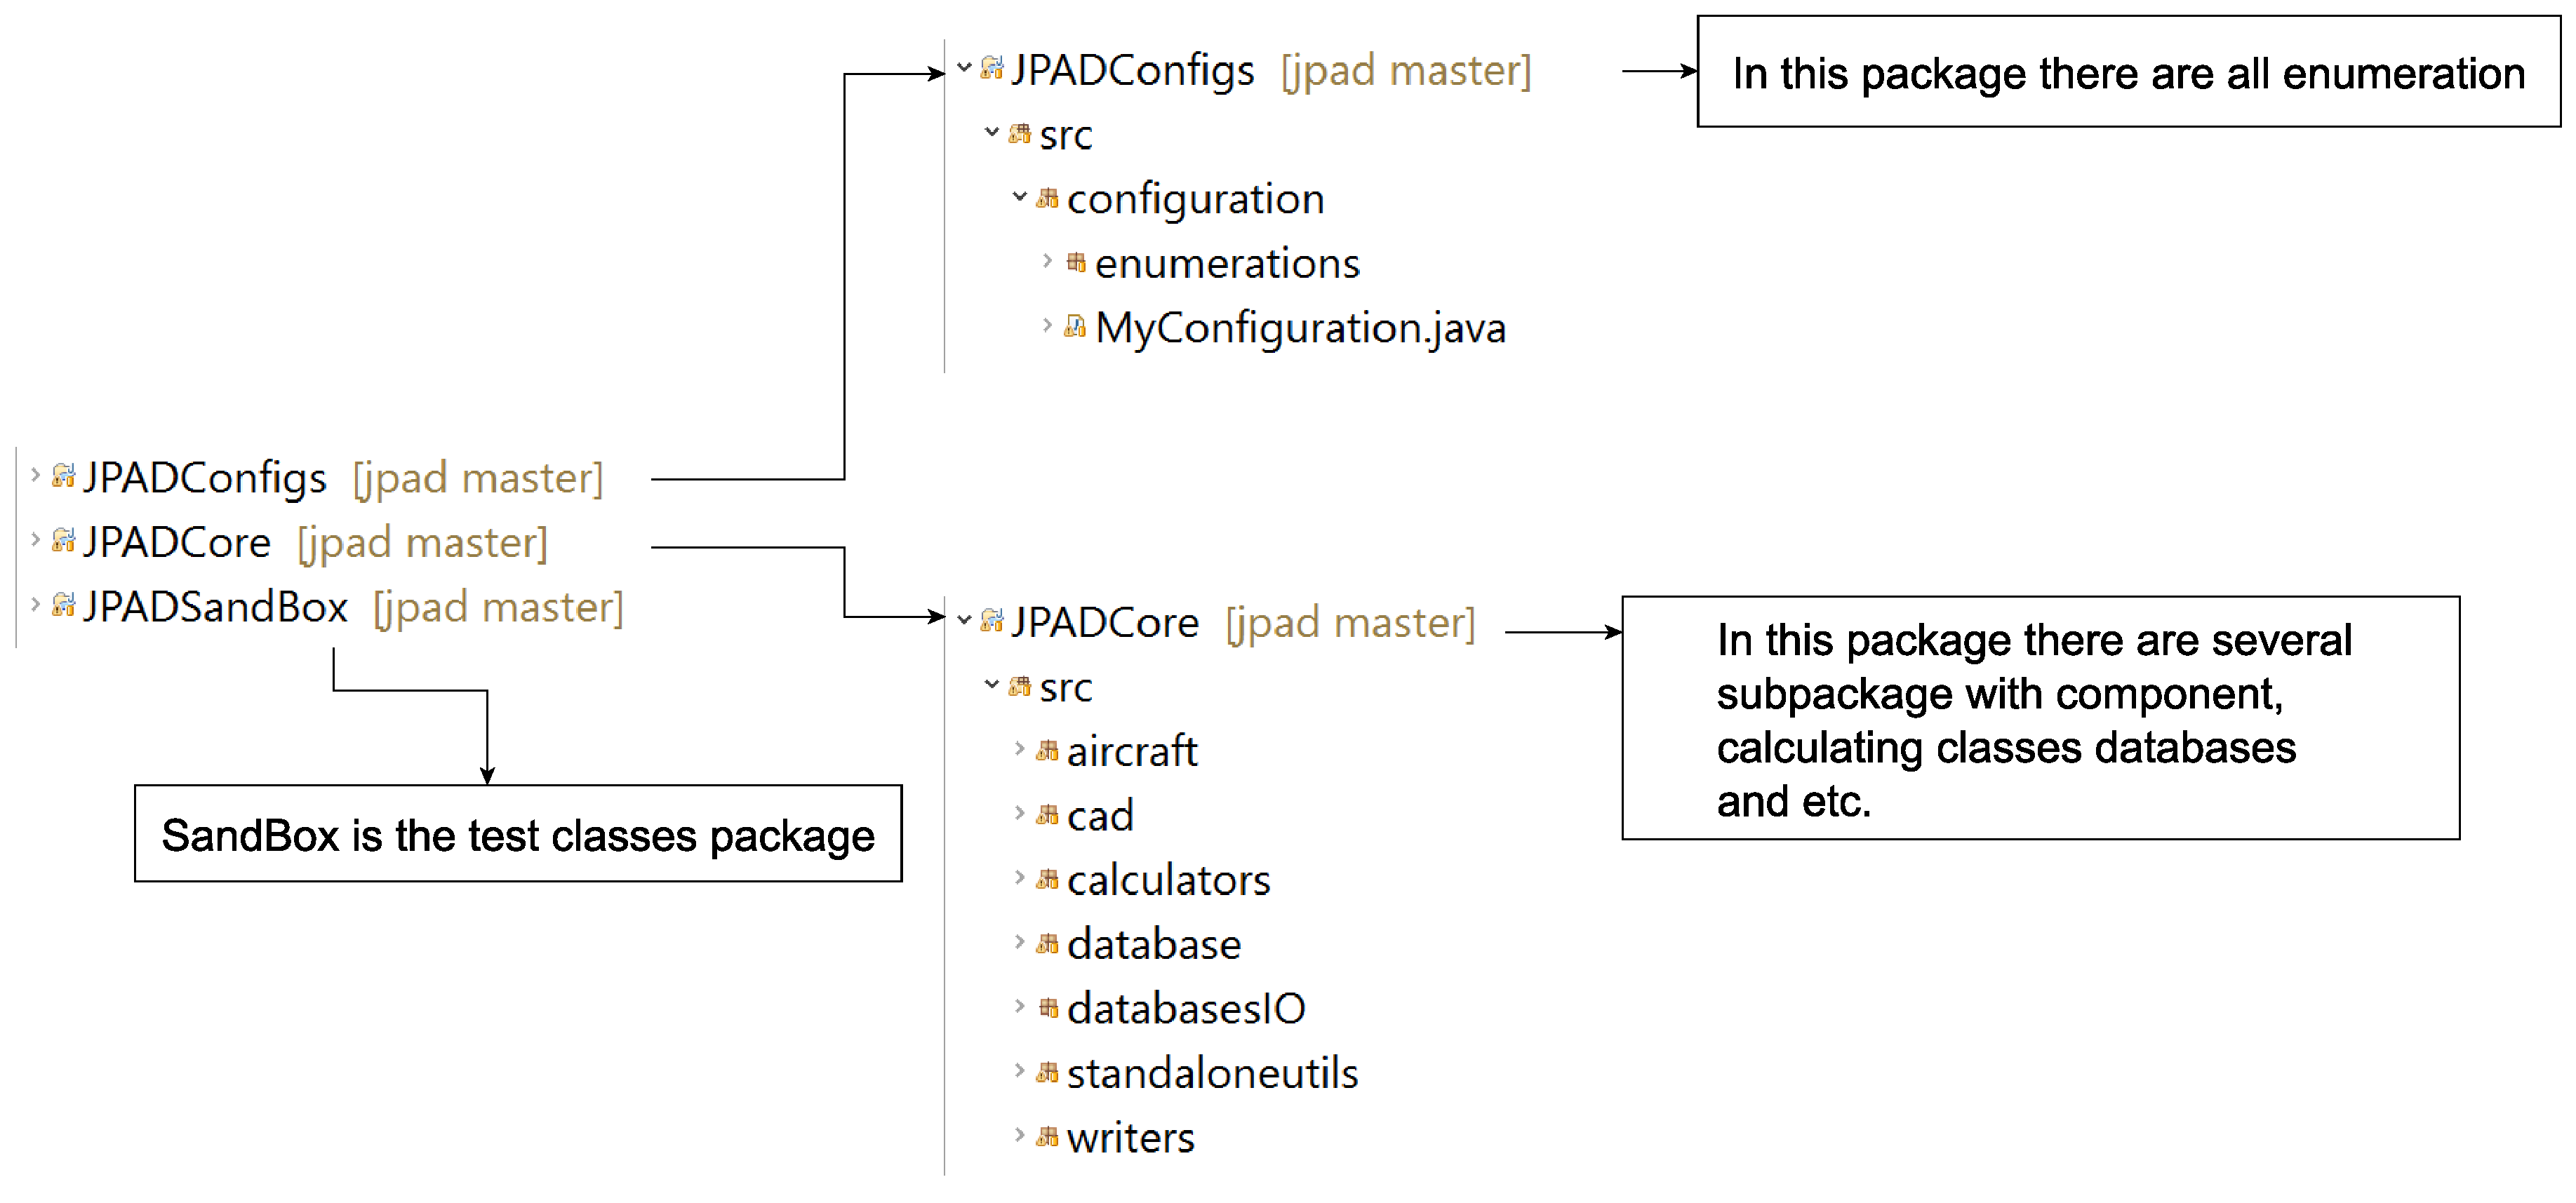
\includegraphics[height = 7.6cm ]{Immagini/organization}
	\caption{Software package division.}
	\label{fig:sw}
\end{figure}
 
 The main package of \gls{acr:Jpad} library is JPADCore where there are all aircraft component, the managers of calculator and  its computers classes. In the following subsection will explained the main features of JPADCore.\\
 JPADCore contains the following sub-packages:
 \begin{enumerate}
 \item \texttt{aircraft} $\rightarrow$ This package contains all aircraft's component classes, their calculators and the related managers and also the operating condition's class.
 \item \texttt{cad} $\rightarrow$  This package contains everything concerning the creation of CAD model.
 \item \texttt{calculators} $\rightarrow$ In this package there are the classes, divided in package by type of analysis, whose methods implement the calculation formulas.
 \item \texttt{database} $\rightarrow$ This package contains the classes that manage the database .h5 whose data are useful for the analysis. 
 \item \texttt{standaloneutils} $\rightarrow$ In this package there are several calculation classes with mathematical tools to support the analysis.
 \item \texttt{writers} $\rightarrow$ this class is in charge of writing files.
 \end{enumerate}
 
 \noindent \\
 Following will be explained the main features of the fundamental packages.
 
 \subsection{\texttt{Aircraft }package}
 Each component (e.g., the fuselage, the wing, the engine) is therefore defined in its own class. In the aircraft package there are other sub-package for components. In each of these there are a class for the object definition and a manager for the analysis. These manager classes uses the utilities located in the calculator package. \\
 The sub-package in the \texttt{aircraft} package are the following:
 
 \begin{itemize}
 \item \texttt{Auxiliary} that manages the airfoils
 \item  \texttt{Component} that contains the \texttt{aircraft} class, the aircraft components packages (fuselage, lifting surfaces, nacelles, power plant, fuel tank, landing gear, systems) and, inside them, their manager analysis classes used to call related analysis methods. 
 \item \texttt{OperatingConditions} 
 \end{itemize}

The main aircraft components are organised as follows: \\ 

Basic data for describing the {\bfseries fuselage} are contained in the \texttt{fuselage} class. This holds all the fuselage overall properties, such as the length, maximum width and maximum height, length ratios between the nose and the tail parts length to the constant section part length, number of decks and so on. Other classes in the package manage the shape of fuselage sections and outlines (which define the fuselage shape in the xz and xy planes) and aerodynamics calculations (Aerodynamics class).\\ \\

The data relating to the {\bfseries lifting surfaces} are contained in the \texttt{liftingSurface } class. Since the lifting surfaces of an aircraft share several characteristics, a single class has beencreated to manage the wing, the horizontal and vertical tail and, eventually, the canard. The lifting surface specific category (that is, wing, horizontal tail etc.) is acknowledged through a \texttt{MyComponentEnum} variable which has to be specified when creating the lifting surface object. By default, a lifting surface has three primary span stations: root ($\eta = 0$), middle and tip ($\eta = 1$). The middle station location is user-defined and is used to represent a change in chord.y/ law; such a change can be due to a lifting surface kink or to the beginning of a tapered part. If the wing is simple tapered the middle station can also be omitted.\\ \\

The data relating to the {\bfseries airfoils} are handled by \texttt{Airfoil} class, that creates for each lifting surface three airfoils, located respectively at $\eta=0$, $\eta=1$ and at middle station. An airfoil object holds:
\begin{enumerate}
	\item the position along the semispan, $\eta$;
	\item twist value relative to root, $\epsilon_g$;
	\item zero lift angle of attack, $\alphazlp$;
	\item angle of attack value at the end of the linear part of $C_l(\alpha)$ curve, $\alphastar$;
	\item stall angle of attack, $\alpha_{stall}$;
	\item lift gradient of the linear part of $C_l(\alpha)$ curve, $\Clalphap$;
	\item minimum drag coefficient, $C_{d,min}$;
	\item lift coefficient at $C_{d,min}$, $C_l@C_{d,min}$;
	\item lift cofficient at the end of linear part;
	\item maximum lift coefficient, $\Clmaxp$
	\item drag polar $K$ factor;
	\item aerodynamic moment coefficient gradient, $C_{m_\alpha}$;
	\item aerodynamic center x coordinate, $x_{ac}$;
	\item aerodynamic moment coefficient with respect to the aerodynamic center, $C_{m_{ac}}$ or $\Cmzerop$;
	\item aerodynamic moment coefficient with respect to the aerodynamic center at stall, $C_{m_{ac},stall}$;
	\item maximum thickness to chord ratio, $t/c_{max}$;
	\item x,z non dimensional coordinates.
\end{enumerate}
At the time of writing all these quantities have to be entered by the user. The \texttt{Airfoil} class provides the \texttt{populateCoordinateList()} method which transforms the non dimensional coordinates provided by the user in order to obtain their actual coordinates, which takes into account of actual chord length, ACRF position, sweep, twist and dihedral.\\ \\

The  {\bfseries power plant} is defined in the package \texttt{PowerPlant} in \texttt{components}. In this package there is the \texttt{engine} class that initializes the data related to the single engine. An other class in the same package, \texttt{powerPlant} creates the parametric model of the power plant using a list of objects creates by \texttt{engine}.


\subsection{\texttt{MyOperatingConditions} class}
As the name suggests, this class contains all the data related to atmosphere conditions (which are currently derived from altitude value using the 1976 ISA model), current speed (Mach number), gravitational acceleration (\SI{9.80665 }{\meter/\second^2}) and sea level pressure (\SI{101325}{\Pa}).

A \texttt{MyOperatingConditions} object can be created regardless of the aircraft configuration as the class is entirely self contained: the aircraft could also be undefined at the time of the object creation. If the user wants to run several analysis at different operating conditions, a \texttt{MyOperatingConditions} instance has to be created for each one.

\subsection{\texttt{CAD} package}

Throughout the development of the application, great care has been given to the making of the CAD model for several reasons:
\begin{itemize}
	\item it enables the user and the user developer to have an immediate feedback about the data provided to the application: if some geometrical parameter is wrong, the CAD model makes it impossible not noticing it;
	\item it allows the user to run a CFD analysis with an external program. The CAD model has been in fact built so that it is ready to be meshed by an external mesher without any further adjustment;
	\item it provides an accurate estimate of the wetted surface of each component.
\end{itemize}

The creation of the CAD model was made possible by the occjava library, whose classes and methods have been used to build each component's model.

 \subsection{\texttt{Calculators} package}
 This package includes all the calculators classes. Calculator classes have been created to evaluate quantities related with more than one component. The calculator classes are the following:
 
 \begin{itemize}
 \item {\texttt{aerodynamics} package}
\item {\texttt{cost} package}
\item {\texttt{geometry} package}
\item {\texttt{performance} package}
\item {\texttt{stability} package}
\end{itemize} 

Each of these package contains calculators classes and concerning methods that implement all mathematical equations. These methods are called by the analysis manager classes that are in the package of relatives components (such as fuselage, lifting surfaces etc.).

\subsection{\texttt{Database} package}
In order to manage a large quantity of data, it has been necessary to read data from graphs available in literature; for such a reason an extensive database has been built over the years by several of my colleagues to digitalize this data in order to exploit it in a computer program. The data has been stored in an hdf5 file.\\
In the \texttt{database} package there are all the classes that manage and reads the .h5 files. To obtain the useful data in JPAD, interpolating functions are used . These functions can be of one, two or three dimensions and read data from graphics that have been digitize previously.

\subsection{\texttt{Writers} package}
 This class is based on the Apache POI library and provides methods which enable the user developer to easily add a sheet to an XLS file, to set the styles of the XLS file and to compare different XLS files.The last function permits to create an XLS file which contains a different aircraft data for each column; in such a way the comparison between two or more aircraft (or,
simply, between slightly different configurations of the same aircraft) is easier and effective.



\section{Graphical User Interface (GUI)}
An extensive work has been done to set up an effective Graphical User interface (GUI) to reduce the time the user has to spend to obtain relevant results. The result presented in this section is the early step of graphical interface, which is currently in development.\\ 

The Java programming language greatly helped to build the GUI: several open source libraries (SWT, JFace) allowed us to build a functional yet pleasant GUI which allows the user to easily change the aircraft’s parameters, to view a 3D model of the defined geometry, to launch a new analysis and view the corresponding results. The current GUI appearance is shown in fig. \ref{fig:guiStart}. It is composed of several items:
\begin{enumerate}
	\item a menu bar (on top), which holds all the available actions divided in sub-categories;
	\item a toolbar (below the menu bar), which holds the most important actions needed to interact with the application. The toolbar, as the menu bar, is always visible to the user;
	\item a project tree (on the left), a key component of the GUI since it provides access to all the components of the aircraft and the analysis results any time during the execution of the application. The project tree appears once an aircraft is created and can be eventually hidden;
	\item a 3D view, which shows the CAD model of the aircraft selected by the user. The CAD model can be updated each time the user wants to check the changes made to the aircraft geometry;
	\item a log message window, placed at the bottom, that tells the user the status of pending operations. This window can be hidden;
	\item a tab folder, which contains all the windows opened using the project tree; these windows can be closed and reopened any time.
\end{enumerate}


\begin{figure}[H]
	\centering
	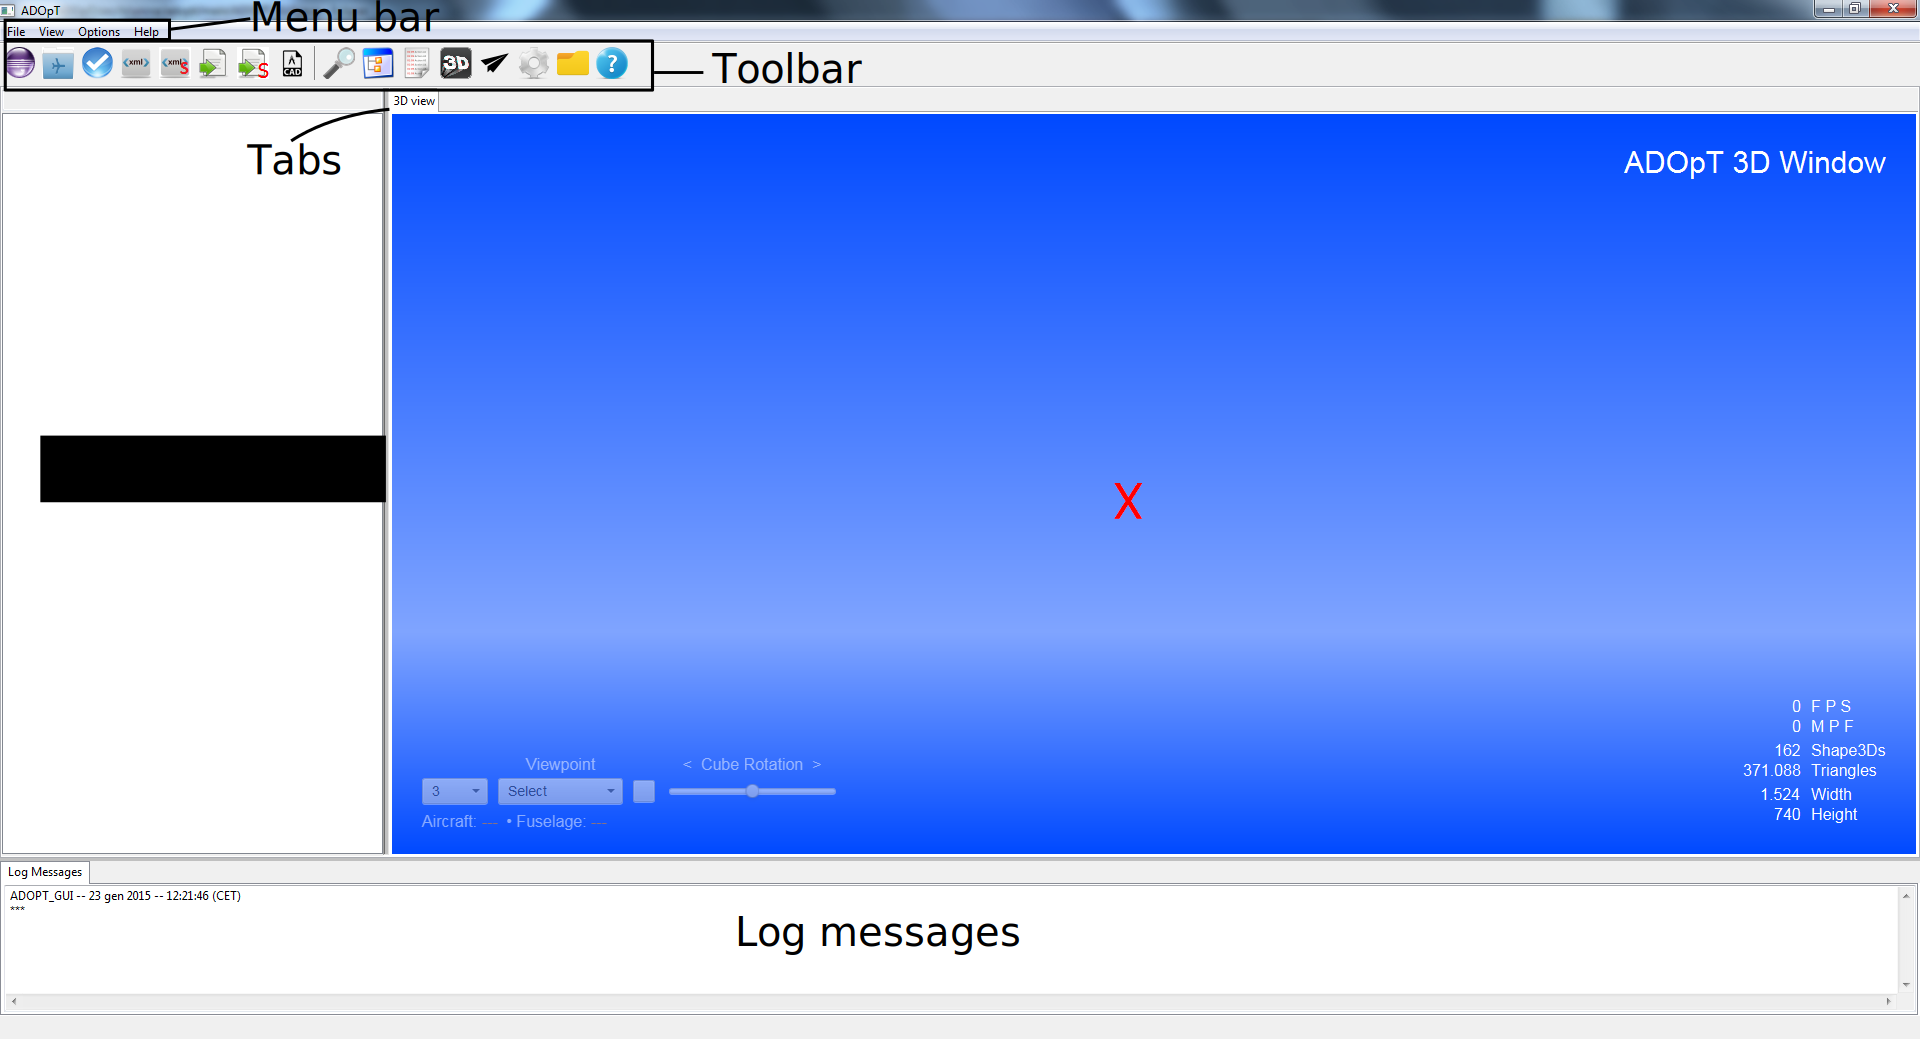
\includegraphics[height = 7cm ]{Immagini/gui/applicationStart.png}
	\caption{The GUI when the application is started.}
	\label{fig:guiStart}
\end{figure}

\subsection{Typical work session}
In developing the application we focused on making the user's typical work session as simple as possible. Few basics steps are required for running an analysis:

\begin{enumerate}
\item create a new aircraft, which we will call A. This can be done using the corresponding button \big(\includegraphics[scale=0.6]{Immagini/gui/icons/FolderAirplane_32x32.png}\big) in the toolbar, which instantiates the default aircraft
	
\item set the parameters that define the aircraft model using the corresponding window opened using the tree
\begin{figure}[H]
		\centering
		\includegraphics[height = 7cm]{Immagini/gui/changeFusParam.png}
		\caption{The window for changing the fuselage parameters.}
	\end{figure}
\item explore the 3D model \big(\includegraphics[scale=1.2]{Immagini/gui/icons/3DView_32x32.png}\big) of the aircraft and eventually change some parameters if there is some error
		\begin{figure}[H]
	\centering
		\includegraphics[height =7cm]{Immagini/gui/cad1.png}
		\caption{The aircraft 3D view (log window and project tree hidden).}
	\end{figure}
\item execute a complete analysis \big(\includegraphics[scale=0.5]{Immagini/gui/icons/analysis_32x32.png}\big) of the aircraft previously defined;

	\item export the analysis results to an XML and/or an XLS file \big(\includegraphics[scale=0.4]{Immagini/gui/icons/Export_32x32.png}\big);
	
	\item eventually export the CAD model of the aircraft \big(\includegraphics[scale=1.2]{Immagini/gui/icons/cad_32x32.png}\big);
	\item save the current aircraft to an XML file \big(\includegraphics[scale=0.4]{Immagini/gui/icons/XML_32x32.png}\big).
\end{enumerate}

	
At this point the user could simply change the current configuration until the analysis results are satisfactory. The application can however help the user in finding such a configuration, since it can hold multiple configurations simultaneously, analyse all of them and compare them side by side. To accomplish this task, once the first aircraft has been created, the user should:

\begin{enumerate}
	\item import the aicraft previously saved or create an entirely new aircraft, which we will call B;
	\item change B parameters and run a new analysis on it;
	\item study the results and eventually change some of the parameters;
	\item save every configuration and the corresponding results to file;
	\item export both aircraft and the corresponding results to an XLS file.
\end{enumerate}
	
	\begin{figure}[H]
	\centering
		\includegraphics[height =8cm]{Immagini/gui/cad3.png}
		\caption{The aircraft 3D view.}
	\end{figure}		
%

%\begin{figure}[H]
%		\centering
%		\includegraphics[height = 8cm ]{Immagini/gui/createAircraftDone.png}
%		\caption{The GUI as it appears when an aircraft is created.}
%		\label{fig:guiDescription}
%	\end{figure}


There is no limit to the number of aircraft the application can handle; each aircraft is added to the project tree as shown in fig. \ref{fig:projectTreeMulti} providing access to the corresponding components and analysis.

\begin{figure}[H]
	\centering
	\includegraphics[height=8cm]{Immagini/gui/projectTreeMulti.png}
	\caption{The project tree holding two different aircraft}
	\label{fig:projectTreeMulti}
\end{figure}

\begin{figure}[h]
	\centering
	\includegraphics[width=5cm]{Immagini/gui/tabId.png}
	\caption{Same component tab belonging to different aircraft}
	\label{fig:tabId}
\end{figure}



\subsection{CAD modelling}
The application can also be used as a basic parametric \gls{acr:cad} modeler. The capability to change the aircraft parameters using the corresponding controls in the \gls{acr:gui}, coupled with the 3D view, allows the user to change each component shape and dimension, view the updated \gls{acr:cad}model and eventually export it to file once some satisfactory results have been obtained.\\
The creation of the CAD model was made possible by the occjava library, whose classes and methods have been used to build each component’s model. The CAD model can be saved in two different file formats: STEP and BREP; they have proven to take both little memory and to give the best results in terms of geometry representation. The IGES format gave instead mixed results so we preferred to use only the first two.

\begin{figure}[H]
	\centering
		\includegraphics[width=6 cm]{Immagini/gui/CADfuselageTailBAD2.png}
		\caption{A detail of the tail of the fuselage obtained as a unique loft.}
		\label{fig:badTail}
	\end{figure}
	
	\begin{figure}[H]
	\centering
		\includegraphics[width=6 cm]{Immagini/gui/CADfuselageTailOK.png}
		\caption{A detail of the tail of the fuselage obtained sewing together its parts.}
		\label{fig:goodTail}
\end{figure}


	\begin{figure}[H]
	\centering
		\includegraphics[width=12 cm]{Immagini/gui/CADfuselage}
		\caption{External fuselage shape exported as STEP file.}
		\label{fig:goodTail}
\end{figure}


\subsection{Interface with external software}
With ADOpT it's also possible to execute some high-fidelity analyses using external tools (i.e. CFD Navier-Stokes solver, panel method, FEM for structural static and dynamic analysis, etc.) by importing the dedicated output (such as a CAD model) produced by the software. The higher-fidelity tools could improve the results obtained and give therefore some useful clues in order to start a new design loop with different requirements and/or different constraints. The possibility to interface the software with drawings and graphical representation (i.e. CAD or Catia) of the designed aircraft is also very important.

\begin{figure}[H]
	\centering
		\includegraphics[width=12 cm]{Immagini/interface}
		\caption{Interface with external CFD tools.}
		\label{fig:badTail}
	\end{figure}
	
\section{In Development}


\part{Development of Application}
\chapter{Introdution to Java}
\label{ch:java}
\markboth{Introdution to Java}{}


\begin{flushright}
	{\smaller
		\textit{Language is only the instrument of science, \\and words are but the signs of ideas.}\\
		-- Samuel Johnson}
\end{flushright}


\section{The java Language}
The term Java refers both to a programming language with the higher number of developers in the worldwide and to a technology that has several sub-technologies that have emerged in different fields of use of the software. Javawas developed by Sun Microsystems, a company that was incorporated in Oracle from a few years.
In 1996, James Gosling, Bill Joy, and Guy Steele wrote for the First Edition of The Java Language Specification:
``{\itshape We believe that the Java programming language is a mature language, ready for widespread use. Nevertheless, we expect some evolution of the language in the years to come. We intend to manage this evolution in a way that is completely compatible with existing applications.}''\\
This programming language is a general-purpose, concurrent, classbased, object-oriented language. It is designed to be simple enough that many programmers can achieve fluency in the language.\cite{javaoracle}
One design goal of Java is portability, which means that programs written for the Java platform must run similarly on any combination of hardware and operating system with adequate runtime support. This is achieved by compiling the Java language code to an intermediate representation called Java bytecode, instead of directly to architecture-specific machine code. Java bytecode instructions are analogous to machine code, but they are intended to be executed by a virtual machine (VM) written specifically for the host hardware. End users commonly use a Java Runtime Environment (JRE) installed on their own machine for standalone Java applications, or in a web browser for Java applets.\cite{wiki:java}
Standard libraries provide a generic way to access host-specific features such as graphics, threading, and networking.\\
There were five primary goals in the creation of the Java language:\cite{java}
\begin{enumerate}
\item It must be ``simple, object-oriented, and familiar''.
\item It must be ``robust and secure''.
\item It must be ``architecture-neutral and portable''.
\item It must execute with ``high performance''.
\item It must be ``interpreted, threaded, and dynamic''.
\end{enumerate}
Java SE 8 represents the single largest evolution of the Java language in its history. A relatively small number of features - lambda expressions, method references, and functional interfaces - combine to offer a programming model that fuses the objectoriented
and functional styles. Under the leadership of Brian Goetz, this fusion has been accomplished in a way that encourages best practices - immutability, statelessness, compositionality - while preserving ``the feel of Java'' - readability, simplicity, universality.\\
Actually Java is the most used programming language according to TIOBE. The TIOBE Programming Community index is an indicator of the popularity of programming languages. The ratings are based on the number of skilled engineers world-wide, courses and third party vendors.


\section{Java choice}

The software presented in this thesis work is completely written in Java. The choice of the programming language was driven by several considerations. These include the following:

\begin{itemize}
\item the language should be widely supported; this to avoid the case of many valid aircraft design applications and libraries that became obsolete due to the aging of the programming language used to build them;
\item the language should promote the use of open source libraries, especially for I/O tasks and for complex mathematical operations;
\item the language and the companion \gls{acr:ide} should provide a widely supported \gls{GUI} framework and a \gls{GUI} visual builder;
\item  the language should support and promote modularity.
\end{itemize}
The Java programming language meets all these requirements: it is backed by Oracle and by a huge community of developers so it is continuously updated. Also, advanced and free \gls{acr:ide}s (such as Eclipse) allow programmers to streamline and simplify the development process. In particular, the Eclipse \gls{acr:ide} and the SWT/JFace libraries have been chosen to develop \gls{acr:Jpad} and its \gls{GUI}.
Being Java a pure object oriented programming language, it greatly encourages and simplifies modularization. Each module (package) can be programmed quite independently so that it is relatively easy to divide the work among several programmers. This is essential since the amount of classes and calculations needed to abstract, manage and analyze the entire aircraft is very large (presently the whole project counts more than 56000 lines of code). For such a reason the establishment of common practices and the adherence to fundamental principle of software development (Don’t Repeat Yourself, Separation of Concerns, Agile software development) are equally important.
An important design requirement of \gls{acr:Adopt} is related to its interoperability with other engineering analysis tools. In fact, the application can be easily integrated into a comprehensive aircraft optimization cycle. This is made possible because \gls{acr:Adopt} can be launched both in \gls{GUI} and command line mode. Much care has been given to input/output and configuration files to increase the possible uses of the software.\cite{adoptunina}

\begin{figure}[H]
\centering
{\includegraphics[height=7.6cm ]{Immagini/trend.png}} 
\caption{Programming Language popularity trade.}
\label{fig:hl}
\end{figure}







\chapter{Work Object}%
\label{ch:workobject}
\markboth{Work Object}{}

\begin{flushright}
	{\smaller
		\textit{Citazione}\\
		-- Autore}
\end{flushright}

\section {Introduction}
In JPAD it is possible to read an .XML file as input or generate an object whose data are written in the code. Both in the first and in the second case all needed variables are initialized with data relating the choosen aircraft. The difference between these two methos is that using an .XML file, user can to define its own aircraft having clear view about the needed data useful for the analysis.\\
Contrariwise in order to perform test of program functionality, to use a default aircraft is the most simple way to generate a work object.

\section {Input data from .XML file}
\subsection{XML File Format}
XML is a file extension for an {\itshape Extensible Markup Language (XML)} file format used to create common information formats and share both the format and the data on the World Wide Web, intranets, and elsewhere using standard ASCII text.
It is defined ``Markup Language'' due to the use of tags that describes the content. XML is considered extensible because the markup symbols are unlimited and self-defining. So it is possible to use parsonal tag for each data. \\
In this way it results relatively simple to read an .XML file.\\
The key concepts of an .XML File Format are the followings:
\begin{itemize}
\item markup symbol (tag)
\item attribute
\item tree structure
\end{itemize}

As mentioned each part of the test is contained between an opening {\bfseres markup symbol} and an end markup symbol that expressed the meaning of the test.\\

\begin{figure}[H]
\centering
{\includegraphics[height=0.39cm]{Immagini/xml1.jpg}} 
\caption{Use of markup symbol in XML language.}
\end{figure}

In addition to tag name, the markup symbols may contain also some {\bfseries attributes} that introduce more informations such as the unit of measure.\\

\begin{figure}[H]
\centering
{\includegraphics[height=0.4cm]{Immagini/xml2.jpg}} 
\end{figure}

An .XML file ha a tree structure where there extenal knots that branch in internal knots.
%TODO add second image


\begin{figure}[H]
\centering
{\includegraphics[height=6cm]{Immagini/xml5.jpg}} 
\caption{Tree structure of an .XML file.}
\end{figure}

\subsection{Reading data from an .XML file.}
%JPADDATAWRITER 
%possibili sviluppi futuri

\section {Default Aircraft}
\subsection {How is made a default Aircraft in JPAD}
%foto grafico 

\subsection {How is made a default Wing in JPAD}
% scrivi che è possibile costruire solo l ala come ho fatto io

\section {Database in JPAD}

In JPAD it is possible to consult external databases in .h5 format. {\bfseries HDF 5} (Hierarchical Data Format Release 5) is a data file format designed by the {\itshape National Center for Supercomputing Applications} (NCSA) to assist users in the storage and manipulation of scientific data across different operating systems and machines.\\
To obtain the useful data in JPAD  interpolating functions are used . These functions can be of one, two or three dimensions and read data from graphics that have been digitize previously.\\
Starting from these digitalizations, databases in .h5 format are built.
Reading data from databases is entrusted to methods of classes in the \texttt{database} package.\\
In order to read these databases, and obtain the useful data, it is necessary to define an object of the database reading class and associate it with the object of analysis.\\
This is a crucial step to read correctly the external data. In fact JPAD allows to work with an aircraft object  or only with an isolated lifting surface object.  Aircraft is usually composed of a fuselage, lifting surfaces, nacelle and power plant.
Furthermore, \texttt{Aircraft} and \texttt{Wing} are associated with classes of calculation like \texttt{LSAerodynamicManager} or \texttt{ACAnalysisManager}. So it is necessary that these databases are also visible from these classes.\\
So because  both in aircraft and in wing there is a lifting surface object, databases relative to wing are associated to \texttt{LSAerodynamicManager}.


\subsection {Initialize working directory tree}

First of all it is necessary to initialize the working directory tree. This step is required in order to create the following default folders that are necessary for the right behavior of the code:

\begin{itemize}
\item Database directory
\item Input directory
\item Output directory
\end{itemize}


To set the working directory with the useful folders, it's necessary to call the function \texttt{initWorkingDirectoryTree()} at the beginning of each test. The function creates all necessary folders. Morover the function has been overloaded and it can be even called with a variable number of arguments (\texttt{initWorkingDirectoryTree( String...str)}). These strings are the directory strings in \texttt{MyConfiguration} class.


\subsection {Setup database}
Here the database path it's created and associated to object that interpolates the required data from the .h5 file using a \texttt{MyInterpolatingFunction} object. After this it's possible to access the double value of the interpolating function using the \texttt{standaloneutils} method called \texttt{value}. \\


%\begin{lstlisting}[frame=rbl,caption={{\footnotesize Setup database(s)}},label= [style=\bfseries]{Listing}]
%// --------------------------------------------------------------
%// Define database
%// --------------------------------------------------------------
%MyConfiguration.initWorkingDirectoryTree();
%
%// Setup database(s)	
%String databaseFolderPath = MyConfiguration.getDir(FoldersEnum.DATABASE_DIR);
%String databaseFileName = "Aerodynamic_Database_Ultimate.h5";
%AerodynamicDatabaseReader aeroDatabaseReader = 
%		new AerodynamicDatabaseReader(
%				databaseFolderPath, 
%				databaseFileName
%				);
%\end{lstlisting}

Now the procedure to assign the database is different if is used an Aircraft object or a Wing object.

\subsection {Assign database using an Aircraft object}
In order to assign correctly the database and associate it to all analysis management is necessary to practise the following order.
\begin{enumerate}
\item Define an Aircraft Object.\\This command associates to Aircraft an object that defines the aerodynamic. From the wing it is possible to obtain the Wing, that is a \texttt{LiftingSurface} object.
\item Define an \texttt{ACAnalysisManager} object.\\All the aircraft computations are managed by this class.
\item Define an \texttt{LSAerodynamicManager} object.\\ All the lifting surfaces computations are managed by this class.
\item Associate database to \texttt{LSAerodynamicManager}.
\item Eventually do analysis.
\end{enumerate}

\subsection {Assign database using a Wing object}
Using a Wing object it isn't neccessary to define a manager for Aircraft aerodynamic analysis. So the step to follow are the same of aircraft starting from the third.
\begin{enumerate}
\item Define an Wing Object.
\item Define an \texttt{LSAerodynamicManager} object.
\item Associate database to \texttt{LSAerodynamicManager}.
\end{enumerate}

The definition of a isolated Wing is explained in the relative chapter.

%\begin{lstlisting}[frame=rbl,caption={{\footnotesize Assign database using an Aircraft object}},label= [style=\bfseries]{Listing}]
%
%// --------------------------------------------------------------
%// Generate default Aircraft
%// --------------------------------------------------------------
%Aircraft aircraft = Aircraft.createDefaultAircraft("B747-100B");
%LiftingSurface theWing = aircraft.get_wing();
%		
%// Default operating conditions
%OperatingConditions theConditions = new OperatingConditions();		
%		
%		
%// --------------------------------------------------------------
%// Define an ACAnalysisManager Object
%// --------------------------------------------------------------
%ACAnalysisManager theAnalysis = new ACAnalysisManager(theConditions);
%theAnalysis.updateGeometry(aircraft);
%		
%		
%// --------------------------------------------------------------
%// Define an LSAerodynamicsManager Object
%// --------------------------------------------------------------
%LSAerodynamicsManager theLSAnalysis = new LSAerodynamicsManager ( 
%		theConditions,
%		theWing,
%		aircraft
%		);
%		
%		
%// --------------------------------------------------------------
%// Associate database to LSAerodynamicManager
%// --------------------------------------------------------------
%theLSAnalysis.set_AerodynamicDatabaseReader(aeroDatabaseReader);
%
%		
%// --------------------------------------------------------------
%// Do analysis
%// --------------------------------------------------------------
%theAnalysis.doAnalysis(aircraft, 
%		AnalysisTypeEnum.AERODYNAMIC);
%\end{lstlisting}

\noindent \\
\begin{lstlisting}[frame=rbl,caption={{\footnotesize Assign database using an Aircraft object}},label= [style=\bfseries]{Listing}]
public static void main(String[] args) {

	// --------------------------------------------------------------
	// Define directory
	// --------------------------------------------------------------
	MyConfiguration.initWorkingDirectoryTree();


	// --------------------------------------------------------------
	// Generate default Aircraft
	// --------------------------------------------------------------
	Aircraft aircraft = Aircraft.createDefaultAircraft("B747-100B");
	LiftingSurface theWing = aircraft.get_wing();

	// Default operating conditions
	OperatingConditions theConditions = new OperatingConditions();		


	// --------------------------------------------------------------
	// Define an ACAnalysisManager Object
	// --------------------------------------------------------------
	ACAnalysisManager theAnalysis = new ACAnalysisManager(theConditions);
	theAnalysis.updateGeometry(aircraft);


	// --------------------------------------------------------------
	// Define an LSAerodynamicsManager Object
	// --------------------------------------------------------------
	LSAerodynamicsManager theLSAnalysis = new LSAerodynamicsManager ( 
			theConditions,
			theWing,
			aircraft
			);

		
	// --------------------------------------------------------------
	// Setup database(s)	
	// --------------------------------------------------------------
		
	theLSAnalysis.setDatabaseReaders(
			new Pair(DatabaseReaderEnum.AERODYNAMIC,
                          "Aerodynamic_Database_Ultimate.h5"),
			new Pair(DatabaseReaderEnum.HIGHLIFT,  
                          "HighLiftDatabase.h5")
			);

	
	// --------------------------------------------------------------
	// Do analysis
	// --------------------------------------------------------------
	theAnalysis.doAnalysis(aircraft, 
			AnalysisTypeEnum.AERODYNAMIC);
}
\end{lstlisting}
The databases are assigned to \texttt{LSAerodynamic} using a method of this class. This method accept as input a variable number of \texttt{Pair} objects.Using \texttt{Pair} objects it is possible to assign, for each database, both name and type. 

\noindent \\
\begin{lstlisting}[frame=rbl,caption={{\footnotesize \texttt{setDatabaseReaders} method}},label= [style=\bfseries]{Listing}]

public void setDatabaseReaders(Pair... args) {
	String databaseFolderPath = MyConfiguration.getDir(FoldersEnum.DATABASE_DIR);
	
	for (Pair a : args) {
		DatabaseReaderEnum key = (DatabaseReaderEnum)a.getKey(); 
		String databaseFileName = (String)a.getValue();
		
		switch (key) {
			case AERODYNAMIC:
				_aerodynamicDatabaseReader = 
				new AerodynamicDatabaseReader(
						databaseFolderPath,
						databaseFileName); 
				listDatabaseReaders.add(_aerodynamicDatabaseReader);
				break;
				
			case HIGHLIFT:
				_highLiftDatabaseReader = 
				new HighLiftDatabaseReader(
						databaseFolderPath, 
						databaseFileName); 
				listDatabaseReaders.add(_highLiftDatabaseReader);
			break;	
			
		}
\end{lstlisting}


\subsection {Developer's guide}

In order to execute some analysis in JPAD it is necessary, first of all, to define an analysis object in the Test class. The method \texttt{createDefaultAircraft} creates a new aircraft and the object that composes it. This method also populates the data of aircraft with default value corresponding to ATR-72 or Boieng 747\_100B. Moreover the method \texttt{createDefaultAircraft} calls another method in \texttt{Aircraft} class: \texttt{initialize} that initializes the objects of the classes that perform calculations. \\
The purpose of this structure is to have only a way to assign the databases at an aircraft. Inasmuch as the wing is always present, the chosen strategy is to assign the database to the aerodynamic manager of the wing.\\
In order to bring to use the database also for the aircraft calculation, it is assigned at the aerodynamic manager of the aircraft in the method called \texttt{doAnalysis}.\\
At the same time \texttt{LSAerodynamicManager} sets itself as aerodynamic in the wing object. \\
So it is possible to call the database using equally the following codes: 
\begin{itemize}
\item \texttt{theWingObject.getAerodynamics.get\_Database;}
\item \texttt{theAircraftObject.get\_theAerodynamic.get\_Database;}
\item \texttt{theLSManagerObject.get\_Database;}
\item \texttt{theACManagerObject.get\_Database;}
\end{itemize}

\begin{sidewaysfigure}

\centering
\includegraphics[width=23cm]{immagini/HowToAssignDatabase.jpg}
\caption{Flow chart of database assignment.}
\label{fig:schemauno}

\end{sidewaysfigure}

\part{Functionality Overview}
\chapter{Wing Lift Characteristics}
\label{ch:worklift}
\markboth{Wing Lift Characteristics}{}

\begin{flushright}
	{\smaller
		\textit{C'è qualcuno che può rompere il muro del suono,\\ mentre tutto il mondo si commenta da solo.}\\
		-- L. Ligabue}
\end{flushright}


Any body in motion in a fluid presents a result of force acting on it, which can be decomposed in two components:
\begin{itemize}
\item A {\bfseries Lift} acting normal to the Velocity direction and is positive upward.
\item A {\bfseries Drag} acting in the opposite direction to the airspeed vector.
\end{itemize}
The lifting surfaces of an airplane are designed to generate lift exceeding their drag, in order to obtain a positive efficiency. \\ In this chapter it will be explained how it is possible to evaluate the complete lift coefficient curve of a wing, both in its linear trait and non linear.\\
The lift coefficient is a dimensionless number used to model all of the complex dependencies of shape, inclination, and some flow conditions on lift. The lift coefficient also contains the effects of air viscosity and compressibility that are molded respectively with the Raynolds and Mach number.% [ Cap. \cite{nasaLift}] 

\section{Theoretical background}

In order to achieve the complete curve of coefficient list it is necessary to obtain the following parameters:

\begin{enumerate}
\item Zero-Lift Angle
\item Lift Coefficient slope 
\item End of Linearity Angle
\item Maximum Lift Coefficient
\item Stall Angle of attack
\end{enumerate}

Following it will be explained the theory behind how these contributions have been made.

\subsection{Zero-Lift Angle and Lift Coefficient Slope}

In order to evaluate the linear trait of the wing lift curve, it is been used the Nasa-Blackwell method.\\ The {\bfseries Nasa-Blackwell} is a numerical method for calculating the subsonic load distribution for arbitrary lifting surface arrangements at a fixed angle of attack. The method is suitable for swept wings, non-planar wings, wing with pylons and/or end-plates; it can be also used to study the aerodynamic interaction of the wing and the horizontal tail. The method has been implemented because its results, as shown in the report, were in good agreement with the experimental results.
The lifting surfaces are divided in several rectangular horse-shoe vortices along the span; one horseshoe vortex along the chord is used, that is, the midpoints of the vortices are placed only at points along the quarter-chord lines. An equal number of control points are located along the three-quarter-chord lines. The velocity from the total vortex system is equated to the component of free-stream velocity normal to the lifting surface chord at each control point. Application of this tangent-flow boundary condition for a symmetrical loading provides a set of N simultaneous equations in the N unknown circulation strengths. Solution of this set of equations provides the loading distributions over the lifting surfaces. Mach number effect is introduced through a Prandtl-Glauert correction. Further details can be found in \cite{NASA:Blackwell}.

In this way  the Zero Lift angle it is calculated using the integral of the load distribution and the linear trait slope starting from the value of CL at $\alpha =  0^{\circ}$ and $\alpha = 2^{\circ}$.

\begin{equation}
CL_{\alpha}= \frac{CL|_2 - CL|_0}{\upDelta \alpha}
\end{equation}

In JPAD it is possible also evaluating these two contributes using different methods. \\
For the evaluation of the $\alpha_{0L}$ it is possible to use a method of the class \texttt{CalcAlpha0L}, a nested class  in \texttt{LSAerodynamicManager}. Using these method, the zero-lift angle is calculated with the following formula, where $\epsilon_T$ is the twist angle:

\begin{equation}
\alpha_{0L} = \frac{1}{S}\int_{-\frac{b}{2}}^{\frac{b}{2}} c(y) [ \alpha_0(y) - \epsilon_T(y) ] \, dy
\end{equation}

This formula  is applied to the exposed wing. When a default aricraft is defined, during the creation of components, is calculated the exposed wing. This is the wing outside of the fuselage. It starts at semi-diameter of fuselage and its root airfoil is the airfoil of wing  at this station calculated by the method \texttt{calculateIntermediateAirfoil}.\\ \\

In order to evaluate the lift coefficient linear slope  it is possible to use different method belonging to \texttt{CalcCLAlpha} class. The first one use the Polhamus formula which is valid for arbitrary aspect ratios and sweep angles in subsonic flow:

\begin{equation}
CL_{\alpha} = \frac{2 \pi \AR}{ \left\{ 2 + \sqrt{\frac{\AR^2 \beta^2}{k^2} \left ( 1 + \frac{\tan^2{(\Lambda_{\frac{c}{2}})}}{\beta^2} \right) + 4 }\right\}}
\end{equation}

Thus $CL_{\alpha}$  is a function of wing aspect ratio, mid-chord sweep angle $\Lambda_{\frac{c}{2}}$, Mach number, and airfoil section (defined parallel to the free stream) lift curve slope. The factor K in the equation is the ratio of the experimental two-dimensional lift curve slope.\\
Alternately it is possible to use the Anderson formula for swept wing, compressible and subsonic flow:

\begin{equation}
CL_{\alpha} = 
\frac{Cl_{\alpha} \cos{\Lambda_{\frac{c}{2}}}}
{\sqrt{1 - M^2  cos^2 {\Lambda_{\frac{c}{2}}}
 + \left[ \frac{Cl_{\alpha} \cos{\Lambda_{\frac{c}{2}}}}{\pi \AR}\right]^2} + \frac{Cl_{\alpha} \cos{\Lambda_{\frac{c}{2}}}}{\pi \AR}}
\end{equation}



\subsection{End of Linearity angle of attack}

The angle of end linearity is calculated using the characteristics of the mean airfoil of the wing. This is obtained through the influence area of the airfoils as shown in fig. \ref{fig:influencearea}.

\begin{figure}[H]
\centering
{\includegraphics[height=3cm]{Immagini/influencearea}} 
\caption{Influence area of the sections for finite wing.}
\label{fig:influencearea}
\end{figure}

Then is possible to calculate the influence coefficients. 

\begin{equation}
K_i = \frac{2 S_i}{S}
\end{equation}

The mean parameters can be obtained from:

\begin{equation}
\overline{x} = x_1 K_1 + x_2 k_2 +x_3 k_3...
\end{equation}

In particular, for a wing defined by three airfoils, the end of linearity angle of attack is obtained from the following equation:

\begin{equation}
\alpha^* = \alpha^*_{1} K_1 + \alpha^*_{2} k_2 +\alpha^*_{3} k_3
\end{equation}

\subsection{Maximum Lift Coefficient}

In order to evauate the maximum lift coefficient the Stall Path Method has been used. The load distribution is calculated using Nasa-Blackwell method.

\begin{figure}[H]
\centering
{\includegraphics[height=6cm]{Immagini/Loading_Stall_Path_A}} 
\caption{Determination of wing lift distribution and Cl distribution of airfoils.}
\label{fig:stall0}
\end{figure}




The  practiced procedure is the following:

\begin{enumerate}
\item For each value of an Alpha array the load distribution is calculated using the NasaBlack method.  The distribution of  $Cl_{max}$ is known. fig. \ref{fig:stall1}.
\item At $\alpha = \alpha_j$ the load distribution curve intersects for the first time the $Cl_{max}$ curve of the airfoils. fig. \ref{fig:stall1}.
\item For each $ y > y_1 $ , along y axis (where y_1 is the station of first intersection) is evaluated the difference between $CL_{wing}$ and $Cl_{max}$. fig. \ref{fig:stall2}.
\item $\upDelta \alpha$ is evaluated until the maximum difference between $CL_{wing}$ and $Cl_{max}$ is smaller than the required accuracy. Actually the accuracy is 0.0001. 
\end{enumerate}

The evauation of $\upDelta \alpha$ is not simple.\\
After finding the first value of intersection between $CL_{wing}$ and $Cl_{max}$ a new $\alpha$ is evaluated. The first value used for the optimization is 

\begin{equation}\notag
\upDelta \alpha = \alpha_j -\alpha_{j-1}
\end{equation}
\begin{equation}\notag
\alpha_{new} = \alpha_j - \frac {\upDelta \alpha }{2}
\end{equation}
\begin{equation}\notag
\alpha_{old}= \alpha_j
\end{equation}

For the following step if there isn't a point of intersection at $\alpha_{new}$ the new value of $\alpha$ is, for the step $j+1$:


\begin{equation}\notag
\upDelta \alpha = |\alpha_{j-1} -\alpha_{j}|
\end{equation}
\begin{equation}\notag
\alpha_{new} = \alpha_{j} + \frac {\upDelta \alpha }{2}
\end{equation}
\begin{equation}\notag
\alpha_{old}= \alpha_j
\end{equation}

Instead,  if there is a point of intersection at $\alpha_{new}$ the new value of $\alpha$ is, for the step $j+1$:


\begin{equation}\notag
\upDelta \alpha =  |\alpha_{j-1} -\alpha_{j}|
\end{equation}
\begin{equation}\notag
\alpha_{new} = \alpha_{j} - \frac {\upDelta \alpha }{2}
\end{equation}
\begin{equation}\notag
\alpha_{old} = \alpha_j
\end{equation}



\begin{figure}[H]
\centering
{\includegraphics[height=6cm]{Immagini/Loading_Stall_Path_B}} 
\caption{Determination of wing lift distribution and Cl distribution of airfoils.}
\label{fig:stall1}
\end{figure}


\begin{figure}[H]
\centering
{\includegraphics[height=6cm]{Immagini/Loading_Stall_Path_D}} 
\caption{Intersection  between $CL_{wing}$ and $Cl_{max}$ curves.}
\label{fig:stall2}
\end{figure}

\begin{figure}[H]
\centering
{\includegraphics[height=6cm]{Immagini/Loading_Stall_Path_E}} 
\caption{Determination of $\upDelta \alpha$.}
\label{fig:stall5}
\end{figure}

\begin{figure}[H]
\centering
{\includegraphics[height=8.3cm]{Immagini/wing_loading_B}} 
\caption{Wing Loading distribution.}
\label{fig:wl}
\end{figure}

\subsection{Stall Angle of Attack}

Nasa-Blackwell is an inviscid method for calculating the subsonic aerodynamic load distributions for arbitrary lifting-surface arrangements. This means that it does not see the non linear trait of the lift curve. So in correspondence of the value of $C_{L_{MAX}}$ calculated, the angle of attack obtained from the Nasa-Blackwell method is not correct because it is the maximum angle of attack that you would get if you reach the max $C_L$ linearly.\\
So first it is evaluated the angle of attack at maximum lift coefficient through the linear trend of the lift line, then it’s added to this angle the increment evaluated by the diagram in fig. \ref{fig:dealpha}, this is valid strictly for wing with high taper ratio without twist, with unique airfoil type and Mach number included between 0.2 and 0.6.


\begin{figure}[H]
\centering
{\includegraphics[height=6.3cm]{Immagini/deltaAlphaSforza.png}} 
\caption{Diagram useful for evaluation of $\upDelta \alpha$.}
\label{fig:dealpha}
\end{figure}



\subsection{Construction of the curve}
At this point all elements are available in order to draft the CL vs $\alpha$ curve.\\ The linear trait is evaluated using the equation of straight line.

\begin{equation}
C_L= C_{L_\alpha} \alpha + C_{L_0}
\end{equation}

%There is a method in \texttt{LSAerodynamicManager} that evaluates the linear slope of lift curve of a lifting surface using Nasa-Blackwell method. This method ( \texttt{nasaBlackwell} in the nested class\texttt{CalcCLAlpha()} evaluate CL wing in correspondence of two alpha and calculates the angolar coefficient.

In order to plot the non linear trait is used a cubic function. In fact in this zone we have four conditions:

\begin{itemize}
\item Pass to $\alpha^{\star}$ , $C_L^{\star}$
\item The derivatine in  $\alpha^{\star}$ , $C_L^{\star}$ is $C_{L_\alpha}$ for continuity
\item Pass to $\alpha_{stall}$ , $C_{L_{MAX}}$
\item The derivatine in  $\alpha_{stall}$ , $C_{L_{MAX}}$ is $0$.Here there is the maximum of the curve.
\end{itemize}

So the system of equations is :

\begin{equation}
\begin{cases}
 C_L^{\star} = a {\alpha^{\star}}^3 +  b {\alpha^{\star}}^2 +  c {\alpha^{\star}} + d \\
 C_{L_\alpha} = 3 a {\alpha^{\star}}^2 +  2b {\alpha^{\star}} +  c  \\ 
 C_{L_{MAX}} = a {\alpha_{stall}}^3 +  b {\alpha_{stall}}^2 +  c {\alpha_{stall}} + d \\
0 = 3 a {\alpha_{stall}}^2 +  2b {\alpha_{stall}} +  c  \\ 
  \end{cases}
\end{equation}



\begin{figure}[H]
\centering
{\includegraphics[height=8.69cm]{Immagini/Wing_CL_Vs_alpha_curve.pdf}} 
\caption{Wing $C_L$ vs $\alpha$ curve.}
\label{fig:clalfa}
\end{figure}


%The method that draws the curve is \texttt{plotCLvsAlphaCurve()} in \texttt{LSAerodynamicsManager}.\\
%The method \texttt{plotCLvsAlphaCurve()} solves the system and calculates the parameters using a static function of \texttt{MyMathUtils}, \texttt{solveLinearSystem}.

\subsection{Mach number effects on Lift curve }
The features of airflow depend heavily from the Mach number. These changes in airflow have a significant effect on the airplane lift. For airplanes that operate entirely within the subsonic speed range, there are no significant effects of compressibility of the air on the airplane lift. For airplanes that operate at high subsonic speeds in the transonic speed region, the airplane lift and drag curves will vary as the flight Mach number is increased due to the compressible nature of the air, so there is a family of lift curves one for each flight Mach number of interest.\\
The family of lift curves is characterized by an increase in the slope of the curve and decrease in maximum lift coefficient as the Mach number increased in the high subsonic region as shown in the fig. \ref{fig:clalfawing}.
The explanation of these Mach number effects on the lift curve has been derived from the theory of compressible flow, and confirmed by experimental data obtained in wind tunnels and from flight tests. It can be shown that, for an airplane at given angle of attack, the lift coefficient will increase with Mach number because the suction on the wing upper surfac, and the pressures on the wing lower surface tend to grow with Mach number.  \cite{manual}

\begin{figure}[H]
\centering
{\includegraphics[height=5.6cm]{Immagini/clamach}} 
\caption{Mach number effects on Lift curve.}
\label{fig:clalfawing}
\end{figure}

\begin{figure}[H]
\centering
{\includegraphics[height=5.6cm]{Immagini/declmach.png}} 
\caption{Mach number effects on Lift linear slope.}
\label{fig:clalfawingslope}
\end{figure}

\subsection{High Lift devices}
The aircraft’s performances at low speed are very important for their mission, infact good high lift devices allow to land or take off on many airports, with their various runways.\cite{adas}
To assure high lift in take-off and landing without varying weight and wing surface, it is varied the airfoil shape, for this reasons high-lift systems are used. High-lift systems are commonly defined as the devices that allow to increase the maximum lift coefficient of the aircraft and consequently to decrease the stalling speeds. 
A great variety of high lift devices exists, many of which are mechanically complex. The most simple systems change only the camber of the aerofoil. More complex concepts not only change camber but also extend the chord, opening up slots as they do so. \cite{howe2000aircraft}\\
High-lift devices can be classified in two main categories: trailing edge devices, or leading edge devices.
TE devices are small aerofoil-like elements that are fitted at the trailing edge of the wing that are called flap, while  at the LE as a slat.


\begin{figure}[H]
\centering
{\includegraphics[height=11.3cm, angle =-90 ]{Immagini/highlift.png}} 
\caption{Different kind of High Lift devices and their effects.}
\label{fig:hl}
\end{figure}

In order to evaluate the new wing lift curve with flap and slat it is necessary to evaluate the contribution due to these devices starting from the clean $C_L$ vs $\alpha$ curve. In particular these contributions on the lift curve are the following:

\begin{itemize}
\item $\upDelta C_{L_0} $ flap 
\item $\upDelta C_{L_{MAX}} $ flap
\item $CL_{\alpha}$ flap 
\item $\upDelta \alpha_{MAX} $ flap
\item $\upDelta C_{L_{MAX}} $ slat
\item $\upDelta \alpha_{MAX} $ slat
\end{itemize}


All of these parameters are calculated using formulas or graphs. For further details see \cite{nicolai2010fundamentals}

\begin{figure}[H]
\centering
{\includegraphics[height=12.9cm]{Immagini/Airfoil_Cl_Vs_alpha_curve_flap_slat.pdf}} 
\caption{Wing $C_L$ vs $\alpha$ curve for clean wing and with high lift devices.}
\label{fig:clalfahl}
\end{figure}


\section{Java Class Architecture}

In this paragraph the implementation inside the JPAD library of the calculation of the wing lift characteristics will be described. In JPAD there are several methods relating to the calculation of lift or wing load, which are summarized in the table below, all contained in \texttt{LSAerodynamicManager} class. In order to have a clear organization of the class, the methods relating to the calculations of the same items are organized in nested classes.

\begin{table}[H]
\begin{tabular}{p{7cm}p{7.5cm}}
\toprule
\lstinline[language=Java]!CalcBasicLoad! & This nested class contains a method that evaluate the basic load semi-spanwise using the Schrenk method.\\ \hline 
\lstinline[language=Java]!CalcLiftDistribution! &This nested class contains some methods that calculates the lift distribution semi-spanwise. It is possible to choose Schrenk method, the Nasa-Blackwell method and it is also possible to evaluate the lift distibution using 50 airfoil and evaluating for each of them the lift coefficient from the 2D lift curves. \\ \hline 
\lstinline[language=Java]!CalcCLAtAlpha! & Using a method of this class it is possible to evaluate the lift coefficient of a lifting surface at a given angle of attack. It is possible to use the following formulas: DLR equation, Anderson compressible subsonic equation and Nasa-Blackwell method. With the last method it is calculated both linear trait and non linear trait. In order to builds the non-linear trait a cubic interpolation is used.\\ \hline 
\lstinline[language=Java]!CalcCLMaxClean! &This class contains some method that evaluatex the maximum lift coefficient of a lifting surface without hig-lift devices. It' possible to use Phillips and Alley method or stall path method in which the load distribution in evaluated with Nasa-Blackwell method.\\ \hline 
\lstinline[language=Java]!plotCLvsAlphaCurve()! & This function plot CL vs Alpha curve of an isolated wing using 30 value of alpha between $\alpha = - 10.0^{\circ}$  deg and  $\alpha = \alpha + 2^{\circ}$.\\ \hline 
\lstinline[language=Java]!CalcCLvsAlphaCurve!&The methods of this class, calculate CL at alpha given as input. It uses values of field filled before. So in order to evaluate the lift coefficient with this class it is necessary to call other method before.\\ \hline 
\lstinline[language=Java]!calcAlphaAndCLMax! & This method calls all the needed method in order to evaluate the maximum lift coefficient and the stall angle.\\ \hline 
\lstinline[language=Java]!CalcHighLiftDevices! & This method calculates the effects of high-lift devices on the lift characteristics.\\ \hline 
\lstinline[language=Java]!CalcCLAlpha! & This class calculates the lift coefficient gradient of the whole lifting surface. It is possible to choose Polhamus formula,  Anderson equation, or Nasa-Blackwell method where the lift coefficient gradient is evaluated from two value of lift coefficient.\\ \hline 
\lstinline[language=Java]!CalcCL0! & This class calculates $C_{L_0}$ using Anderson formula.\\ \hline 
\bottomrule
\end{tabular}
\caption{Methods for lift characteristcs of a lifting surface.}
\label{table:Table2}
\end{table}

In order to evaluate the lift coefficient of a lifting surface and to obtain the lift curve it is necessary, first of all, to define an object of \texttt{LSAerodynamicManager} class. This class holds all aerodynamic analysis methods available for a generic lifting surface. There are different constructors of this class depending on the presence of the aircraft. In fact in JPAD it is possible to analyze a complete aircraft or an isolated wing. In both cases it is necessary to give an object of \texttt{OperatingConditions} class as input parameter. After it is possible to define an object of the nested class \texttt{CalcCLAtAlpha} and then it is possible to use a method of this class in order to evaluate the lift coefficient. The process is shown in Fig.\ref{fig:clalf}.

\begin{figure}[H]
\centering
{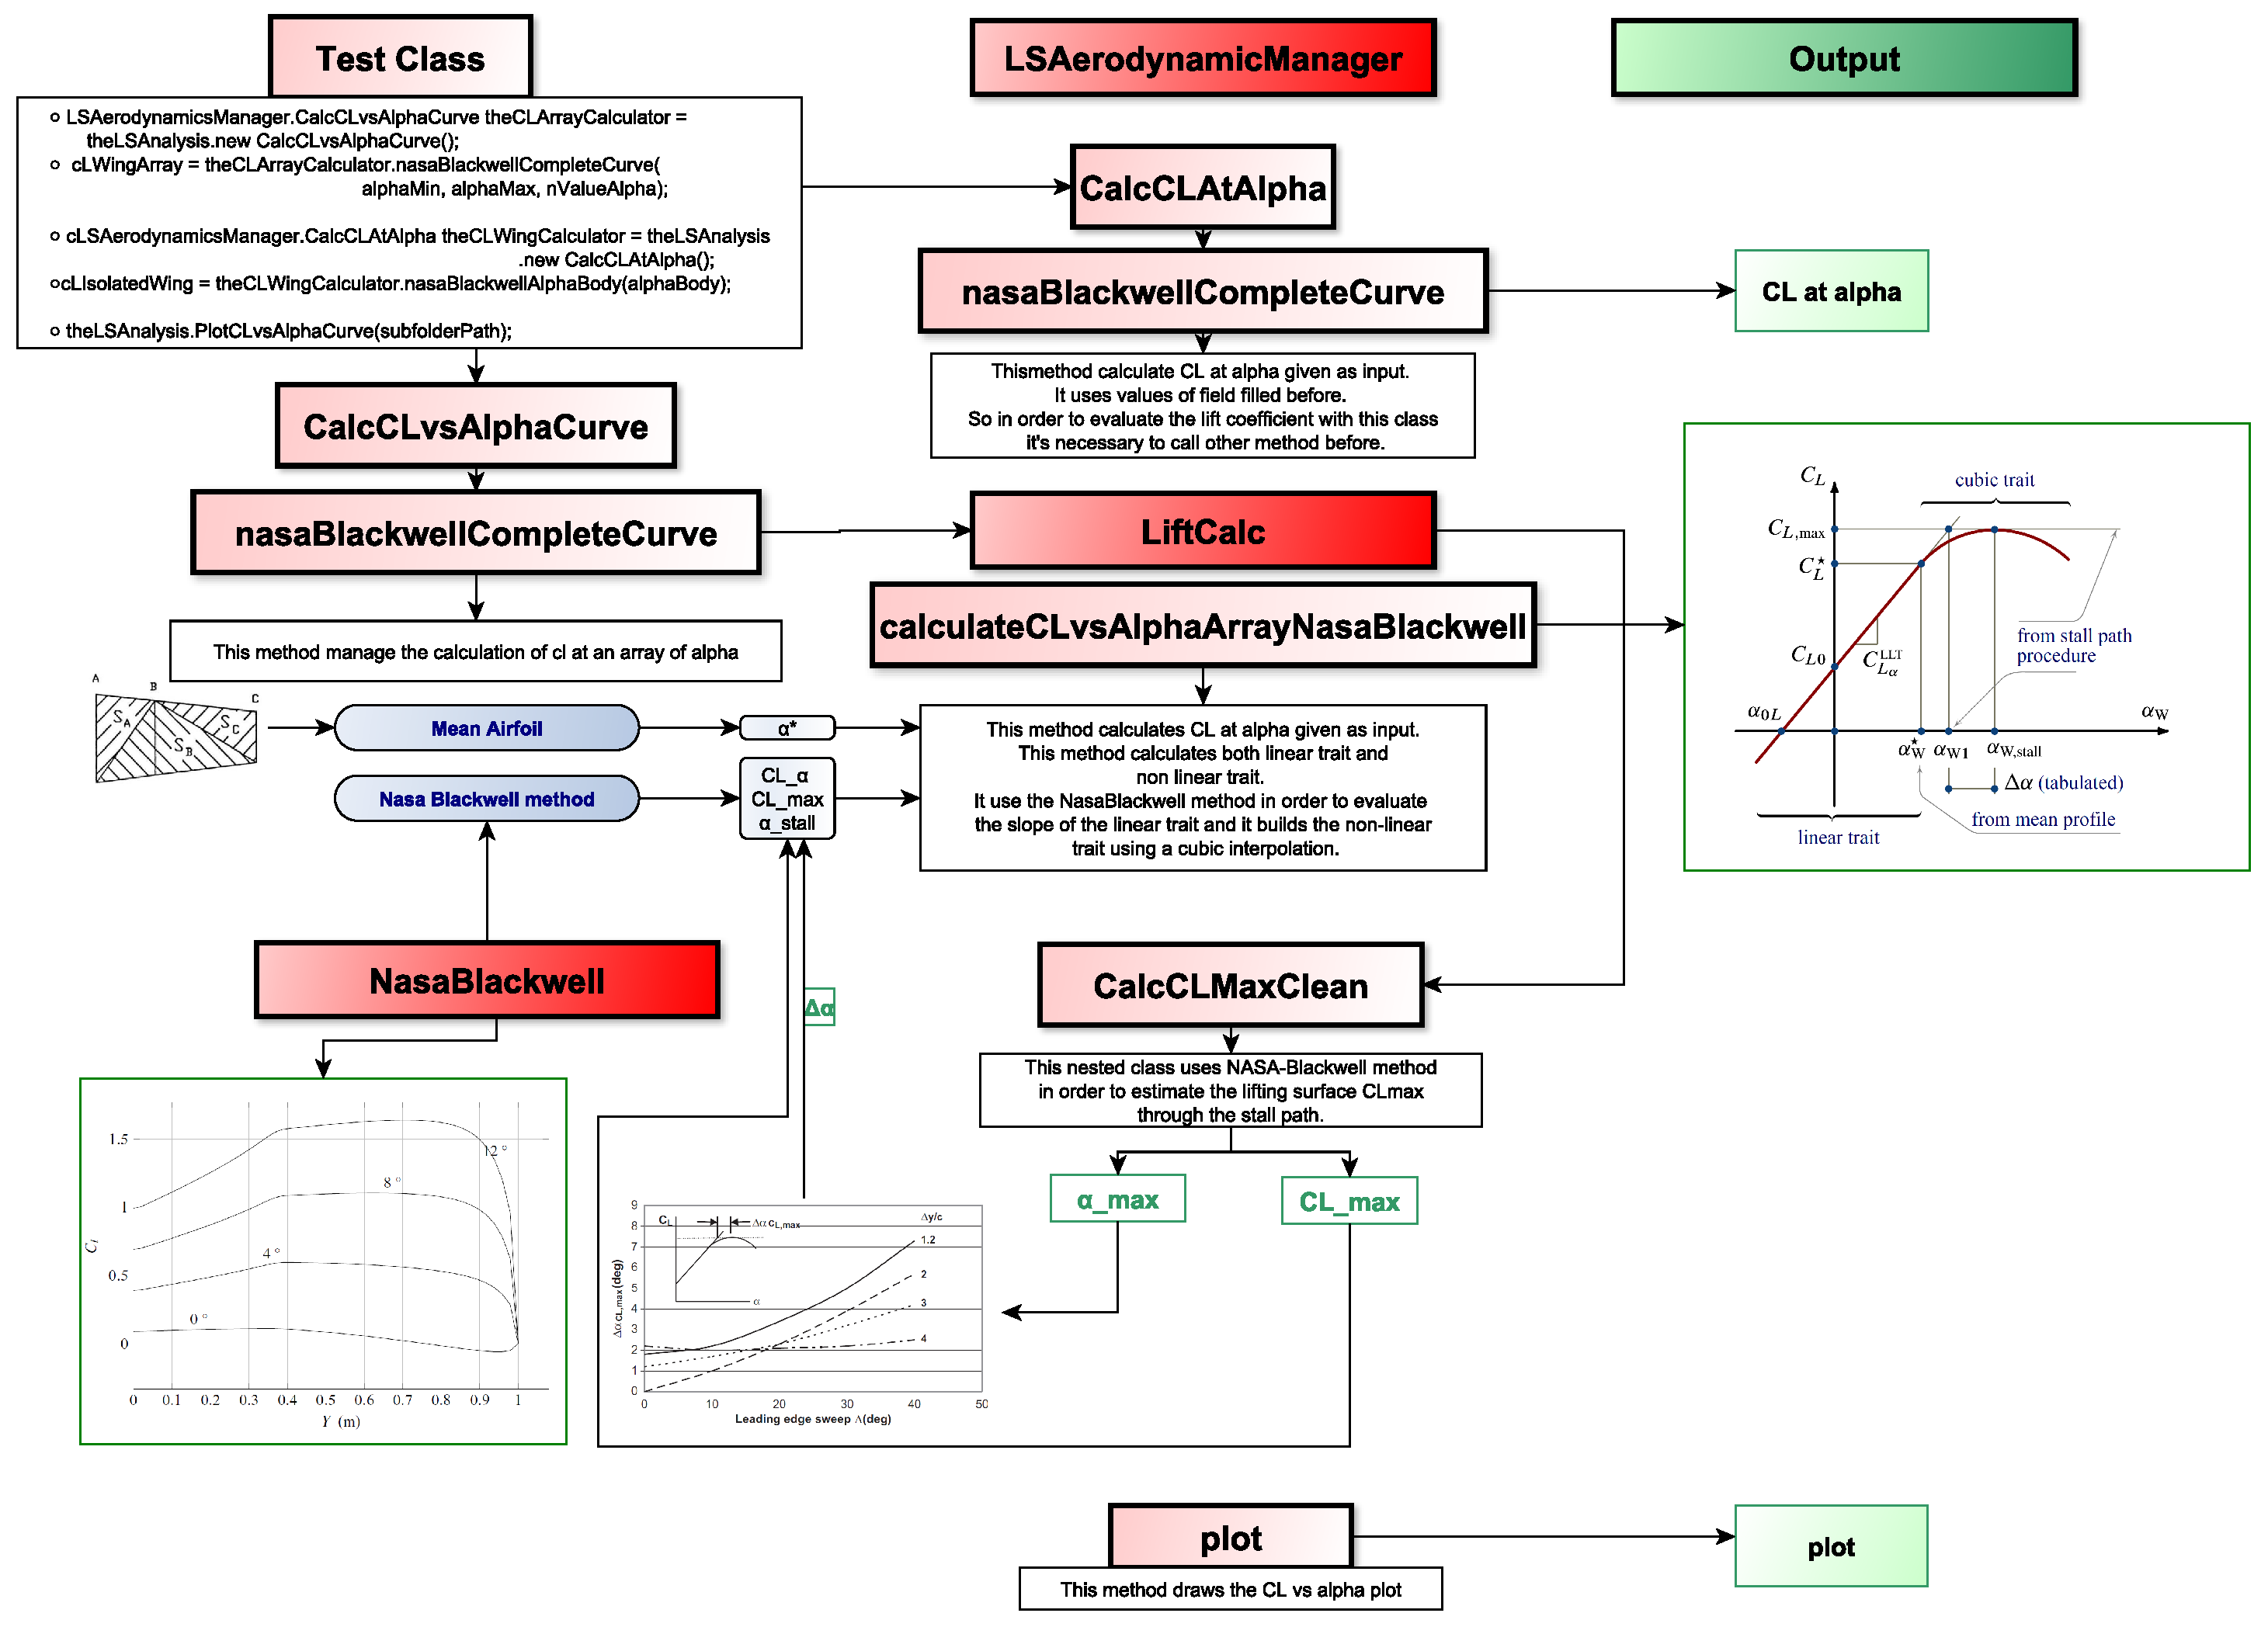
\includegraphics[height=14.6cm, angle=90]{Immagini/clflowchart.pdf}} 
\caption{Flow chart of lift estimation classes.}
\label{fig:clalf}
\end{figure}


\section{Case Study}

The last task to be done is to show an application of the calculation of lift characteristics of a lifting surface in order to validate the calculation performed as well as to give a useful example of use. In previous chapters two aircraft were introduced: ATR-72 and B747-100B. On these two aircrafts analyses were made, the results of which are shown below.\\

\subsection{ATR-72}

In order to correctly use the lift modulus of JPAD it is necessary to set the correct Reynolds number of airfoils and, consequently, the correct value of $CL_{MAX}$. Referring to \cite{Abbott} the value for ATR 72 are the following

\begin{center}
\captionof{table}{Airfoils $CL_{MAX}$ for ATR-72. Mach number = 0.4}
	\begin{tabular}{ | l | l | l | l |}
		\hline
		Station & Airfoil & Reynolds Number & $CL_{max}$ \\ \hline
		Root & NACA 23018 & $6.28 \cdot 10^6$ & 1.65 \\ \hline
		Kink & NACA 23018 &  $6.28 \cdot 10^6$ & 1.65 \\ \hline
		Tip & NACA 23015 & $4.41 \cdot 10^6$ & 1.7 \\
		\hline
	\end{tabular}
\end{center}


\begin{figure}[H]
	\centering
	{\includegraphics[height=6.8cm]{Immagini/ATR_Topview.pdf}} 
	\caption{Lift curve for ATR-72 airfoils and wing for M=0.2.}
	\label{fig:clalf}
\end{figure}

\begin{lstlisting}[frame=rbl,caption={{\footnotesize Lift Characteristics of a Lifting Surface - Test Class}},label= [style=\bfseries]{Listing}]

System.out.println("\n\n------------------------------------");
System.out.println("\n LIFT CHARACTERISTICS  ");
System.out.println("\n------------------------------------");


System.out.println("\n ------------------- ");
System.out.println("|       WING        |");
System.out.println(" ------------------- \n\n");

System.out.println("\n \t Data: ");

System.out.println("Angle of attack alpha body (deg) = "
		+ "" + Math.ceil(alphaBody.to(NonSI.DEGREE_ANGLE)
				.getEstimatedValue()));
System.out.println("Angle of incidence of wing (deg) = "
		+ "" +  Math.ceil(theWing.get_iw()
				.to(NonSI.DEGREE_ANGLE)
				.getEstimatedValue()));

System.out.println("\n \n-----------------------------------------------------");
System.out.println("Starting evaluate stall path of wing");
System.out.println("-----------------------------------------------------");

LSAerodynamicsManager theLSAnalysis = new LSAerodynamicsManager(
				theConditions,
				theWing,
				aircraft
				);
				
LSAerodynamicsManager.CalcCLAtAlpha theCLWingCalculator = 
				theLSAnalysis
				.new CalcCLAtAlpha();
cLIsolatedWing = theCLWingCalculator.nasaBlackwellalphaBody(alphaBody);

theLSAnalysis.PlotCLvsAlphaCurve(subfolderPath);
System.out.println("-------------------------------------");
System.out.println("CL of Isolated wing at alpha body = " + cLIsolatedWing);
System.out.println("\n \t \t \tDONE PLOTTING CL VS ALPHA CURVE  ");

// -----------------------------------------------------------------------
// Using NASA-Blackwell method in order to estimate the lifting surface CLmax
// -----------------------------------------------------------------------


LSAerodynamicsManager.CalcCLMaxClean theCLmaxAnalysis = 
		theLSAnalysis
		.new CalcCLMaxClean(); //is nested
LSAerodynamicsManager.CalcCLvsAlphaCurve theCLAnalysis
       = theLSAnalysis.new CalcCLvsAlphaCurve();
theCLAnalysis.nasaBlackwell();
theCLmaxAnalysis.nasaBlackwell();
Amount<Angle> alphaAtCLMax = theLSAnalysis.get_alphaStall();
double clMax = theCLWingCalculator.nasaBlackwell(alphaAtCLMax);


// PLOT

System.out.println("\n \n \t \t WRITING CHART TO FILE. Stall path. ");

// interpolation of CL MAX_airfoil
		MyArray clMaxAirfoil = theCLmaxAnalysis.getClAirfoils();

		MyArray clAlphaThird = theLSAnalysis.getcLMap()
				.getCxyVsAlphaTable()
				.get(MethodEnum.NASA_BLACKWELL ,alphaAtCLMax);

		double [][] semiSpanAd = {
				theLSAnalysis.get_yStationsND(),
				 theLSAnalysis.get_yStationsND()};

		double [][] clDistribution = {
				clMaxAirfoil.getRealVector().toArray(), 
				clAlphaThird.getRealVector().toArray()};
		String [] legend = new String [4];
		legend[0] = "CL max airfoil";
		legend[1] = "CL distribution at alpha " 
		+ Math.toDegrees( alphaAtCLMax.getEstimatedValue());


MyChartToFileUtils.plot(
		semiSpanAd,	clDistribution, // array to plot
		0.0, 1.0, 0.0, 2.0,					
		"eta", "CL", "", "",	    // label with unit
		legend,					// legend
		subfolderPath, "Stall Path of Wing ");			


System.out.println("-----------------------------------------------------");
System.out.println("\t \t DONE ");

\end{lstlisting}


\begin{lstlisting}[caption={{\footnotesize Lift Characteristics of a Lifting Surface - Results for M=0.2. ATR-72}},label= [style=\bfseries]{Listing}]
------------------------------------

 LIFT CHARACTERISTICS  

------------------------------------

 ------------------- 
|       WING        |
 ------------------- 
 	 Data: 
Angle of attack alpha body (deg) = 2.0
Angle of incidence of wing (deg) = 2.0

 
-----------------------------------------------------
Starting evaluate stall path of wing
-----------------------------------------------------

 -----------CLEAN-------------- 
 alpha max 15.229385456031025 (deg)
 alpha star 10.918671750781748 (deg)
 cL max 1.4880884199886235
 cL star 1.1785803287397512
 cL alpha 5.582578511036018 (1/rad)
-------------------------------------
CL of Isolated wing at alpha body = 0.5045422247468523

 	 	 	DONE PLOTTING CL VS ALPHA CURVE  

 
 	 	 WRITING CHART TO FILE. Stall path. 
-----------------------------------------------------
	 	 DONE 
\end{lstlisting}


\noindent \\

\begin{figure}[H]
\centering
\input{immagini/stallpathatr.tikz}
\caption{ATR 72 Stall Path of wing at Mach 0.2.}
\label{fig:stallATR}
\end{figure}


\begin{figure}[H]
\centering
%CL vs Alpha clean WING
\begin{tikzpicture}

\begin{axis}[
width=0.85\textwidth,
height=0.75\textwidth,
scaled ticks=false, tick label style={/pgf/number format/fixed},
xmin=-2,
xmax=18,
xlabel={$\alpha_{body}$ (deg)},
xmajorgrids,
ymin=-0.1,
ymax=1.6,
ylabel={$C_L$ },
ymajorgrids,
]

\addplot [
color=black,
thick
]
table[row sep=crcr]{
-10.0	-0.8595390360144025\\
-9.30183939177138	-0.7915141929653783\\
-8.603678783542762	-0.723489349916354\\
-7.905518175314142	-0.6554645068673297\\
-7.207357567085522	-0.5874396638183055\\
-6.509196958856902	-0.519414820769281\\
-5.811036350628282	-0.4513899777202568\\
-5.112875742399662	-0.38336513467123234\\
-4.4147151341710416	-0.3153402916222081\\
-3.716554525942422	-0.24731544857318366\\
-3.0183939177138024	-0.17929060552415943\\
-2.320233309485183	-0.11126576247513506\\
-1.6220727012565632	-0.0432409194261108\\
-0.9239120930279435	0.024783923622913512\\
-0.22575148479932383	0.09280876667193784\\
0.47240912342929586	0.16083360972096217\\
1.1705697316579156	0.22885845276998645\\
1.8687303398865351	0.29688329581901074\\
2.5668909481151547	0.364908138868035\\
3.2650515563437743	0.43293298191705937\\
3.963212164572394	0.5009578249660838\\
4.6613727728010135	0.568982668015108\\
5.3595333810296335	0.6370075110641324\\
6.0576939892582535	0.7050323541131567\\
6.755854597486874	0.773057197162181\\
7.454015205715494	0.8410820402112054\\
8.152175813944114	0.9091068832602297\\
8.850336422172733	0.9771317263092539\\
9.548497030401352	1.0451565693582783\\
10.246657638629971	1.1131814124073025\\
10.94481824685859	1.1812096690481177\\
11.64297885508721	1.250789828512938\\
12.341139463315828	1.31974640200939\\
13.039300071544448	1.3830048566498019\\
13.737460679773067	1.43549065954651\\
14.435621288001686	1.472129277811844\\
15.133781896230305	1.4878461785581298\\
15.831942504458924	1.4775668288977095\\
16.530103112687545	1.436216695942909\\
17.228263720916168	1.3587212468060668\\
};
\end{axis}
\end{tikzpicture}%

\caption{ATR 72 CL vs Alpha_w at Mach 0.2.}
\label{fig:clATR}
\end{figure}

\begin{figure}[H]
\centering
%CL vs Alpha clean WING
\begin{tikzpicture}

\begin{axis}[
width=0.85\textwidth,
height=0.6\textwidth,
scaled ticks=false, tick label style={/pgf/number format/fixed},
xmin=-10,
xmax=18,
xlabel={$\alpha_{body}$ (deg)},
xmajorgrids,
ymin=-0.9,
ymax=1.6,
ylabel={$C_L$ },
ymajorgrids,
legend style={at={(0.6,0.1)},anchor=west,draw=black,fill=white,legend cell align=left},
legend entries = {M=0.4\\M=0.65\\}
]

\addplot [
color=black,
thick
]
table[row sep=crcr]{
-10.0	-0.8492929893620671\\
-9.297278522952698	-0.7816396236505276\\
-8.594557045905397	-0.7139862579389877\\
-7.891835568858096	-0.6463328922274483\\
-7.189114091810795	-0.5786795265159088\\
-6.486392614763495	-0.5110261608043694\\
-5.783671137716194	-0.4433727950928297\\
-5.080949660668893	-0.37571942938129016\\
-4.378228183621593	-0.3080660636697507\\
-3.6755067065742915	-0.24041269795821102\\
-2.9727852295269903	-0.17275933224667145\\
-2.270063752479689	-0.10510596653513188\\
-1.567342275432388	-0.03745260082359231\\
-0.864620798385087	0.030200764887947262\\
-0.16189932133778595	0.09785413059948683\\
0.5408221557095151	0.1655074963110264\\
1.2435436327568161	0.233160862022566\\
1.9462651098041173	0.30081422773410554\\
2.6489865868514184	0.36846759344564517\\
3.3517080638987196	0.43612095915718474\\
4.05442954094602	0.5037743248687243\\
4.757151017993321	0.5714276905802638\\
5.459872495040622	0.6390810562918033\\
6.162593972087922	0.7067344220033429\\
6.865315449135223	0.7743877877148825\\
7.568036926182524	0.8420411534264218\\
8.270758403229825	0.9096945191379616\\
8.973479880277127	0.9773478848495011\\
9.676201357324429	1.0450012505610409\\
10.37892283437173	1.1126546162725803\\
11.081644311419032	1.18043691390843\\
11.784365788466333	1.2503228114740352\\
12.487087265513635	1.319267928049312\\
13.189808742560936	1.3823490591100178\\
13.892530219608238	1.4346430001319082\\
14.59525169665554	1.4712265465907404\\
15.297973173702841	1.48717649396227\\
16.00069465075014	1.4775696377222598\\
16.703416127797443	1.4374827733464635\\
17.40613760484474	1.361992696310633\\
};
\addplot [
color=black,
densely dashed
]
table[row sep=crcr]{
-10.0	-0.9830709498739174\\
-9.353404038062589	-0.9110197055897866\\
-8.706808076125178	-0.8389684613056556\\
-8.060212114187767	-0.7669172170215245\\
-7.413616152250356	-0.6948659727373936\\
-6.7670201903129445	-0.6228147284532626\\
-6.1204242283755335	-0.5507634841691317\\
-5.473828266438122	-0.47871223988500067\\
-4.827232304500711	-0.40666099560086966\\
-4.1806363425633	-0.33460975131673865\\
-3.534040380625889	-0.2625585070326078\\
-2.887444418688478	-0.19050726274847685\\
-2.240848456751067	-0.11845601846434581\\
-1.5942524948136558	-0.04640477418021485\\
-0.9476565328762449	0.025646470103916075\\
-0.30106057093883387	0.09769771438804703\\
0.3455353909985771	0.169748958672178\\
0.9921313529359881	0.24180020295630894\\
1.6387273148733992	0.3138514472404399\\
2.2853232768108103	0.38590269152457085\\
2.9319192387482214	0.4579539358087018\\
3.5785152006856324	0.5300051800928328\\
4.225111162623043	0.6020564243769637\\
4.871707124560454	0.6741076686610947\\
5.518303086497865	0.7461589129452257\\
6.164899048435276	0.8182101572293566\\
6.8114950103726875	0.8902614015134876\\
7.4580909723100985	0.9623126457976184\\
8.104686934247509	1.0343638900817496\\
8.75128289618492	1.1064151343658806\\
9.397878858122331	1.1784663786500114\\
10.044474820059742	1.2505176229341421\\
10.691070781997153	1.3225688672182734\\
11.337666743934564	1.390505200152445\\
11.984262705871975	1.439904417061328\\
12.630858667809386	1.4691032486904354\\
13.277454629746797	1.4776297707703807\\
13.924050591684209	1.4650120590317752\\
14.57064655362162	1.4307781892052334\\
15.217242515559029	1.3744562370213669\\
};
\end{axis}
\end{tikzpicture}%

\caption{ATR-72 lift curve. Variation with Mach number.}
\label{fig:clATR}
\end{figure}




\begin{center}
\captionof{table}{High-lift devices geometrical data for ATR72}
	\begin{tabular}{| l | l | l | l | l |}
	\hline
		 Number of Flap & Type &  $\eta$ in &  $\eta$ out &   $\frac{c_{f}}{c} $   \\ \hline
		1  & Single Slotted& 0.08  & 0.35 &  0.38 \\ \hline
		2  & Single Slotted& 0.35 & 0.8 & 0.38 \\ \hline
		\hline
	\end{tabular}
\end{center}


\begin{center}
\captionof{table}{High-lift devices data for ATR72}
	\begin{tabular}{ | l | l | l |}
		\hline
		Configuration &  $\delta_{f_1}$ & $\delta_{f_2}$  \\ \hline
		Take off &  $22^{\circ}$ &  $22^{\circ}$\\ \hline
		Landing  &  $40^{\circ}$ &  $40^{\circ}$\\ \hline
		\hline
	\end{tabular}
\end{center}



\begin{figure}[H]
\centering
%CL alpha Wing High Lift
\begin{tikzpicture}

\begin{axis}[
width=0.9\textwidth,
height=0.55\textheight,
scaled ticks=false, tick label style={/pgf/number format/fixed},
xmin=-14.0,
xmax=20,
xlabel={alpha ($\deg$)},
xmajorgrids,
ymin=-0.8595390360144025,
ymax=2.7,
ylabel={C\textsubscript{L}},
ymajorgrids,
legend entries = {Clean\\Flap@TO\\}
]

\addplot [
color=black,
densely dashed
]
table[row sep=crcr]{
-10.0	-0.7990169022409647\\
-9.244265130095556	-0.730565177361426\\
-8.488530260191112	-0.662113452481887\\
-7.732795390286668	-0.5936617276023484\\
-6.977060520382224	-0.5252100027228094\\
-6.22132565047778	-0.4567582778432707\\
-5.465590780573336	-0.38830655296373184\\
-4.709855910668892	-0.319854828084193\\
-3.9541210407644485	-0.2514031032046542\\
-3.1983861708600045	-0.18295137832511532\\
-2.4426513009555606	-0.11449965344557647\\
-1.6869164310511167	-0.04604792856603768\\
-0.9311815611466728	0.022403796313501145\\
-0.175446691242229	0.09085552119303995\\
0.5802881786622148	0.1593072460725788\\
1.3360230485666587	0.2277589709521176\\
2.0917579184711026	0.29621069583165643\\
2.8474927883755465	0.36466242071119526\\
3.6032276582799905	0.4331141455907341\\
4.358962528184434	0.5015658704702729\\
5.114697398088878	0.5700175953498117\\
5.870432267993322	0.6384693202293504\\
6.626167137897766	0.7069210451088894\\
7.38190200780221	0.7753727699884282\\
8.137636877706653	0.843824494867967\\
8.893371747611097	0.912276219747506\\
9.64910661751554	0.9807279446270446\\
10.404841487419985	1.0491796695065831\\
11.160576357324429	1.118003287133353\\
11.916311227228872	1.1913380917053247\\
12.672046097133316	1.2675498588842884\\
13.42778096703776	1.3430685741896835\\
14.183515836942204	1.4143242231409459\\
14.939250706846648	1.4777467912575113\\
15.694985576751092	1.5297662640588183\\
16.450720446655534	1.5668126270643028\\
17.20645531655998	1.5853158657934023\\
17.962190186464422	1.5817059657655537\\
18.717925056368866	1.5524129125001962\\
19.47365992627331	1.4938666915167658\\
};

\addplot [
color=black,
solid
]
table[row sep=crcr]{
-13.0	-0.2097986399387466\\
-12.335985442698906	-0.14899594705625985\\
-11.671970885397812	-0.08819325417377333\\
-11.007956328096718	-0.027390561291286808\\
-10.343941770795624	0.03341213159119971\\
-9.67992721349453	0.09421482447368634\\
-9.015912656193436	0.15501751735617308\\
-8.351898098892342	0.2158202102386595\\
-7.687883541591248	0.27662290312114624\\
-7.023868984290154	0.33742559600363276\\
-6.35985442698906	0.3982282888861193\\
-5.6958398696879655	0.4590309817686059\\
-5.0318253123868715	0.5198336746510924\\
-4.367810755085777	0.5806363675335792\\
-3.7037961977846834	0.6414390604160657\\
-3.0397816404835893	0.7022417532985523\\
-2.3757670831824953	0.7630444461810388\\
-1.7117525258814013	0.8238471390635254\\
-1.0477379685803072	0.8846498319460121\\
-0.38372341127921306	0.9454525248284986\\
0.2802911460218811	1.0062552177109851\\
0.9443057033229753	1.0670579105934719\\
1.6083202606240694	1.1278606034759584\\
2.2723348179251635	1.188663296358445\\
2.9363493752262575	1.2494659892409317\\
3.6003639325273515	1.3102686821234182\\
4.264378489828446	1.3710713750059047\\
4.92839304712954	1.4318740678883914\\
5.592407604430634	1.492676760770878\\
6.256422161731728	1.5534774880447664\\
6.920436719032822	1.6140771803668772\\
7.584451276333916	1.673915330814697\\
8.248465833635011	1.7323928453851856\\
8.912480390936105	1.7889106300753017\\
9.5764949482372	1.8428695908820059\\
10.240509505538293	1.8936706338022566\\
10.904524062839387	1.9407146648330142\\
11.568538620140481	1.983402589971238\\
12.232553177441575	2.021135315213887\\
12.89656773474267	2.0533137465579214\\
13.560582292043764	2.0793387900003\\
14.224596849344858	2.0986113515379827\\
14.888611406645952	2.1105323371679297\\
15.552625963947046	2.114502652887099\\
16.21664052124814	2.1099232046924508\\
16.880655078549236	2.096194898580945\\
17.54466963585033	2.0727186405495406\\
18.208684193151424	2.038895336595197\\
18.872698750452518	1.9941258927148748\\
19.536713307753615	1.937811214905532\\
};
\end{axis}
\end{tikzpicture}%

\caption{ATR-72 lift curve with and without flaps in take-off configuration.}
\label{fig:clATR}
\end{figure}


\begin{lstlisting}[caption={{\footnotesize Wing Lift characteristic results for TAKE-OFF. ATR-72, M=0.2 }},label= [style=\bfseries]{Listing}]

 -----------CLEAN-------------- 
 alpha max 17.8116610484647 (deg)
 alpha star 9.6267723716381 (deg)
 cl max 1.5370911540497318
 cl star 0.9854862505109439
 cl alpha 5.227776418346189 (1/rad)

 ----------- DELTA HIGH LIFT TAKE_OFF-------------- 
deltaCL0_flap = 0.80887111935885
deltaCLmax_flap = 0.6053024400694088
deltaCLmax_slat = 0.0
cLalpha_new = (1/rad) 5.26834311032201
deltaAlphaMax = (deg) 2.139367521679026
deltaCD = 0.022631019249350154
deltaCMc_4 = -0.14067311296011697

-----------HIGH LIFT-------------- 
 alpha max 15.47805767446944 (deg)
 alpha star 5.191658954896691 (deg)
 cl max 2.1423935941191408
 cl star 1.393329795148776
 cl alpha 5.26834311032201 (1/rad)


CL wing TAKE_OFF Array [0.594167494459124, 0.6448337842917097, 0.6955000741242955...]

CL of wing at TAKE_OFF at alpha body = 1.2378170282582692

\end{lstlisting}


\subsection{BOEING 747-100B}

\begin{figure}[H]
	\centering
	{\includegraphics[height=6.9cm]{Immagini/BOEING_Topview.pdf}} 
	\caption{Lift curve for BOEING 747-100B similar airfoils and wing.}
	\label{fig:clalf}
\end{figure}

\begin{center}
\captionof{table}{Airfoils $CL_{MAX}$ for BOEING 747-100B. Mach number = 0.84}
	\begin{tabular}{ | l | l | l | l |}
		\hline
		Station & Airfoil & Reynolds Number & $CL_{max}$ \\ \hline
		Root & similar to BAC root 747 & $3.67 \cdot 10^7$ & 1.7 \\ \hline
		Kink & similar to BAC kink 747 &  $2.18 \cdot 10^7$ & 1.73 \\ \hline
		Tip & similar to BAC tip 747 & $9.53 \cdot 10^6$ & 1.82 \\
		\hline
	\end{tabular}
\end{center}



\begin{lstlisting}[caption={{\footnotesize Lift Characteristics of a Lifting Surface - Results. BOEING 747-100B for M=0.84}},label= [style=\bfseries]{Listing}]
------------------------------------

 LIFT CHARACTERISTICS  

------------------------------------

 ------------------- 
|       WING        |
 ------------------- 


	 Data: 
Angle of incidence of wing (deg) = 1.500110492089126
Angle of attack alpha body (deg) = 2.000147322785501
Angle of attack alpha Wing (deg) = 3.4999999999999996

 -----------CLEAN-------------- 
 alpha max 15.632268822248909 (deg)
 alpha star 9.749010907718121 (deg)
 cL max 1.3961111386040277
 cL star 1.0698441603187268
 cL alpha 5.4275479968166955 (1/rad)



CL wing Clean Array [-0.18514784517157623, -0.12715075362802075, ...]

CL of Isolated wing at alpha body = 0.4779522348097419

-------------------------------------
	 	 	WRITING CL vs ALPHA CHART TO FILE  
	 	 	DONE  

-------------------------------------
	 	 	WRITING STALL PATH CHART TO FILE  
	 	 	DONE  

\end{lstlisting}


\begin{figure}[H]
\centering
%Stall Path of Wing 

\begin{tikzpicture}
\begin{axis}[
width=15.6cm,
height=11cm,
scaled ticks=false, tick label style={/pgf/number format/fixed},
xmin=0,
xmax=1,
xlabel={$\eta$},
xmajorgrids,
ymin=0,
ymax=2.5,
ylabel={$C_L$ },
ymajorgrids,
legend style={at={(0.03,0.86)},anchor=west,draw=black,fill=white,legend cell align=left},
legend entries = {Airfoil $C_{l_{max}}$ distribution\\$C_L$ distribution at $\alpha = 4.5^{\circ}$\\$C_L$ distribution at $\alpha = 11^{\circ}$\\$C_L$ distribution at $\alpha_{max} = 15.67^{\circ}$\\}
]

\addplot [
color=black,
thick
]
table[row sep=crcr]{
0.0	1.7\\
0.02040816326530612	1.7014205218050096\\
0.04081632653061224	1.7028410436100194\\
0.061224489795918366	1.704261565415029\\
0.08163265306122448	1.705682087220039\\
0.1020408163265306	1.7071026090250485\\
0.12244897959183672	1.7085231308300581\\
0.14285714285714285	1.709943652635068\\
0.16326530612244897	1.7113641744400776\\
0.18367346938775508	1.7127846962450872\\
0.2040816326530612	1.714205218050097\\
0.22448979591836732	1.7156257398551067\\
0.24489795918367344	1.7170462616601165\\
0.26530612244897955	1.7184667834651262\\
0.2857142857142857	1.7198873052701358\\
0.30612244897959184	1.7213078270751456\\
0.326530612244898	1.7227283488801552\\
0.34693877551020413	1.724148870685165\\
0.3673469387755103	1.7255693924901747\\
0.3877551020408164	1.7269899142951843\\
0.40816326530612257	1.7284104361001942\\
0.4285714285714287	1.7298309579052038\\
0.44897959183673486	1.7328438721710124\\
0.469387755102041	1.7360718769054195\\
0.48979591836734715	1.7392998816398264\\
0.5102040816326533	1.7425278863742333\\
0.5306122448979594	1.7457558911086404\\
0.5510204081632656	1.7489838958430473\\
0.5714285714285717	1.7522119005774541\\
0.5918367346938779	1.7554399053118612\\
0.612244897959184	1.758667910046268\\
0.6326530612244902	1.761895914780675\\
0.6530612244897963	1.765123919515082\\
0.6734693877551025	1.768351924249489\\
0.6938775510204086	1.7715799289838958\\
0.7142857142857147	1.774807933718303\\
0.7346938775510209	1.7780359384527098\\
0.755102040816327	1.7812639431871167\\
0.7755102040816332	1.7844919479215238\\
0.7959183673469393	1.7877199526559306\\
0.8163265306122455	1.7909479573903375\\
0.8367346938775516	1.7941759621247446\\
0.8571428571428578	1.7974039668591515\\
0.8775510204081639	1.8006319715935584\\
0.89795918367347	1.8038599763279655\\
0.9183673469387762	1.8070879810623723\\
0.9387755102040823	1.8103159857967792\\
0.9591836734693885	1.8135439905311863\\
0.9795918367346946	1.8167719952655932\\
1.0	1.82\\
};

\addplot [
color=black,
densely dashed
]
table[row sep=crcr]{
0.0	0.39487061827282127\\
0.02040816326530612	0.39911705074252873\\
0.04081632653061224	0.4076541258079028\\
0.061224489795918366	0.41652952400519516\\
0.08163265306122448	0.42565594056919437\\
0.1020408163265306	0.4350003715755874\\
0.12244897959183672	0.44457321126375693\\
0.14285714285714285	0.4543740957294088\\
0.16326530612244897	0.46437786597084324\\
0.18367346938775508	0.4745701097074242\\
0.2040816326530612	0.48494953743854413\\
0.22448979591836732	0.4955213181335934\\
0.24489795918367344	0.5062955525015271\\
0.26530612244897955	0.5172869240067404\\
0.2857142857142857	0.5285149938673958\\
0.30612244897959184	0.5400050288788901\\
0.326530612244898	0.5517894134592906\\
0.34693877551020413	0.5639098643385002\\
0.3673469387755103	0.5764209996551953\\
0.3877551020408164	0.5893967448495923\\
0.40816326530612257	0.6029449006401062\\
0.4285714285714287	0.6145161592513364\\
0.44897959183673486	0.6254249790597856\\
0.469387755102041	0.633360562131451\\
0.48979591836734715	0.6413115057499875\\
0.5102040816326533	0.6493898133875153\\
0.5306122448979594	0.6575566546342706\\
0.5510204081632656	0.6657789548369978\\
0.5714285714285717	0.6740253658806955\\
0.5918367346938779	0.682261993141658\\
0.612244897959184	0.6904498113390178\\
0.6326530612244902	0.6985419656814726\\
0.6530612244897963	0.7064805797604713\\
0.6734693877551025	0.7141927071772669\\
0.6938775510204086	0.7215849857301082\\
0.7142857142857147	0.728536392336933\\
0.7346938775510209	0.734888230846914\\
0.755102040816327	0.740430060576933\\
0.7755102040816332	0.7448795946827579\\
0.7959183673469393	0.747853493711417\\
0.8163265306122455	0.7488241422070676\\
0.8367346938775516	0.7470543487497322\\
0.8571428571428578	0.7414963360881737\\
0.8775510204081639	0.7306311355089603\\
0.89795918367347	0.7122047016299027\\
0.9183673469387762	0.6827747555161765\\
0.9387755102040823	0.6368610861589308\\
0.9591836734693885	0.5649379181298013\\
0.9795918367346946	0.44611515170767324\\
1.0	0.0\\
};

\addplot [
color=black,
dashdotted
]
table[row sep=crcr]{
0.0	0.8387947494521667\\
0.02040816326530612	0.8477767439293765\\
0.04081632653061224	0.8657973942499728\\
0.061224489795918366	0.8844589719269927\\
0.08163265306122448	0.9035670678750508\\
0.1020408163265306	0.9230351964868024\\
0.12244897959183672	0.9428455938058949\\
0.14285714285714285	0.9629840168878613\\
0.16326530612244897	0.9834203626599899\\
0.18367346938775508	1.0041413611645198\\
0.2040816326530612	1.0251513942646675\\
0.22448979591836732	1.046465039224036\\
0.24489795918367344	1.0681052719780921\\
0.26530612244897955	1.0901032642282826\\
0.2857142857142857	1.112499212004902\\
0.30612244897959184	1.135344113861151\\
0.326530612244898	1.1587026503714362\\
0.34693877551020413	1.1826576176874466\\
0.3673469387755103	1.207317018935464\\
0.3877551020408164	1.2328267717969783\\
0.40816326530612257	1.259399727792534\\
0.4285714285714287	1.2816993964991628\\
0.44897959183673486	1.3024481469973197\\
0.469387755102041	1.3168656118879882\\
0.48979591836734715	1.3312017497867599\\
0.5102040816326533	1.3456970300647029\\
0.5306122448979594	1.3602760235105569\\
0.5510204081632656	1.3748752582689432\\
0.5714285714285717	1.3894335435808827\\
0.5918367346938779	1.4038844618781028\\
0.612244897959184	1.4181512936094274\\
0.6326530612244902	1.4321417114914776\\
0.6530612244897963	1.4457414990656257\\
0.6734693877551025	1.4588065789583415\\
0.6938775510204086	1.4711524819152604\\
0.7142857142857147	1.48254007076325\\
0.7346938775510209	1.4926558088105895\\
0.755102040816327	1.5010840253965239\\
0.7755102040816332	1.5072672926971142\\
0.7959183673469393	1.510448850764639\\
0.8163265306122455	1.5095873928752164\\
0.8367346938775516	1.5032283128573634\\
0.8571428571428578	1.4893045161105871\\
0.8775510204081639	1.4648196575519261\\
0.89795918367347	1.4253275780858976\\
0.9183673469387762	1.364038135657163\\
0.9387755102040823	1.2701398312480672\\
0.9591836734693885	1.1248328548451343\\
0.9795918367346946	0.8868495822581037\\
1.0	0.0\\
};

\addplot [
color=black,
dashed
]
table[row sep=crcr]{
0.0	1.0000640627321633\\
0.02040816326530612	1.010766398094911\\
0.04081632653061224	1.0322322534886936\\
0.061224489795918366	1.0544489666798336\\
0.08163265306122448	1.0771832195916318\\
0.1020408163265306	1.10032909772408\\
0.12244897959183672	1.1238586077762809\\
0.14285714285714285	1.1477524648087052\\
0.16326530612244897	1.171978769660344\\
0.18367346938775508	1.1965246673579184\\
0.2040816326530612	1.2213966000647827\\
0.22448979591836732	1.2466125629014233\\
0.24489795918367344	1.272200209131688\\
0.26530612244897955	1.29819670032439\\
0.2857142857142857	1.3246497287501686\\
0.30612244897959184	1.3516196408273637\\
0.326530612244898	1.3791828497184266\\
0.34693877551020413	1.4074370749587437\\
0.3673469387755103	1.436509713439624\\
0.3877551020408164	1.4665728362739583\\
0.40816326530612257	1.4978774579690017\\
0.4285714285714287	1.5240745569055993\\
0.44897959183673486	1.5483979697246268\\
0.469387755102041	1.5651701807448557\\
0.48979591836734715	1.5818259400032437\\
0.5102040816326533	1.598652386123212\\
0.5306122448979594	1.6155607942351458\\
0.5510204081632656	1.63247664975008\\
0.5714285714285717	1.6493279206360283\\
0.5918367346938779	1.6660363743487638\\
0.612244897959184	1.6825115977154743\\
0.6326530612244902	1.698644744149018\\
0.6530612244897963	1.714301129906951\\
0.6734693877551025	1.7293108370663106\\
0.6938775510204086	1.7434562988887734\\
0.7142857142857147	1.7564554695665604\\
0.7346938775510209	1.767938561742706\\
0.755102040816327	1.777415348553641\\
0.7755102040816332	1.7842284486163926\\
0.7959183673469393	1.7874854453191305\\
0.8163265306122455	1.7859584175320053\\
0.8367346938775516	1.7779321357558397\\
0.8571428571428578	1.7609692065093554\\
0.8775510204081639	1.7315365815753476\\
0.89795918367347	1.6843917480484274\\
0.9183673469387762	1.6115283479740061\\
0.9387755102040823	1.5001981253624803\\
0.9591836734693885	1.3282321873237517\\
0.9795918367346946	1.046960137106503\\
1.0	0.0\\
};
\end{axis}
\end{tikzpicture}%

\caption{BOEING 747-100B Stall Path at Mach 0.84.}
\label{fig:stallB}
\end{figure}


\begin{center}
\captionof{table}{High-lift devices geometrical data for BOEING 747-100B. Flap.}
	\begin{tabular}{| l | l | l | l | l |}
		\hline
		 Number of Flap & Type &  $\eta$ in &  $\eta$ out &   $\frac{c_{f}}{c} $  \\ \hline
				1  & Triple Slotted&  0.104  & 0.357  & 0.18 \\ \hline 
		         2& Triple Slotted & 0.411 & 0.636 &0.18\\ \hline 
		\hline
	\end{tabular}
\end{center}


\begin{center}
\captionof{table}{High-lift devices geometrical data for BOEING 747-100B. Slat.}
	\begin{tabular}{| l | l | l | l | l |}
		\hline
		 Number of Slat &  $\eta$ in &  $\eta$ out &   $\frac{c_{ext}}{c} $ & $\frac{c_{s}}{c} $   \\ \hline
				1 & 0.192  & 0.364  &1.1 & 0.09\\ \hline 
		         2 & 0.414  & 0.648  &1.1& 0.136\\ \hline 
		         3 & 0.692  & 0.961  &1.1& 0.187\\ \hline 
		\hline
	\end{tabular}
\end{center}


\begin{center}
\captionof{table}{High-lift devices data for  BOEING 747-100B}
	\begin{tabular}{ | l | l | l | l | l | l |}
		\hline
		Configuration &  $\delta_{f_1}$ & $\delta_{f_2}$ &  $\delta_{s_1}$ & $\delta_{s_2}$& $\delta_{s_3}$ \\ \hline
		Take off &  $5^{\circ}$, $3^{\circ}$, $2^{\circ}$ & $5^{\circ}$, $3^{\circ}$, $2^{\circ}$ & $10^{\circ}$ &  $10^{\circ}$ &  $10^{\circ}$\\ \hline
		Landing  &    $10^{\circ}$, $10^{\circ}$, $10^{\circ}$ & $10^{\circ}$, $10^{\circ}$, $10^{\circ}$ & $20^{\circ}$ &  $20^{\circ}$ &  $20^{\circ}$\\ \hline
		\hline
	\end{tabular}
\end{center}


\begin{figure}[H]
\centering
%CL alpha Wing High Lift
\begin{tikzpicture}

\begin{axis}[
width=0.8\textwidth,
height=0.85\textwidth,
scaled ticks=false, tick label style={/pgf/number format/fixed},
xmin=-14.0,
xmax=30,
xlabel={alpha ($\deg$)},
xmajorgrids,
ymin=-0.9,
ymax=2.5,
ylabel={C\textsubscript{L}},
ymajorgrids,
legend entries = {Clean\\Flap+Slat@TO\\}
]

\addplot [
color=black,
densely dashed
]
table[row sep=crcr]{
-10.0	-0.6352658757762881\\
-9.136225640983186	-0.5731327253055505\\
-8.272451281966372	-0.5109995748348128\\
-7.4086769229495575	-0.4488664243640752\\
-6.544902563932743	-0.3867332738933375\\
-5.681128204915928	-0.32460012342259975\\
-4.817353845899113	-0.2624669729518621\\
-3.9535794868822984	-0.2003338224811243\\
-3.0898051278654837	-0.13820067201038666\\
-2.226030768848669	-0.07606752153964896\\
-1.3622564098318544	-0.013934371068911253\\
-0.4984820508150398	0.04819877940182644\\
0.3652923082017747	0.11033192987256413\\
1.2290666672185893	0.17246508034330182\\
2.092841026235404	0.23459823081403952\\
2.956615385252219	0.2967313812847773\\
3.8203897442690335	0.3588645317555149\\
4.684164103285848	0.42099768222625267\\
5.547938462302663	0.4831308326969903\\
6.411712821319478	0.5452639831677281\\
7.275487180336293	0.6073971336384656\\
8.139261539353107	0.6695302841092035\\
9.003035898369921	0.7316634345799412\\
9.866810257386735	0.7937965850506788\\
10.730584616403549	0.8562885913586846\\
11.594358975420363	0.9210695330328473\\
12.458133334437177	0.9874024124846988\\
13.32190769345399	1.0540582567871901\\
14.185682052470804	1.1198080930132723\\
15.049456411487618	1.183422948235896\\
15.913230770504432	1.2436738495280117\\
16.777005129521246	1.2993318239625704\\
17.64077948853806	1.3491678986125228\\
18.504553847554877	1.3919531005508203\\
19.368328206571693	1.4264584568504133\\
20.23210256558851	1.4514549945842523\\
21.095876924605324	1.46571374082529\\
21.95965128362214	1.4680057226464747\\
22.823425642638956	1.4571019671207581\\
23.687200001655764	1.4317735013210915\\
};

\addplot [
color=black,
solid
]
table[row sep=crcr]{
-13.0	-0.6656753795627666\\
-12.147624487600394	-0.6033806637646808\\
-11.295248975200789	-0.5410859479665948\\
-10.442873462801183	-0.4787912321685088\\
-9.590497950401577	-0.416496516370423\\
-8.738122438001971	-0.354201800572337\\
-7.885746925602365	-0.29190708477425126\\
-7.033371413202758	-0.22961236897616527\\
-6.180995900803151	-0.16731765317807928\\
-5.328620388403545	-0.10502293737999341\\
-4.476244876003938	-0.04272822158190742\\
-3.623869363604332	0.019566494216178454\\
-2.771493851204726	0.08186121001426439\\
-1.9191183388051196	0.14415592581235026\\
-1.0667428264055134	0.2064506416104362\\
-0.21436731400590714	0.2687453574085221\\
0.6380081983936992	0.331040073206608\\
1.4903837107933056	0.39333478900469393\\
2.3427592231929117	0.45562950480277986\\
3.195134735592518	0.5179242206008657\\
4.0475102479921246	0.5802189363989516\\
4.899885760391731	0.6425136521970376\\
5.752261272791338	0.7048083679951236\\
6.604636785190944	0.7671030837932096\\
7.457012297590551	0.8293977995912953\\
8.309387809990158	0.8916925153893813\\
9.161763322389763	0.9539872311874671\\
10.01413883478937	1.016281946985553\\
10.866514347188975	1.0785766627836388\\
11.71888985958858	1.1408713785817248\\
12.571265371988186	1.2031660943798108\\
13.423640884387792	1.2654622144570093\\
14.276016396787398	1.3292987998867514\\
15.128391909187004	1.3952270046956958\\
15.98076742158661	1.462047574490369\\
16.833142933986217	1.5285612548772958\\
17.685518446385824	1.5935687914630023\\
18.537893958785432	1.655870929854015\\
19.39026947118504	1.71426841565686\\
20.242644983584647	1.767561994478062\\
21.095020495984254	1.8145524119241483\\
21.947396008383862	1.8540404136016424\\
22.79977152078347	1.884826745117074\\
23.652147033183077	1.9057121520769658\\
24.504522545582685	1.9154973800878456\\
25.356898057982292	1.9129831747562378\\
26.2092735703819	1.8969702816886713\\
27.061649082781507	1.8662594464916673\\
27.914024595181115	1.8196514147717553\\
28.766400107580708	1.7559469321354586\\
};
\end{axis}
\end{tikzpicture}%

\caption{BOEING 747-100B  lift curve with and without flaps in take-off configuration.}
\label{fig:clATR}
\end{figure}

\begin{lstlisting}[caption={{\footnotesize Wing Lift characteristic results for TAKE-OFF. BOEING 747-100B, M=0.2 }},label= [style=\bfseries]{Listing}]


-----------CLEAN-------------- 
 alpha max 21.1765973230843 (deg)
 alpha star 9.7482928348910 (deg)
 cl max 1.4597134105954703
 cl star 0.8130642471456172
 cl alpha 4.121408852511737 (1/rad)


 ----------- DELTA HIGH LIFT TAKE_OFF-------------- 
deltaCL0_flap = 0.5985742466275841
deltaCLmax_flap = 0.6272563565428977
deltaCLmax_slat = 0.0
cLalpha_new = (1/rad) 4.153009870215378
deltaAlphaMax = (deg) 2.4385950909414857
deltaCD = 0.023580578759700432
deltaCMc_4 = -0.12074049808439227


 -----------HIGH LIFT-------------- 
 alpha max 21.431119618227623 (deg)
 alpha star 10.003551951328152 (deg)
 cl max 2.086969767138368
 cl star 1.4354638015005163
 cl alpha 4.153009870215378 (1/rad)
 
 CL of wing at TAKE_OFF at alpha body 2 (deg) = 0.9641157258005986
\end{lstlisting}

\section{Modified Stall Path}

In order to evaluate the lift curve of a wing another method has been implemented. This is a modification of Stall Path Method that uses the Nasa-Blackwell lift distribution also for the non linear trait. As known NB method does not see the viscous phenomena. The modified stall path method is based on the consideration that the lift distribution obtained from Nasa-Blackwell is the distribution that you would get if the airfoil's lift moved along the linear lift curve.\\
The process is the following.

\begin{enumerate}
	\item For each angle of attack the lift distribution using Nasa-Blackwell method has been evaluated
	\item For each of n point along the semi-span the local value of $C_L$ is obtained 
	\item Each of these n points corresponds to an intermediate airfoil with its own lift curve
	\item With the local value of $C_l$  it is possible to enter in the linear lift chart obtaining the angle of attack of the airfoil
	\item Using this angle of attack it is possible to enter in the lift curve of the airfoil and derive the local $C_l$
	\item In this way a new lift distribution is obtained that considers the bidimensional non linearity.
	\item The wing $C_L$ is obtained integrating the new lift distribution.
\end{enumerate}

\begin{figure}[H]
	\centering
	{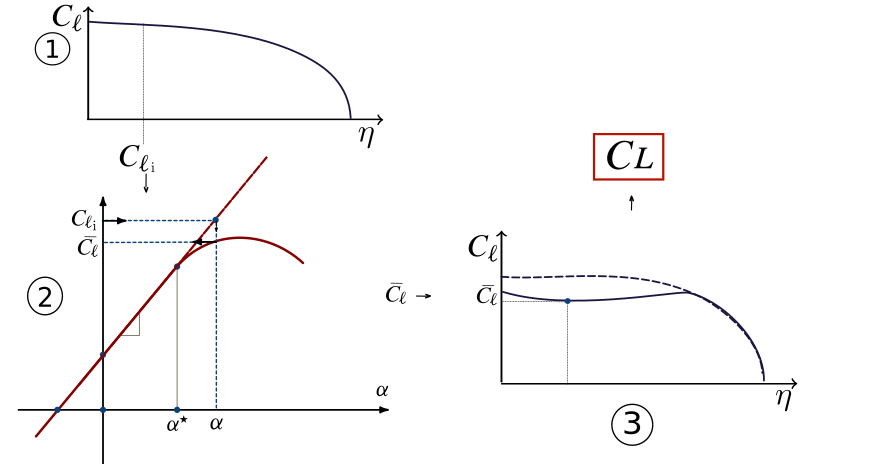
\includegraphics[height=9 cm]{Immagini/stallpathmodified.pdf}} 
	\caption{Flow chart of the modified stall path method.}
	\label{fig:spmm}
\end{figure}

\section{Results Comparison}
In order to compare and validate the results an analysis on a wing has been done with different method.

\begin{center}
\captionof{table}{Airfoils Data}
	\begin{tabular}{| l | l | l | l | l |}
		\hline
		 Station & t/c & $C_{l_{max}}$ & $C_{l_{\alpha}}$ & $\alpha_{stall}$ \\ \hline
		 Root & $0.18$ &  1.90  &  $6.48 (1/rad)$ & $ 18^{\circ} $  \\ \hline
		 Kink & $0.18$ & 1.90  &  $6.48 (1/rad)$ & $ 18^{\circ} $  \\ \hline
		 Tip & $0.18$ &  2.1  &  $6.72 (1/rad)$ & $ 17.5^{\circ} $  \\ \hline
		\hline
	\end{tabular}
\end{center}
\begin{center}
\captionof{table}{Wing Data}
	\begin{tabular}{| l | l | l | l | l |  l |}
		\hline
		  Span & Aspect Ratio & Cr & Ck & Cr & Ad. station kink  \\ \hline
		  31  m & 12 & 2.9 m & 2.9 m & 1.65 m & 0.33\\ \hline
		\hline
	\end{tabular}
\end{center}
\begin{center}
\captionof{table}{Mission Data}
	\begin{tabular}{| l | l |}
		\hline
		  Reynolds Number & Mach Number\\ \hline
		  $13 \cdot 10^6$  & 0.2   \\ \hline
		\hline
	\end{tabular}
\end{center}


The analysis has been done with the following methods :

\begin{itemize}
\item Stall Path
\item Modified Stall Path
\item Philipps and Alley
\item CFD
\end{itemize}

{\bfseries Phillips and Alley} present a method for estimating the maximum wing lift that is based on the classical lifting line theory discussed in Appendix C. Their approach involves providing correction factors for the effects of twist and sweep-back on the span loading of unswept, untwisted, tapered wings. The correction factors are developed with the aid of CFD panel method computations for a variety of conventional wing planforms. Curves for the correction factors are presented for a number of specific taper and aspect ratio as long with the general method for calculating these effects for other wing geometry. \cite{sforza2014commercial}

\begin{equation}
C_{L_{max}} = \left ( \frac{C_L}{c_{l_{max}}}\right)_{\Gamma =0 , \epsilon =0} K_{LS} K_{L\Gamma c_{l_{max}}} \left ( 1 - \frac { K_{L \epsilon} C_{L,\alpha \epsilon}}{c_{l_{max}}} \right) 
\end{equation}

Where $K_{LS}$ is a stall factor

\begin{equation}
K_{LS}=1 + (0.0042 \AR -0.066) \left (1+2.3 \frac{C_{L_{\alpha}}}{ c_{l_{max}}} \right )
\end{equation}

\noindent \\
{\bfseries Computational Fluid Dynamics (CFD)} is a methodology that allows engineers to predict the performance of their designs when exposed to fluid flow, either internal flow (such as the flow of air and gasoline through an engine manifold) or external flow (such as the aerodynamic flow past an automobile or the hydrodynamic flow past a boat). CFD software programs can simulate problems involving gases, liquids and solids and multi-phase problems that depend on the interaction of any number of the above. CFD is used in the design of almost every major product, reducing uncertainty in the design process, and resulting in higher quality products and designs, with greater robustness that better meet customer requirements. CD-adapco is the world's largest independent CFD focused provider of engineering simulation software, support and services. \cite{adapco} \\ \\
Considering the reduction of $CL_{max}$ due to flow separation and other tridimensional effects, an additional modification has been implemented starting from the Stall Path method and the Modified Stall Path Method. The used value for $CL_{max}$ is obtained from the traditional Stall Path method, while the value of $\alpha_{max}$ is obtained from the modified Stall Path Method. In this way a small percentual error has been obtained.


\begin{figure}[H]
	\centering
	{\includegraphics[height=4.9 cm]{Immagini/comparisonairfoil.png}} 
	\caption{Comparison of wing lift curve of airfoils.}
	\label{fig:met}
\end{figure}
	 	 
\noindent \\

	 	 
\begin{figure}[H]
	\centering
	{\includegraphics[height=9.9 cm]{Immagini/clmaxcomparison1.png}} 
	\caption{Comparison of wing lift curve of wing.}
	\label{fig:met}
\end{figure}
	 	 
	 	 
\noindent \\
\begin{center}
\captionof{table}{Lift results comparison}
	\begin{tabular}{| l | l | l | }
		\hline
		 Method  & $C_{L_{MAX}}$ & $\alpha_{stall}$   \\ \hline
		 Stall Path  &1.766  & $17.1 ^{\circ}$  \\ \hline
		 Modified Stall Path  & 1.86   & $19.5^{\circ}$  \\ \hline
		 Modified Stall Path II  & 1.766  & $19.5^{\circ}$  \\ \hline
		 Phillips And Alley  & 1.83  & n.e.\\ \hline
		 CFD  & 1.699  & $19.6 ^{\circ}$   \\ \hline
		\hline
	\end{tabular}
\end{center}

\begin{figure}[H]
	\centering
	{\includegraphics[height=2.63cm]{Immagini/referencepercent.png}} 
	\caption{Percentage Error.}
	\label{fig:met}
\end{figure}


\chapter{Wing Drag Characteristics}

\label{ch:wingdrag}
\markboth{Wing Drag Characteristics}{}

\begin{flushright}
	{\smaller
		\textit{Le avversità\\ possono essere delle formidabili occasioni}\\
		-- Thomas Mann}
\end{flushright}
As mentioned in the previous chapter, the drag is the force component acting in the opposite direction to the airspeed vector.\\
\section{Theoretical background}
There is not a single classification of the drag but, dependent on the purpose of the work, the drag may be broken down in different way. Following will be explained the two main classifications.

\begin{itemize}
\item The drag is subdivided using a causal breakdown. In this way the drag contributes are in accordance with the physical mechanism such as the viscosity of the flow.
\item The drag is subdivided using a component breakdown. Every component of aircraft added an own drag contribute.
\end{itemize}

\begin{figure}[H]
\centering
{\includegraphics[height=6.4cm]{Immagini/component.png}} 
\caption{Drag breakdown for a business jet in cruise.}
\end{figure}
According to the casual breakdown it's possible to make a preliminary division considering normal and tangential stress. The tangential forces produce the {\bfseries friction drag}. While it's possible to divide the drag due of the normal component in viscous, that generates {\bfseries form drag}, and inviscid. A further division can be made for the last one, in {\bfseries induced drag}  and {\bfseries wave drag}.\\
\begin{figure}[H]
\centering
{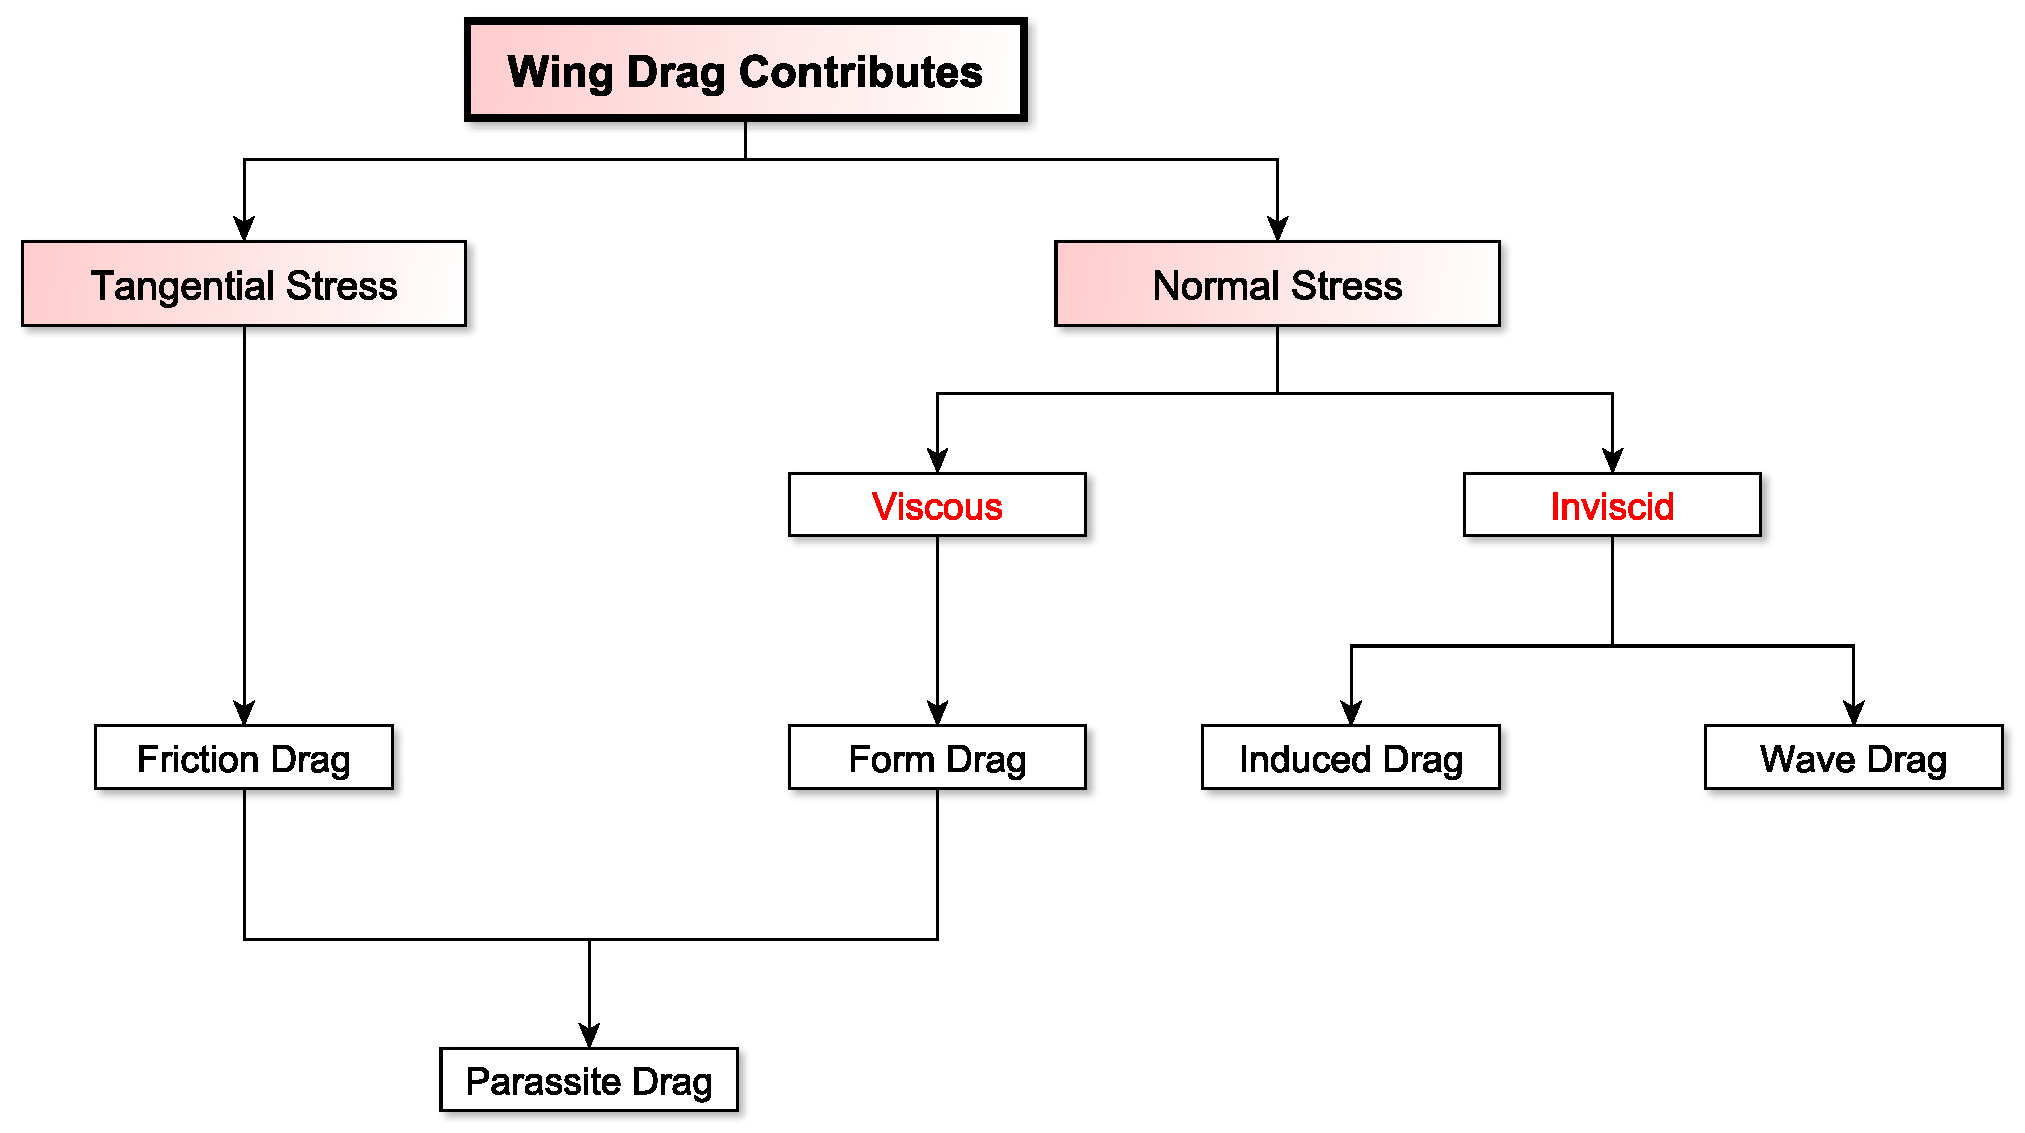
\includegraphics[height=8.9cm]{Immagini/dragcomponentlast.pdf}} 
\caption{Causal breakdown of airplane drags.}
\end{figure}
Friction drag is caused by the air closest to the body’s surface that is dragged along with it. Due to this interaction shearing stresses are born within the thin layer of air (boundary layer) adjacent to the skin. The magnitude of this drag depends on the kind of boundary layer what can be laminar or turbulent in dependence on the Raynolds number. Usually it's accustomed to assume, at the flight speed and altitudes at which aircraft fly, a fully turbulent flow over the entire airplane. In this way a conservative result is obtained.\\
Form drag is caused by the air that is flowing over the body. The separation of air creates turbulence and results in pockets of low and high pressure that leave a wake behind the airplane. The departure of the boundary layer alters the pressure field from its inviscid distribution resulting in an additional drag component. The general size and shape of the body are the most important factors in form drag; bodies with a larger presented cross-section will have a higher drag than thinner bodies.\\
Induced drag is the drag due to lift. It is the drag created by the vortices at the tip of an aircraft's wing. The high pressure underneath the wing causes the airflow at the tips of the wings to curl around from bottom to top in a circular motion. So it's depend on the spanwise distribution of lift. \\
Wave drag is a component of the drag due to the presence of shock waves. Wave drag is independent of viscous effects, and tends to present itself as a sudden and dramatic increase in drag as the vehicle increases speed.
\\ \\ 
In this work the drag will be classified using a component breakdown and for each component of the aircraft is used a causal breakdown. In this way it's possible to evaluate separately the wing drag and tail drag, considering the aerodynamic centers of these lifting surfaces as application point.
\begin{figure}[H]
\centering
{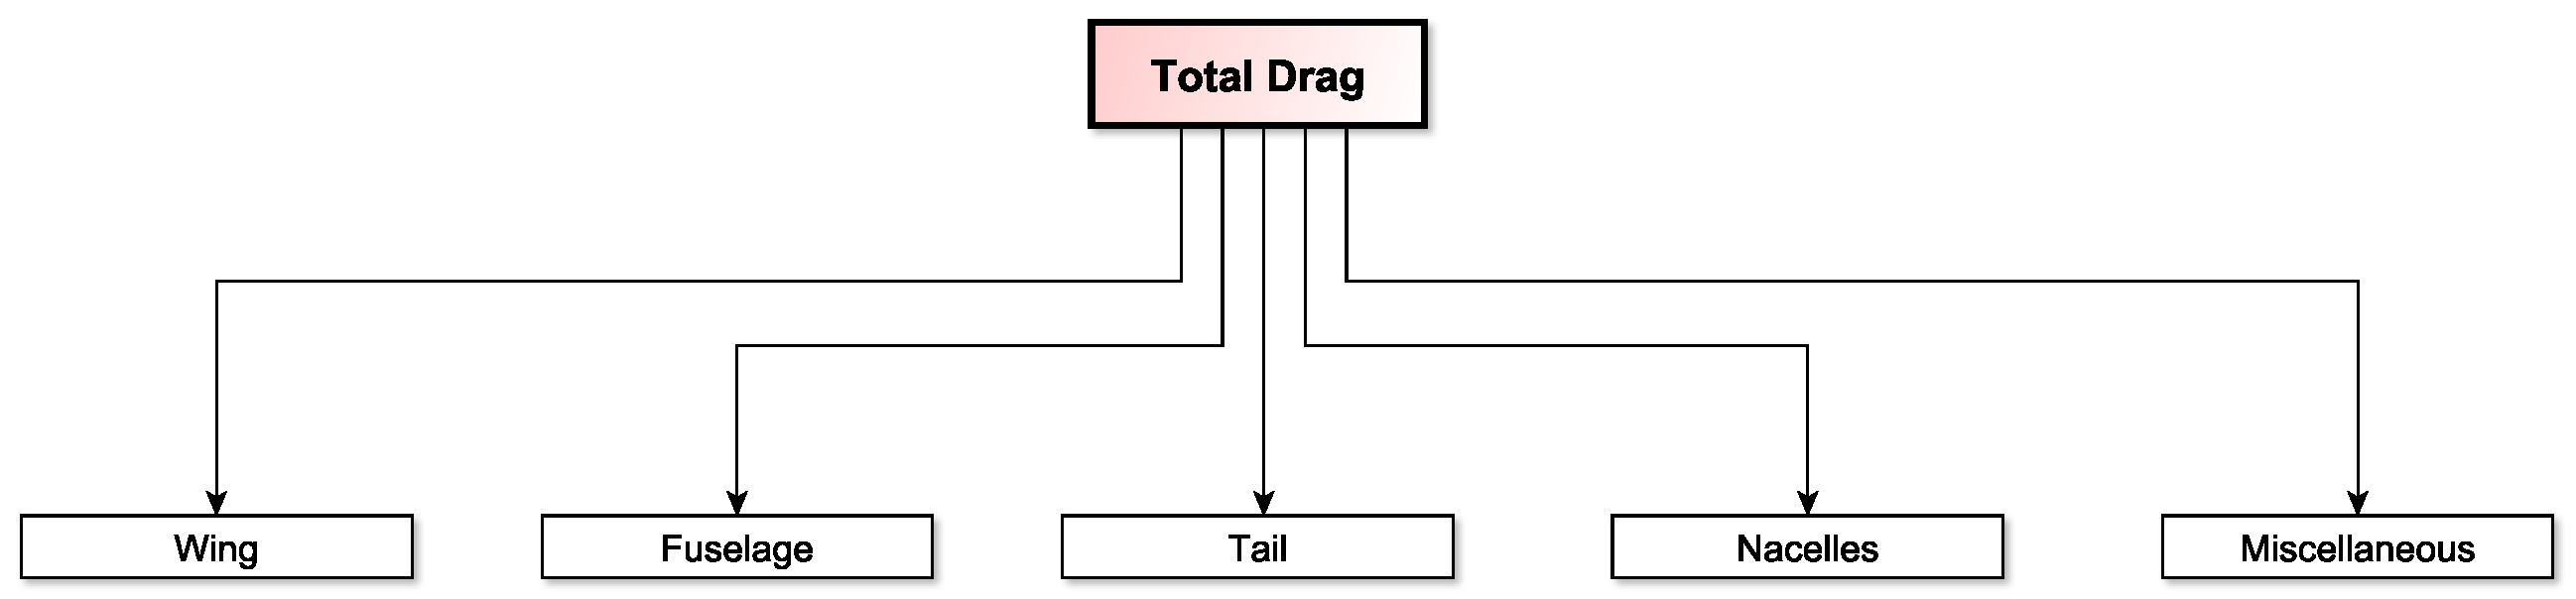
\includegraphics[height=3.6cm]{Immagini/dragco.pdf}} 
\caption{Components breakdown of airplane drags.}
\end{figure}
In JPAD is possible to use different methods in order to evaluate the drag coefficient of a wing and of the entire aircraft. In particular in this section will be explained two approaches and in the next chapter will be shown the results.\\ \\
In order to evaluate the drag coefficient you can divide it into different contributes as shown in the fig. \ref{newcomponent}

\begin{figure}[H]
	\centering
	{\includegraphics[height=6cm]{Immagini/dragfactors.pdf}} 
	\caption{Used breakdown for the wing drag.}
	\label{newcomponent}
\end{figure}

It's possible to evaluate the contributes using different methods.

\subsection{Case 1:  $CD_0$  and $k CL$}
Part of the parasite drag depends on the angle of attack and, consequently, on the CL; while part is constant and it's called $CD_0$. So the contributes of $CD$ which varies with the cl consist of the induced drag (due to vortex) and a part of parasite drag, not considering wave effects. It's possible to approximate the drag polar of a wing as a parabola where the $CD_0$ is the origin. It's important to note that using the parabolic approximation the $CD_0$ is the coefficient drag value at $CL=0$ but this is not properly correct.

\begin{equation}
CD = CD_0 + KCL^2 = CD_0 + \frac{CL^2}{\pi \AR e}
\end{equation}

In order to evaluate the zero lift drag coefficient it's possible to introduce the concept of equivalent parasite area f. This is the area of a thin plate that has the same drag of the wing.

\begin{equation}
f = CD_0 S
\label{cd01}
\end{equation}

Introducing the equivalent friction coefficient, it's possible to express the equivalent parasite area as follows

\begin{equation}
f= S_{wet} C_{f_{e}}
\label{cd02}
\end{equation}

Therefore it is possible to obtain the zero lift drag coefficient by eq. \ref{cd01} and \ref{cd02}.

\begin{equation}
CD_0 =  C_{f_{e}} \left( \frac{S_{wet}}{S}\right)
\end{equation}


\subsection{Case 2: Parasite Drag and Induced Drag}
It's possible to evaluate the parasite drag starting from the airfoils while the contribution that varies with the CL is calculated from the induced angle of attack.

\subsubsection{Parasite Drag}
\begin{enumerate}
	\item First of all the load distribution at a given angle of attack has been calculated
	\item Fifty points along the semispan are defined
	\item For each point, an intermediate profile is calculated
	\item To each profile correspond the lift coefficient at that station
	\item Starting from the CL, using a parabolic approximation for the drag polar, the CD is calculated with the following equation
	\begin{equation}
	CD = CD_{min} + (CL - CL_{CD_{min}})^2 \cdot k
	\end{equation}
	\item Known the drag distribution it is possible to calculate the drag coefficient of the lifting surface integrating
	\end{enumerate}
	
	In the tool it is possible to choose the method used to calculate the load distribution. In particular it's possible to use Shrenk or Nasa-Blackwell method.\\
{\bfseries Schrenk Method} is based on an elliptical lifting coefficient distribution span wise hypothesis on the wing. This method also assumes that the pressure distribution is proportional to the wing area. 
	The {\bfseries Nasa-Blackwell}, as mentioned, is a numerical method for calculating the subsonic load distribution for arbitrary lifting surface arrangements at a fixed angle of attack. \ref{ch:worklift}


\subsubsection{Induced Drag}

The induced drag introduces tridimensional effects on the drag estimation.

\begin{equation}
CD_i = CL \alpha_i
\end{equation}

So it's necessary to evaluate the induced angle of attack along the semi-span(CHAP. \ref{ch:iaoa}).
	
\begin{enumerate}
	\item First of all the load distribution at a given angle of attack has been calculated
	\item At given angle of attack is calculated the distribution of induced angle of attack
	\item Fifty points along the semispan are defined
	\item To each profile correspond the lift coefficient at that station and it's possible to evaluate the local drag coefficien
	\begin{equation}
	Cd =Cl \alpha_i
	\end{equation}
	\item Known the drag distribution it is possible to calculate the drag coefficient of the lifting surface integrating
\end{enumerate}



\section{Java Class Architecture}

In this paragraph the implementation inside the JPAD library of the calculation of the wing drag characteristics will be described. In this library there are several methods relating to the calculation of drag, which are summarized in the table below, all contained in \texttt{LSAerodynamicManager} class. As mentioned the drag may be broken down in different way: using a causal breakdown or a component breakdown, so there are various methods that evaluate the different contributions. In order to have a clear organization of the class, the methods relating to the calculations of the same items are organized in nested classes in  \texttt{LSAerodynamicManager}.\\ 

\begin{table}[H]
\begin{tabular}{p{7cm}p{7.5cm}}
\toprule
\lstinline[language=Java]!calculateCD0Total! & This class contains methods that calculates CD0\\ \hline 
\lstinline[language=Java]!CalcCdWaveDrag! & This method calculates a lifting surface wave drag\\ \hline 
\lstinline[language=Java]!CalcCDAtAlpha! & This method calculates the drag coefficient of the lifting surface using an integral and calling other method that fills the needed field. \\ \hline 
\lstinline[language=Java]!calculateCDParasiteFromAirfoil! &This method calculates drag distribution starting from the load distribution calculated with Nasa-Blackwell method or Schrenk method using a parabolic approximation for the drag polar.  
\\ \hline 
\lstinline[language=Java]!CalculateCdAirfoil! & This nested class has some methods that evaluates the cd of an airfoil corresponding to an alpha that is the input value of the method. The difference between the methods is the way to calculate cl from alpha.\\ \hline 
\lstinline[language=Java]!PlotCDvsAlphaCurve! & This method draws CD vs Alpha curve and CD vs CL curve of a wing, using 30 value of alpha between $\alpha=- 2^{\circ}$ and $\alpha = 18^{\circ}$.\\ \hline 
\lstinline[language=Java]!calculateCDInduced! & This method calculates the cd induced from cl distribution and induced angle of attack. \\ \hline 
\bottomrule
\end{tabular}
\caption{Methods for drag coefficient calculator of a lifting surface.}
\label{table:Table2}
\end{table}

As mentioned it's possible to evaluate the drag coefficient in JPAD using different methods. \\
The first method is to evaluate the zero lift drag coefficient using the nested class \texttt{calculate} \texttt{CD0Total}. In order to evaluate the induced drag it's possible to evaluate the CL of the wing and the oswald factor from an aerodynamic analysis.\\
The second method is to evaluate th CD0 as the zero lift defining an object of the class  \texttt{CalcCDAtAlpha}. This class evaluates the drag coefficient of a lifting surface. This method calls a method of an other class \texttt{CalcCdDistribution} in order to evaluate the Cd distribution at alpha. The drag coefficient distribution is calculated starting from the lift distribution and using a parabolic approximation for the lifting surface polar by the class \texttt{CalculateCd}.  In order to evaluate the induced drag it's necessary to use the method \texttt{calculateCDInduced} that calculate the wing lift distribution using NasaBlackwell method and the induced angle of attack using the methods of the class \texttt{AlphaEffective}.\\
The process are shown in following figures.
\noindent\\
\begin{figure}[H]
\centering
{\includegraphics[height=7cm,  angle=90]{immagini/dragflowchartcd0.pdf}}
\caption{Flow chart of drag estimation classes. Case 1.}
\label{fig:cd}
\end{figure}

\begin{figure}[H]
\centering
{\includegraphics[height=12.9cm, angle=90]{immagini/dragflowchart3.pdf}}
\caption{Flow chart of drag estimation classes. Case 2.}
\label{fig:cd}
\end{figure}




\section{Case Study}

In this section will present the results of the application of the previously introduced method on two aircraft: ATR-72 and B747-100B.
After initializing the Test class and defining the work object, it is possible to define an object of the class \texttt{CalcCDAtAlpha} that calculates the drag coefficient of a wing at a given angle of attack. This method accepts as input three parameters: the angle of attack of the wing,  the method used in order to calculate of lift distribution and an object of the lifting surface aerodynamic manager.
\noindent \\
\begin{lstlisting}[frame=rbl,caption={{\footnotesize Use of Drag Calculator class}},label= [style=\bfseries]{Listing}]

// -----------------------------------------------------------------------
// DRAG CHARACTERISTICS 
// ----------------------------------------------------------------------


System.out.println("\n\n------------------------------------");
System.out.println("\n DRAG CHARACTERISTICS  ");
System.out.println("\n------------------------------------");


         System.out.println("\n ------------------- ");
		System.out.println("|       WING        |");
		System.out.println(" ------------------- \n\n");



		//-----------------------------------------------CDairfoil+ CL*alpha_i


		// parasite Drag

		LSAerodynamicsManager.CalcCdvsAlpha theCDWingArrayCalculator = theLSAnalysis
				.new CalcCdvsAlpha();

		LSAerodynamicsManager.CalcCDAtAlpha theCDWingCalculator = theLSAnalysis
				.new CalcCDAtAlpha();

		parasiteCDWingCleanArray = new double [nValueAlpha];

		Double [] cDWingTemp =  theCDWingArrayCalculator
		.calculateCDParasiteFromAirfoil(alphaMinWing, alphaMaxWing, nValueAlpha);
		
		for (int i=0; i< parasiteCDWingCleanArray.length; i++){
			parasiteCDWingCleanArray[i] =(double)cDWingTemp[i];
		}


		// Induced Drag 

		inducedCDWingArray = theCDWingArrayCalculator
		            .calculateCDInduced(alphaMinWing, alphaMaxWing, nValueAlpha);


		// Total drag

		cDWingCleanArray = new double [nValueAlpha];
		
		for (int i = 0; i<nValueAlpha; i++){
			cDWingCleanArray[i] = parasiteCDWingCleanArray[i]+ 
			   inducedCDWingArray[i];
		}	
}


// Total Drag with Parabolic interpolation

		theWing.calculateFormFactor(theWing.getAerodynamics()
		                       .calculateCompressibility(
		                               theOperatingConditions.get_machCurrent()));
		double cD0WingPolar= theWing.getAerodynamics().calculateCd0Parasite();

		double oswaldFactor = aircraft.get_theAerodynamics().calculateOswald(
				theOperatingConditions.get_machCurrent(), MethodEnum.HOWE);
		System.out.println("oswald factor " + oswaldFactor);

		cD0WingPolarArray = new double [alphaStabilityArray.size()];
		cDiWingPolarArray = new double [alphaStabilityArray.size()];
		cDWaweWingPolarArray = new double [alphaStabilityArray.size()];
		cDWingPolarArray = new double [alphaStabilityArray.size()];


		for (int i=0; i<alphaStabilityArray.size(); i++){

			double cLLocal = theCLWingCalculator.nasaBlackwellAlphaBody(
			 Amount.valueOf(Math.toRadians 
			 (alphaStabilityArray.get(i)), SI.RADIAN));	
			 
			cD0WingPolarArray[i] = cD0WingPolar;
			cDiWingPolarArray[i] = (Math.pow(cLLocal, 2))/
			    (Math.PI * theWing.get_aspectRatio() * oswaldFactor);
			    
			cDWaweWingPolarArray[i] = theWing.getAerodynamics()
			  .getCalculateCdWaveDrag().lockKorn(
			           cLLocal, theOperatingConditions.get_machCurrent());

			cDWingPolarArray[i] = cD0WingPolar + cDiWingPolarArray[i]
			        + cDWaweWingPolarArray[i];
		}
		
		

\end{lstlisting}


%\begin{lstlisting}[caption={{\footnotesize Drag Characteristics of a Lifting Surface - Results. ATR-72}},label= [style=\bfseries]{Listing}]
%------------------------------------
%
% DRAG CHARACTERISTICS  
%
%------------------------------------
%
% ------------------- 
%|       WING        |
% ------------------- 
%
% CD of Wing at alpha body = 2.0 ° is 0.0145499801315
% 
% 
% 	 	 WRITING CHART TO FILE. Parabolic Polar. 
%-----------------------------------------------------
%	 	 DONE 
%	 	 
%\end{lstlisting}

\noindent \\

\subsection{ATR-72}

Following there are the summary diagrams of the results obtained for the ATR 72. In case 2, actually, there are not  contemplated the not linear effects due to induced drag.

\noindent \\ \\
\begin{figure}[H]
\centering
%Parasite Drag coefficient vs CL for WING 
\begin{tikzpicture}

\begin{axis}[
width=16.01cm,
height=10.3cm,
scaled ticks=false,tick label style={/pgf/number format/precision=3},
xmin=0.005,
xmax=0.014,
xtick={0.005,0.006,0.007,0.008,0.009,0.010,0.011,0.012,0.013, 0.014},
xlabel={CD},
xmajorgrids,
ymin=-0.2,
ymax=1.8,
ylabel={CL },
ymajorgrids,
]

\addplot [
color=black,
solid
]
table[row sep=crcr]{
0.007469296190450597	-0.22858740939758343\\
0.007287022428214184	-0.174431561899826\\
0.0071169814112472495	-0.12027571440206852\\
0.0069741242726569334	-0.06611986690431107\\
0.006855731480400362	-0.011964019406553589\\
0.0067522891220144115	0.042191828091203865\\
0.006685549001387827	0.09634767558896132\\
0.006631041182291946	0.15050352308671877\\
0.006606433303131648	0.20465937058447625\\
0.006603728643155777	0.25881521808223373\\
0.006618820348767252	0.31297106557999116\\
0.00666740489582362	0.36712691307774864\\
0.006728192794652587	0.42128276057550607\\
0.006821834279760344	0.47543860807326355\\
0.006934505669583168	0.529594455571021\\
0.007067566243029276	0.5837503030687785\\
0.007231887770792964	0.6379061505665359\\
0.00740844189691754	0.6920619980642934\\
0.0076203349353068705	0.7462178455620508\\
0.007848538349722095	0.8003736930598083\\
0.008099848130174003	0.8545295405575658\\
0.008379701068671232	0.9086853880553232\\
0.00867178678918788	0.9628412355530805\\
0.009001930053764956	1.016997083050838\\
0.009345665298363613	1.0711781714515032\\
0.009715225305003272	1.1262615894992145\\
0.010110645515524467	1.1821772552482097\\
0.010519676359667522	1.2382339475298996\\
0.010965431039632883	1.2937404451756982\\
0.011419260142847611	1.348005527017018\\
0.011890841747483585	1.400337971885271\\
0.01236429783147128	1.4500465586118716\\
0.01283907707735431	1.4964400660282302\\
};
\end{axis}
\end{tikzpicture}%

\caption{ATR 72 CD vs CL at Mach 0.4. Parasite Drag.}
\label{fig:DragATR}
\end{figure}

\begin{figure}[H]
\centering
%Parasite Drag coefficient vs Alpha Wing for WING 
\begin{tikzpicture}

\begin{axis}[
width=14.01 cm,
height=10.3 cm,
scaled ticks=false, tick label style={/pgf/number format/.cd},
xmin=-3,
xmax=21,
xlabel={$\alpha_w$ (deg)},
ytick={0.005,0.007,0.009,0.011,0.013,0.015,0.017},
yticklabels={0.005,0.007,0.009,0.011,0.013,0.015,0.017},
xmajorgrids,
ymin=0.005,
ymax=0.017,
ylabel={$CD_p$},
ymajorgrids,
]

\addplot [
color=black,
solid
]
table[row sep=crcr]{
-3.499999999999999	0.007469296190450597\\
-2.948979591836734	0.007287022428214184\\
-2.3979591836734686	0.0071169814112472495\\
-1.8469387755102034	0.0069741242726569334\\
-1.295918367346938	0.006855731480400362\\
-0.744897959183673	0.0067522891220144115\\
-0.19387755102040782	0.006685549001387827\\
0.3571428571428573	0.006631041182291946\\
0.9081632653061225	0.006606433303131648\\
1.4591836734693877	0.006603728643155777\\
2.010204081632653	0.006618820348767252\\
2.561224489795918	0.00666740489582362\\
3.1122448979591835	0.006728192794652587\\
3.6632653061224487	0.006821834279760344\\
4.2142857142857135	0.006934505669583168\\
4.765306122448979	0.007067566243029276\\
5.316326530612244	0.007231887770792964\\
5.867346938775509	0.00740844189691754\\
6.4183673469387745	0.0076203349353068705\\
6.96938775510204	0.007848538349722095\\
7.520408163265305	0.008099848130174003\\
8.07142857142857	0.008379701068671232\\
8.622448979591834	0.00867178678918788\\
9.173469387755098	0.009001930053764956\\
9.724489795918362	0.009345665298363613\\
10.275510204081627	0.009715225305003272\\
10.826530612244891	0.010110645515524467\\
11.377551020408156	0.010519676359667522\\
11.92857142857142	0.010965431039632883\\
12.479591836734684	0.011419260142847611\\
13.030612244897949	0.011890841747483585\\
13.581632653061213	0.01236429783147128\\
14.132653061224477	0.01283907707735431\\
14.683673469387742	0.013293772809169936\\
15.234693877551006	0.013735560491375176\\
15.78571428571427	0.014136750409501173\\
16.336734693877535	0.014495760714179124\\
16.8877551020408	0.014815403379638891\\
17.438775510204064	0.015042776940536124\\
17.989795918367328	0.015231851626117395\\
18.540816326530592	0.015301700404206387\\
19.091836734693857	0.015300291149208927\\
19.64285714285712	0.015211179699643527\\
20.193877551020385	0.014993068973875793\\
20.74489795918365	0.014722373777723178\\
21.295918367346914	0.014295898758698347\\
21.84693877551018	0.013813931523028981\\
22.397959183673443	0.013241158841941282\\
22.948979591836707	0.012598060285502822\\
23.499999999999993	0.011923315085156497\\
};
\end{axis}
\end{tikzpicture}%

\caption{ATR 72 CD vs $\alpha_w$ at Mach 0.4. Parasite Drag.}
\label{fig:DragATR}
\end{figure}
\noindent \\\\
\begin{figure}[H]
\centering
%Induced Drag coefficient vs Alpha Wing for WING 
\begin{tikzpicture}

\begin{axis}[
width=14.01cm,
height=10.3cm,
scaled ticks=false, tick label style={/pgf/number format/fixed},
xmin=-4,
xmax=24,
xlabel={$\alpha_w$ (deg)},
xmajorgrids,
ymin=0,
ymax=0.14,
ylabel={$CD_i$},
ymajorgrids,
]

\addplot [
color=black,
solid
]
table[row sep=crcr]{
-3.499999999999999	0.0018331633037926422\\
-3.0333333333333323	0.0011712979201843852\\
-2.5666666666666655	6.569692954007069E-4\\
-2.0999999999999988	2.902816495559188E-4\\
-1.6333333333333322	7.131002184608154E-5\\
-1.1666666666666656	9.983356352615397E-8\\
-0.6999999999999991	7.666662225745013E-5\\
-0.2333333333333325	3.009959490613359E-4\\
0.23333333333333406	6.730434844108653E-4\\
0.7000000000000006	0.0011927352670209439\\
1.1666666666666672	0.0018599681341910795\\
1.6333333333333337	0.0026746103158166844\\
2.1000000000000005	0.0036365021828465406\\
2.5666666666666673	0.004745457138582288\\
3.033333333333334	0.006001262639292208\\
3.500000000000001	0.0074036813290432315\\
3.9666666666666677	0.00895245227247044\\
4.4333333333333345	0.010647292268415955\\
4.900000000000001	0.012487897226977691\\
5.366666666666668	0.014473943592499958\\
5.833333333333335	0.016605089795386163\\
6.300000000000002	0.018880977716283304\\
6.766666666666668	0.02130123414713628\\
7.233333333333335	0.023865472234788708\\
7.700000000000002	0.026573292894167086\\
8.166666666666668	0.029424286179571754\\
8.633333333333335	0.03241803260416669\\
9.100000000000001	0.03555410439936239\\
9.566666666666668	0.03883206670737545\\
10.033333333333335	0.042251478701797976\\
10.500000000000002	0.04581189463248246\\
10.966666666666669	0.04951286479241544\\
11.433333333333335	0.053344489717227384\\
11.900000000000002	0.05724737567234397\\
12.366666666666669	0.06118924945372574\\
12.833333333333336	0.06515613233040367\\
13.300000000000002	0.06913467873879656\\
13.76666666666667	0.0731117602597784\\
14.233333333333336	0.07707438495464058\\
14.700000000000003	0.0810090650412595\\
15.16666666666667	0.08490310899902678\\
15.633333333333336	0.0887425567258037\\
16.1	0.09251402603620704\\
16.566666666666666	0.09620462030676719\\
17.03333333333333	0.09980025064775477\\
17.499999999999996	0.10328594840982823\\
17.96666666666666	0.10664819575179695\\
18.433333333333326	0.10987339261107257\\
18.89999999999999	0.11294783938085332\\
19.366666666666656	0.11585772832868885\\
19.83333333333332	0.11858708714475806\\
20.299999999999986	0.12112013730036239\\
20.76666666666665	0.12344247692097834\\
21.233333333333317	0.1255396082791612\\
21.69999999999998	0.12739693918887274\\
22.166666666666647	0.12899978437812165\\
22.63333333333331	0.13033336684246682\\
23.099999999999977	0.13138281918169903\\
23.56666666666664	0.13213318492179044\\
24.033333333333307	0.13256941982398718\\
24.499999999999993	0.13267639318270993\\
};
\end{axis}
\end{tikzpicture}%

\caption{ATR 72 CD vs $\alpha_w$ at Mach 0.4. Induced Drag.}
\label{fig:DragATR}
\end{figure}

\begin{figure}[H]
\centering
%Total Drag coefficient vs Alpha Wing for WING 
\begin{tikzpicture}


\begin{axis}[
width=14.01cm,
height=10.3cm,
scaled ticks=false, tick label style={/pgf/number format/fixed},
xmin=-4,
xmax=24,
xlabel={$\alpha_{w}$ (deg)},
xmajorgrids,
ymin=0,
ymax=0.18,
ylabel={CD},
ymajorgrids,
legend style={at={(0.03,0.85)},anchor=west,draw=black,fill=white,legend cell align=left},
legend entries = {Parasite Drag Coefficient\\Induced Drag Coefficient\\Total Drag Coefficient\\}
]

\addplot [
color=black,
solid
]
table[row sep=crcr]{
-3.499999999999999	0.007469296190450597\\
-2.948979591836734	0.007287022428214184\\
-2.3979591836734686	0.0071169814112472495\\
-1.8469387755102034	0.0069741242726569334\\
-1.295918367346938	0.006855731480400362\\
-0.744897959183673	0.0067522891220144115\\
-0.19387755102040782	0.006685549001387827\\
0.3571428571428573	0.006631041182291946\\
0.9081632653061225	0.006606433303131648\\
1.4591836734693877	0.006603728643155777\\
2.010204081632653	0.006618820348767252\\
2.561224489795918	0.00666740489582362\\
3.1122448979591835	0.006728192794652587\\
3.6632653061224487	0.006821834279760344\\
4.2142857142857135	0.006934505669583168\\
4.765306122448979	0.007067566243029276\\
5.316326530612244	0.007231887770792964\\
5.867346938775509	0.00740844189691754\\
6.4183673469387745	0.0076203349353068705\\
6.96938775510204	0.007848538349722095\\
7.520408163265305	0.008099848130174003\\
8.07142857142857	0.008379701068671232\\
8.622448979591834	0.00867178678918788\\
9.173469387755098	0.009001930053764956\\
9.724489795918362	0.009345665298363613\\
10.275510204081627	0.009715225305003272\\
10.826530612244891	0.010110217470932992\\
11.377551020408156	0.01051859498385748\\
11.92857142857142	0.010944766993420608\\
12.479591836734684	0.0113701068967273\\
13.030612244897949	0.01179159428705097\\
13.581632653061213	0.01220071154512784\\
14.132653061224477	0.012601096945148143\\
14.683673469387742	0.012968323146280034\\
15.234693877551006	0.01332083373358831\\
15.78571428571427	0.013631601036645175\\
16.336734693877535	0.013907471377240542\\
16.8877551020408	0.01415077121953851\\
17.438775510204064	0.01432706370409835\\
17.989795918367328	0.014476671348850757\\
18.540816326530592	0.014546747908528218\\
19.091836734693857	0.014571720687687664\\
19.64285714285712	0.01454118112159416\\
20.193877551020385	0.014430718765284102\\
20.74489795918365	0.014287561000013294\\
21.295918367346914	0.014046319926293457\\
21.84693877551018	0.013767265662881984\\
22.397959183673443	0.013426335270884198\\
22.948979591836707	0.013025155939983924\\
23.499999999999993	0.012596864586577515\\
};

\addplot [
color=black,
densely dashed
]
table[row sep=crcr]{
-3.499999999999999	0.001506728868418428\\
-2.948979591836734	8.718978715119932E-4\\
-2.3979591836734686	4.093875785644783E-4\\
-1.8469387755102034	1.1956488981620044E-4\\
-1.295918367346938	2.662942083053441E-6\\
-0.744897959183673	5.877771159973019E-5\\
-0.19387755102040782	2.878666036114163E-4\\
0.3571428571428573	6.897490774507715E-4\\
0.9081632653061225	0.001264109285404233\\
1.4591836734693877	0.0020105006344846707\\
2.010204081632653	0.002928352116212736\\
2.561224489795918	0.004016976194159838\\
3.1122448979591835	0.00527557799510206\\
3.6632653061224487	0.006703265519046891\\
4.2142857142857135	0.008299060566984793\\
4.765306122448979	0.010061910082839605\\
5.316326530612244	0.011990697616696154\\
5.867346938775509	0.014084254638179423\\
6.4183673469387745	0.0163413714595444\\
6.96938775510204	0.01876080756503307\\
7.520408163265305	0.021341301183717912\\
8.07142857142857	0.02408157798492496\\
8.622448979591834	0.026980358816191978\\
9.173469387755098	0.030036366441850492\\
9.724489795918362	0.03324833127432838\\
10.275510204081627	0.03661499611936733\\
10.826530612244891	0.040135119980031594\\
11.377551020408156	0.04380748098262545\\
11.92857142857142	0.047630878500648344\\
12.479591836734684	0.051604134561135925\\
13.030612244897949	0.05572609462178527\\
13.581632653061213	0.059995627807757045\\
14.132653061224477	0.06441162669475081\\
14.683673469387742	0.06897300672043548\\
15.234693877551006	0.07367870530031043\\
15.78571428571427	0.07852768071700708\\
16.336734693877535	0.08351891084446106\\
16.8877551020408	0.08865139176062913\\
17.438775510204064	0.09392413629477943\\
17.989795918367328	0.09933617254811025\\
18.540816326530592	0.10488654241964265\\
19.091836734693857	0.11057430016315997\\
19.64285714285712	0.11639851099539555\\
20.193877551020385	0.12235824977081347\\
20.74489795918365	0.12845259973409223\\
21.295918367346914	0.13468065135781573\\
21.84693877551018	0.14104150126987108\\
22.397959183673443	0.14753425127255826\\
22.948979591836707	0.15415800745339076\\
23.499999999999993	0.16091187938600324\\
};

\addplot [
color=black,
dashdotted
]
table[row sep=crcr]{
-3.499999999999999	0.008976025058869026\\
-2.948979591836734	0.008158920299726178\\
-2.3979591836734686	0.007526368989811728\\
-1.8469387755102034	0.007093689162473134\\
-1.295918367346938	0.006858394422483416\\
-0.744897959183673	0.006811066833614141\\
-0.19387755102040782	0.006973415604999244\\
0.3571428571428573	0.0073207902597427175\\
0.9081632653061225	0.007870542588535881\\
1.4591836734693877	0.008614229277640446\\
2.010204081632653	0.009547172464979988\\
2.561224489795918	0.010684381089983458\\
3.1122448979591835	0.012003770789754648\\
3.6632653061224487	0.013525099798807234\\
4.2142857142857135	0.01523356623656796\\
4.765306122448979	0.01712947632586888\\
5.316326530612244	0.019222585387489118\\
5.867346938775509	0.021492696535096965\\
6.4183673469387745	0.02396170639485127\\
6.96938775510204	0.026609345914755167\\
7.520408163265305	0.029441149313891916\\
8.07142857142857	0.03246127905359619\\
8.622448979591834	0.03565214560537986\\
9.173469387755098	0.03903829649561545\\
9.724489795918362	0.04259399657269199\\
10.275510204081627	0.046330221424370606\\
10.826530612244891	0.050245337450964586\\
11.377551020408156	0.05432607596648293\\
11.92857142857142	0.05857564549406895\\
12.479591836734684	0.06297424145786322\\
13.030612244897949	0.06751768890883625\\
13.581632653061213	0.07219633935288489\\
14.132653061224477	0.07701272363989896\\
14.683673469387742	0.08194132986671551\\
15.234693877551006	0.08699953903389873\\
15.78571428571427	0.09215928175365226\\
16.336734693877535	0.09742638222170161\\
16.8877551020408	0.10280216298016763\\
17.438775510204064	0.10825119999887778\\
17.989795918367328	0.113812843896961\\
18.540816326530592	0.11943329032817088\\
19.091836734693857	0.12514602085084764\\
19.64285714285712	0.13093969211698972\\
20.193877551020385	0.13678896853609757\\
20.74489795918365	0.14274016073410553\\
21.295918367346914	0.1487269712841092\\
21.84693877551018	0.15480876693275306\\
22.397959183673443	0.16096058654344245\\
22.948979591836707	0.1671831633933747\\
23.499999999999993	0.17350874397258076\\
};
\end{axis}
\end{tikzpicture}%

\caption{ATR 72 CD vs $\alpha_w$\  at Mach 0.4. Drag Coefficients calculated as case 2.}
\label{fig:DragATR}
\end{figure}
\noindent \\
\begin{figure}[H]
\centering
%Drag coefficient contributes vs Alpha Wing for WING 
\begin{tikzpicture}

\begin{axis}[
width=14.01cm,
height=10.3cm,
scaled ticks=false, tick label style={/pgf/number format/fixed},
xmin=-4,
xmax=21,
xlabel={$\alpha_{w}$ (deg)},
xmajorgrids,
ymin=0,
ymax=0.075,
ylabel={CD},
ymajorgrids,
legend style={at={(0.03,0.85)},anchor=west,draw=black,fill=white,legend cell align=left},
legend entries = {$CD_0$\\Induced Drag Coefficient\\Total Drag Coefficient\\}
]

\addplot [
color=black,
solid
]
table[row sep=crcr]{
-3.499999999999999	0.005994554742673666\\
-3.0333333333333323	0.005994554742673666\\
-2.5666666666666655	0.005994554742673666\\
-2.0999999999999988	0.005994554742673666\\
-1.6333333333333322	0.005994554742673666\\
-1.1666666666666656	0.005994554742673666\\
-0.6999999999999991	0.005994554742673666\\
-0.2333333333333325	0.005994554742673666\\
0.23333333333333406	0.005994554742673666\\
0.7000000000000006	0.005994554742673666\\
1.1666666666666672	0.005994554742673666\\
1.6333333333333337	0.005994554742673666\\
2.1000000000000005	0.005994554742673666\\
2.5666666666666673	0.005994554742673666\\
3.033333333333334	0.005994554742673666\\
3.500000000000001	0.005994554742673666\\
3.9666666666666677	0.005994554742673666\\
4.4333333333333345	0.005994554742673666\\
4.900000000000001	0.005994554742673666\\
5.366666666666668	0.005994554742673666\\
5.833333333333335	0.005994554742673666\\
6.300000000000002	0.005994554742673666\\
6.766666666666668	0.005994554742673666\\
7.233333333333335	0.005994554742673666\\
7.700000000000002	0.005994554742673666\\
8.166666666666668	0.005994554742673666\\
8.633333333333335	0.005994554742673666\\
9.100000000000001	0.005994554742673666\\
9.566666666666668	0.005994554742673666\\
10.033333333333335	0.005994554742673666\\
10.500000000000002	0.005994554742673666\\
10.966666666666669	0.005994554742673666\\
11.433333333333335	0.005994554742673666\\
11.900000000000002	0.005994554742673666\\
12.366666666666669	0.005994554742673666\\
12.833333333333336	0.005994554742673666\\
13.300000000000002	0.005994554742673666\\
13.76666666666667	0.005994554742673666\\
14.233333333333336	0.005994554742673666\\
14.700000000000003	0.005994554742673666\\
15.16666666666667	0.005994554742673666\\
15.633333333333336	0.005994554742673666\\
16.1	0.005994554742673666\\
16.566666666666666	0.005994554742673666\\
17.03333333333333	0.005994554742673666\\
17.499999999999996	0.005994554742673666\\
17.96666666666666	0.005994554742673666\\
18.433333333333326	0.005994554742673666\\
18.89999999999999	0.005994554742673666\\
19.366666666666656	0.005994554742673666\\
19.83333333333332	0.005994554742673666\\
20.299999999999986	0.005994554742673666\\
20.76666666666665	0.005994554742673666\\
21.233333333333317	0.005994554742673666\\
21.69999999999998	0.005994554742673666\\
22.166666666666647	0.005994554742673666\\
22.63333333333331	0.005994554742673666\\
23.099999999999977	0.005994554742673666\\
23.56666666666664	0.005994554742673666\\
24.033333333333307	0.005994554742673666\\
24.499999999999993	0.005994554742673666\\
};

\addplot [
color=black,
dashdotted
]
table[row sep=crcr]{
-3.499999999999999	0.0012496715644902392\\
-3.0333333333333323	7.985235955066921E-4\\
-2.5666666666666655	4.479837084480328E-4\\
-2.0999999999999988	1.9805190331426188E-4\\
-1.6333333333333322	4.872818010537974E-5\\
-1.1666666666666656	1.2538821386067516E-8\\
-0.6999999999999991	5.1904979462281005E-5\\
-0.2333333333333325	2.044055020280643E-4\\
0.23333333333333406	4.575141065187364E-4\\
0.7000000000000006	8.112307929342966E-4\\
1.1666666666666672	0.001265555561274745\\
1.6333333333333337	0.0018204884115400823\\
2.1000000000000005	0.0024760293437303084\\
2.5666666666666673	0.003232178357845422\\
3.033333333333334	0.004088935453885423\\
3.500000000000001	0.005046300631850316\\
3.9666666666666677	0.006104273891740096\\
4.4333333333333345	0.007262855233554768\\
4.900000000000001	0.008522044657294323\\
5.366666666666668	0.009881842162958765\\
5.833333333333335	0.011342247750548099\\
6.300000000000002	0.012903261420062323\\
6.766666666666668	0.01456488317150144\\
7.233333333333335	0.016327113004865428\\
7.700000000000002	0.018189950920154324\\
8.166666666666668	0.020153396917368095\\
8.633333333333335	0.02221745099650677\\
9.100000000000001	0.02438211315757031\\
9.566666666666668	0.02664738340055875\\
10.033333333333335	0.029033356637495372\\
10.500000000000002	0.03156267673773693\\
10.966666666666669	0.03421649961023554\\
11.433333333333335	0.036971673386937645\\
11.900000000000002	0.03980119505012025\\
12.366666666666669	0.04267427379438299\\
12.833333333333336	0.04555648156213835\\
13.300000000000002	0.048409990752600544\\
13.76666666666667	0.051193899104271266\\
14.233333333333336	0.05386464175092499\\
14.700000000000003	0.05637649045109086\\
15.16666666666667	0.05868213999103391\\
15.633333333333336	0.060733381761233385\\
16.1	0.06248186450636002\\
16.566666666666666	0.06387994224875072\\
17.03333333333333	0.06488160938538129\\
17.499999999999996	0.0654435229583378\\
17.96666666666666	0.06552611209878559\\
18.433333333333326	0.06509477464443637\\
18.89999999999999	0.06412116093051355\\
19.366666666666656	0.06258454475421564\\
19.83333333333332	0.06047328151267731\\
20.299999999999986	0.05778635351442903\\
20.76666666666665	0.05453500246435518\\
21.233333333333317	0.05074444912214821\\
21.69999999999998	0.0464557001342642\\
22.166666666666647	0.041727442039372786\\
22.63333333333331	0.0366380224473083\\
23.099999999999977	0.031287518391517125\\
23.56666666666664	0.02579989185500342\\
24.033333333333307	0.020325232469773472\\
24.499999999999993	0.015042087389777792\\
};
\addplot [
color=black,
dashed
]
table[row sep=crcr]{
-3.499999999999999	0.007244226307163905\\
-3.0333333333333323	0.006793078338180358\\
-2.5666666666666655	0.006442538451121698\\
-2.0999999999999988	0.006192606645987928\\
-1.6333333333333322	0.0060432829227790455\\
-1.1666666666666656	0.005994567281495051\\
-0.6999999999999991	0.006046459722135947\\
-0.2333333333333325	0.00619896024470173\\
0.23333333333333406	0.006452068849192402\\
0.7000000000000006	0.0068057855356079625\\
1.1666666666666672	0.007260110303948411\\
1.6333333333333337	0.007815043154213748\\
2.1000000000000005	0.008470584086403974\\
2.5666666666666673	0.009226733100519087\\
3.033333333333334	0.010083490196559089\\
3.500000000000001	0.011040855374523982\\
3.9666666666666677	0.012098828634413762\\
4.4333333333333345	0.013257409976228433\\
4.900000000000001	0.014516599399967987\\
5.366666666666668	0.01587639690563243\\
5.833333333333335	0.017336802493221764\\
6.300000000000002	0.01889781616273599\\
6.766666666666668	0.020559437914175107\\
7.233333333333335	0.022321667747539093\\
7.700000000000002	0.02418450566282799\\
8.166666666666668	0.02614795166004176\\
8.633333333333335	0.028212005739180434\\
9.100000000000001	0.030376667900243976\\
9.566666666666668	0.032641938143232414\\
10.033333333333335	0.03502791138016904\\
10.500000000000002	0.0375572314804106\\
10.966666666666669	0.040211054352909205\\
11.433333333333335	0.04296622812961131\\
11.900000000000002	0.04579574979279392\\
12.366666666666669	0.04866882853705665\\
12.833333333333336	0.05155103630481202\\
13.300000000000002	0.05440454549527421\\
13.76666666666667	0.05718845384694493\\
14.233333333333336	0.05985919649359865\\
14.700000000000003	0.062371045193764525\\
15.16666666666667	0.06467669473370757\\
15.633333333333336	0.06672793650390706\\
16.1	0.0684764192490337\\
16.566666666666666	0.0698744969914244\\
17.03333333333333	0.07087616412805496\\
17.499999999999996	0.07143807770101147\\
17.96666666666666	0.07152066684145926\\
18.433333333333326	0.07108932938711005\\
18.89999999999999	0.07011571567318722\\
19.366666666666656	0.06857909949688931\\
19.83333333333332	0.06646783625535098\\
20.299999999999986	0.0637809082571027\\
20.76666666666665	0.06052955720702884\\
21.233333333333317	0.05673900386482188\\
21.69999999999998	0.052450254876937864\\
22.166666666666647	0.04772199678204645\\
22.63333333333331	0.042632577189981966\\
23.099999999999977	0.03728207313419079\\
23.56666666666664	0.031794446597677085\\
24.033333333333307	0.026319787212447137\\
24.499999999999993	0.021036642132451457\\
};
\end{axis}
\end{tikzpicture}%
\caption{ATR 72 CD vs $\alpha_w$  at Mach 0.4. Drag Coefficients calculated as case 1.}
\label{fig:DragATR}
\end{figure}

\begin{figure}[H]
\centering
%Comparison of CD estimation
\begin{tikzpicture}

\begin{axis}[
width=14.01cm,
height=10.3cm,
scaled ticks=false, tick label style={/pgf/number format/fixed},
xmin=-3,
xmax=25,
xlabel={$\alpha_{w}$ (deg)},
xmajorgrids,
ymin=0,
ymax=0.18,
ylabel={CD},
ymajorgrids,
legend style={at={(0.03,0.9)},anchor=west,draw=black,fill=white,legend cell align=left},
legend entries = {Case 2\\Case 1\\}
]

\addplot [
color=black,
solid
]
table[row sep=crcr]{
-3.499999999999999	0.008976025058869026\\
-2.948979591836734	0.008158920299726178\\
-2.3979591836734686	0.007526368989811728\\
-1.8469387755102034	0.007093689162473134\\
-1.295918367346938	0.006858394422483416\\
-0.744897959183673	0.006811066833614141\\
-0.19387755102040782	0.006973415604999244\\
0.3571428571428573	0.0073207902597427175\\
0.9081632653061225	0.007870542588535881\\
1.4591836734693877	0.008614229277640446\\
2.010204081632653	0.009547172464979988\\
2.561224489795918	0.010684381089983458\\
3.1122448979591835	0.012003770789754648\\
3.6632653061224487	0.013525099798807234\\
4.2142857142857135	0.01523356623656796\\
4.765306122448979	0.01712947632586888\\
5.316326530612244	0.019222585387489118\\
5.867346938775509	0.021492696535096965\\
6.4183673469387745	0.02396170639485127\\
6.96938775510204	0.026609345914755167\\
7.520408163265305	0.029441149313891916\\
8.07142857142857	0.03246127905359619\\
8.622448979591834	0.03565214560537986\\
9.173469387755098	0.03903829649561545\\
9.724489795918362	0.04259399657269199\\
10.275510204081627	0.046330221424370606\\
10.826530612244891	0.050245337450964586\\
11.377551020408156	0.05432607596648293\\
11.92857142857142	0.05857564549406895\\
12.479591836734684	0.06297424145786322\\
13.030612244897949	0.06751768890883625\\
13.581632653061213	0.07219633935288489\\
14.132653061224477	0.07701272363989896\\
14.683673469387742	0.08194132986671551\\
15.234693877551006	0.08699953903389873\\
15.78571428571427	0.09215928175365226\\
16.336734693877535	0.09742638222170161\\
16.8877551020408	0.10280216298016763\\
17.438775510204064	0.10825119999887778\\
17.989795918367328	0.113812843896961\\
18.540816326530592	0.11943329032817088\\
19.091836734693857	0.12514602085084764\\
19.64285714285712	0.13093969211698972\\
20.193877551020385	0.13678896853609757\\
20.74489795918365	0.14274016073410553\\
21.295918367346914	0.1487269712841092\\
21.84693877551018	0.15480876693275306\\
22.397959183673443	0.16096058654344245\\
22.948979591836707	0.1671831633933747\\
23.499999999999993	0.17350874397258076\\
};

\addplot [
color=black,
densely dashed
]
table[row sep=crcr]{
-3.499999999999999	0.007430937015312684\\
-2.948979591836734	0.00673414972517081\\
-2.3979591836734686	0.006224624618254807\\
-1.8469387755102034	0.005902361694564677\\
-1.295918367346938	0.005767360954100419\\
-0.744897959183673	0.005819622396862034\\
-0.19387755102040782	0.006059146022849521\\
0.3571428571428573	0.006485931832062881\\
0.9081632653061225	0.0070999798245021135\\
1.4591836734693877	0.007901290000167219\\
2.010204081632653	0.008889862359058195\\
2.561224489795918	0.010065696901175047\\
3.1122448979591835	0.011428793626517768\\
3.6632653061224487	0.012979152535086358\\
4.2142857142857135	0.014716773626880831\\
4.765306122448979	0.016641656901901166\\
5.316326530612244	0.018753802360147374\\
5.867346938775509	0.02105321000161946\\
6.4183673469387745	0.023539879826317417\\
6.96938775510204	0.026213811834241246\\
7.520408163265305	0.029075006025390954\\
8.07142857142857	0.03212346239976653\\
8.622448979591834	0.03535918095736797\\
9.173469387755098	0.03878216169819528\\
9.724489795918362	0.042393496442534775\\
10.275510204081627	0.046227846253873967\\
10.826530612244891	0.05026541976725121\\
11.377551020408156	0.05444794547108174\\
11.92857142857142	0.05870666159993574\\
12.479591836734684	0.0629627904452382\\
13.030612244897949	0.06712838215976859\\
13.581632653061213	0.07110752805595974\\
14.132653061224477	0.0747979433979958\\
14.683673469387742	0.0780929196877096\\
15.234693877551006	0.08088364644427896\\
15.78571428571427	0.08306190247772294\\
16.336734693877535	0.0845231166561966\\
16.8877551020408	0.0851697981670852\\
17.438775510204064	0.0849153362718977\\
17.989795918367328	0.08368816955495958\\
18.540816326530592	0.08143632466590532\\
19.091836734693857	0.07813232455596866\\
19.64285714285712	0.07377846620807389\\
20.193877551020385	0.06841246786072572\\
20.74489795918365	0.062113485725697255\\
21.295918367346914	0.05500850019951959\\
21.84693877551018	0.04727907156876791\\
22.397959183673443	0.039168465209149274\\
22.948979591836707	0.03098914627838805\\
23.499999999999993	0.023130643902911235\\
};
\end{axis}
\end{tikzpicture}%

\caption{ATR 72 CD vs $\alpha_w$  at Mach 0.4. Method comparison.}
\label{fig:DragATR}
\end{figure}

\noindent \\
\begin{figure}[H]
\centering
%Total Drag coefficient vs Alpha Wing for WING 
\begin{tikzpicture}

\begin{axis}[
width=14.01 cm,
height=10.3 cm,
scaled ticks=false, tick label style={/pgf/number format/fixed},
xmin=-3,
xmax=21,
xlabel={alpha_w (deg)},
xmajorgrids,
ymin=0.0,
ymax=0.18,
ylabel={CD },
ymajorgrids,
legend style={at={(0.03,0.85)},anchor=west,draw=black,fill=white,legend cell align=left},
legend entries = {Clean\\$\delta_{f_1} = 22^{\circ}$ $\delta_{f_2} = 22^{\circ}$ \\$\delta_{f_1} = 30^{\circ}$ $\delta_{f_2} = 30^{\circ}$\\}
]

\addplot [
color=black,
solid
]
table[row sep=crcr]{
-3.499999999999999	0.009081003009475277\\
-3.0333333333333323	0.008338993103897711\\
-2.5666666666666655	0.007731591620866627\\
-2.0999999999999988	0.007286653284181767\\
-1.6333333333333322	0.006978522672743853\\
-1.1666666666666656	0.006830892455597397\\
-0.6999999999999991	0.006822175256027749\\
-0.2333333333333325	0.00697190532354176\\
0.23333333333333406	0.007262559777467914\\
0.7000000000000006	0.007709506765969541\\
1.1666666666666672	0.008299293698377954\\
1.6333333333333337	0.009043131424582317\\
2.1000000000000005	0.009931635491497962\\
2.5666666666666673	0.01097185714164552\\
3.033333333333334	0.012158483821422829\\
3.500000000000001	0.013494411219071002\\
3.9666666666666677	0.014978401592188818\\
4.4333333333333345	0.01660919998210714\\
4.900000000000001	0.01838964730745799\\
5.366666666666668	0.02031433773901089\\
5.833333333333335	0.022390194350623546\\
6.300000000000002	0.024607668740686824\\
6.766666666666668	0.02697777076070086\\
7.233333333333335	0.029486811883411332\\
7.700000000000002	0.03214989298205895\\
8.166666666666668	0.034949189605857224\\
8.633333333333335	0.03790389767480816\\
9.100000000000001	0.04099206096878824\\
9.566666666666668	0.044236974325131656\\
10.033333333333335	0.04761255347089985\\
10.500000000000002	0.051146195704825564\\
10.966666666666669	0.05480872065645977\\
11.433333333333335	0.058628545449192083\\
11.900000000000002	0.06257751096106352\\
12.366666666666669	0.0666671769329739\\
12.833333333333336	0.07083003040344289\\
13.300000000000002	0.07502244332587577\\
13.76666666666667	0.0792378693907562\\
14.233333333333336	0.08345046669961328\\
14.700000000000003	0.08765990992433831\\
15.16666666666667	0.09183983584298142\\
15.633333333333336	0.09598994744537866\\
16.1	0.10008580526553741\\
16.566666666666666	0.10412455833239855\\
17.03333333333333	0.1080849808594734\\
17.499999999999996	0.11196056332880679\\
17.96666666666666	0.11573600989080841\\
18.433333333333326	0.11939667901571477\\
18.89999999999999	0.12293440019864041\\
19.366666666666656	0.1263288583378069\\
19.83333333333332	0.12958002828149182\\
20.299999999999986	0.13265965818304437\\
20.76666666666665	0.13557540217443037\\
21.233333333333317	0.13828846930452418\\
21.69999999999998	0.1408147937762651\\
22.166666666666647	0.14311017779488228\\
22.63333333333331	0.14519828880742952\\
23.099999999999977	0.14702837340871622\\
23.56666666666664	0.1486302458262006\\
24.033333333333307	0.14994823457139508\\
24.499999999999993	0.15101638195133255\\
};

\addplot [
color=black,
densely dashed
]
table[row sep=crcr]{
-3.499999999999999	0.028648344942790366\\
-3.0333333333333323	0.0279063350372128\\
-2.5666666666666655	0.027298933554181712\\
-2.0999999999999988	0.026853995217496852\\
-1.6333333333333322	0.02654586460605894\\
-1.1666666666666656	0.026398234388912485\\
-0.6999999999999991	0.026389517189342834\\
-0.2333333333333325	0.026539247256856847\\
0.23333333333333406	0.026829901710783\\
0.7000000000000006	0.02727684869928463\\
1.1666666666666672	0.02786663563169304\\
1.6333333333333337	0.028610473357897404\\
2.1000000000000005	0.02949897742481305\\
2.5666666666666673	0.030539199074960607\\
3.033333333333334	0.03172582575473792\\
3.500000000000001	0.03306175315238609\\
3.9666666666666677	0.03454574352550391\\
4.4333333333333345	0.03617654191542223\\
4.900000000000001	0.03795698924077308\\
5.366666666666668	0.039881679672325976\\
5.833333333333335	0.04195753628393863\\
6.300000000000002	0.04417501067400191\\
6.766666666666668	0.04654511269401595\\
7.233333333333335	0.04905415381672642\\
7.700000000000002	0.051717234915374034\\
8.166666666666668	0.05451653153917231\\
8.633333333333335	0.05747123960812325\\
9.100000000000001	0.06055940290210333\\
9.566666666666668	0.06380431625844674\\
10.033333333333335	0.06717989540421493\\
10.500000000000002	0.07071353763814064\\
10.966666666666669	0.07437606258977486\\
11.433333333333335	0.07819588738250717\\
11.900000000000002	0.08214485289437862\\
12.366666666666669	0.086234518866289\\
12.833333333333336	0.09039737233675799\\
13.300000000000002	0.09458978525919085\\
13.76666666666667	0.09880521132407127\\
14.233333333333336	0.10301780863292836\\
14.700000000000003	0.10722725185765339\\
15.16666666666667	0.1114071777762965\\
15.633333333333336	0.11555728937869375\\
16.1	0.1196531471988525\\
16.566666666666666	0.12369190026571364\\
17.03333333333333	0.1276523227927885\\
17.499999999999996	0.13152790526212188\\
17.96666666666666	0.1353033518241235\\
18.433333333333326	0.13896402094902985\\
18.89999999999999	0.1425017421319555\\
19.366666666666656	0.145896200271122\\
19.83333333333332	0.1491473702148069\\
20.299999999999986	0.15222700011635945\\
20.76666666666665	0.15514274410774545\\
21.233333333333317	0.15785581123783926\\
21.69999999999998	0.16038213570958018\\
22.166666666666647	0.16267751972819736\\
22.63333333333331	0.1647656307407446\\
23.099999999999977	0.1665957153420313\\
23.56666666666664	0.16819758775951568\\
24.033333333333307	0.16951557650471016\\
24.499999999999993	0.17058372388464763\\
};
\addplot [
color=black,
dashdotted
]
table[row sep=crcr]{
-3.499999999999999	0.038391566394672165\\
-3.0333333333333323	0.0376495564890946\\
-2.5666666666666655	0.03704215500606351\\
-2.0999999999999988	0.03659721666937865\\
-1.6333333333333322	0.03628908605794074\\
-1.1666666666666656	0.036141455840794284\\
-0.6999999999999991	0.03613273864122463\\
-0.2333333333333325	0.03628246870873865\\
0.23333333333333406	0.0365731231626648\\
0.7000000000000006	0.03702007015116643\\
1.1666666666666672	0.03760985708357484\\
1.6333333333333337	0.0383536948097792\\
2.1000000000000005	0.03924219887669485\\
2.5666666666666673	0.0402824205268424\\
3.033333333333334	0.041469047206619716\\
3.500000000000001	0.04280497460426789\\
3.9666666666666677	0.0442889649773857\\
4.4333333333333345	0.04591976336730402\\
4.900000000000001	0.04770021069265488\\
5.366666666666668	0.049624901124207775\\
5.833333333333335	0.05170075773582043\\
6.300000000000002	0.05391823212588371\\
6.766666666666668	0.05628833414589775\\
7.233333333333335	0.05879737526860822\\
7.700000000000002	0.061460456367255833\\
8.166666666666668	0.0642597529910541\\
8.633333333333335	0.06721446106000505\\
9.100000000000001	0.07030262435398513\\
9.566666666666668	0.07354753771032854\\
10.033333333333335	0.07692311685609673\\
10.500000000000002	0.08045675909002245\\
10.966666666666669	0.08411928404165665\\
11.433333333333335	0.08793910883438896\\
11.900000000000002	0.09188807434626041\\
12.366666666666669	0.09597774031817079\\
12.833333333333336	0.10014059378863978\\
13.300000000000002	0.10433300671107265\\
13.76666666666667	0.10854843277595308\\
14.233333333333336	0.11276103008481017\\
14.700000000000003	0.1169704733095352\\
15.16666666666667	0.1211503992281783\\
15.633333333333336	0.12530051083057553\\
16.1	0.12939636865073428\\
16.566666666666666	0.13343512171759542\\
17.03333333333333	0.1373955442446703\\
17.499999999999996	0.14127112671400366\\
17.96666666666666	0.1450465732760053\\
18.433333333333326	0.14870724240091165\\
18.89999999999999	0.1522449635838373\\
19.366666666666656	0.1556394217230038\\
19.83333333333332	0.1588905916666887\\
20.299999999999986	0.16197022156824126\\
20.76666666666665	0.16488596555962726\\
21.233333333333317	0.16759903268972107\\
21.69999999999998	0.170125357161462\\
22.166666666666647	0.17242074118007916\\
22.63333333333331	0.1745088521926264\\
23.099999999999977	0.1763389367939131\\
23.56666666666664	0.1779408092113975\\
24.033333333333307	0.17925879795659197\\
24.499999999999993	0.18032694533652943\\
};
\end{axis}
\end{tikzpicture}%

\caption{ATR 72 CD vs $\alpha_w$  at Mach 0.2. Clean and Flapped wing.}
\label{fig:DragATR}
\end{figure}


\subsection{BOEING 747-100B}

\begin{figure}[H]
\centering
%Parasite Drag coefficient vs CL for WING 
\begin{tikzpicture}

\begin{axis}[
width=14.01cm,
height=9.3cm,
scaled ticks=false,tick label style={/pgf/number format/precision=3},
xmin=0.0,
xmax=0.021,
xtick={0, 0.003, 0.006,0.009,0.012,0.015,0.018 ,0.021},
xticklabels={0, 0.003, 0.006,0.009,0.012,0.015,0.018 ,0.021},
xlabel={$CD_p$},
xmajorgrids,
ymin=-0.15,
ymax=1.6,
ylabel={CL },
ymajorgrids,
]

\addplot [
color=black,
solid
]
table[row sep=crcr]{
0.005153079224038589	-0.16473803066706622\\
0.005096446795372702	-0.12249674239545955\\
0.0050398143667068135	-0.08025545412385285\\
0.005021170727495726	-0.03801416585224615\\
0.005005341072688699	0.004227122419360546\\
0.005024686043248059	0.046468410690967216\\
0.005049658953866043	0.0887096989625739\\
0.005106992332391768	0.13095098723418058\\
0.005172767572110818	0.17319227550578725\\
0.0052680891071571765	0.21543356377739392\\
0.005374666373756796	0.25767485204900065\\
0.005507976543710377	0.2999161403206073\\
0.005655356662797624	0.342157428592214\\
0.005826655234193474	0.38439871686382066\\
0.006014837418983632	0.4266400051354274\\
0.006224124284159255	0.468881293407034\\
0.00645310885102798	0.5111225816786407\\
0.006700384140897438	0.5533638699502474\\
0.006970171089844721	0.595605158221854\\
0.007255434804408012	0.6378464464934608\\
0.007566024135433859	0.6800877347650675\\
0.007889276274690984	0.7223290230366741\\
0.008240667987795396	0.7645703113082808\\
0.008601908834618838	0.8068115995798874\\
0.008994104101702087	0.849052887851494\\
0.009393728433138208	0.8912941761231006\\
0.009829012273468118	0.9335354643947072\\
0.010268984778003273	0.9758240350364609\\
0.010749592372317224	1.0182939665589794\\
0.011231519924154016	1.0606201988823274\\
0.011750406286630346	1.1024157591875257\\
0.012269292649106676	1.143293674655598\\
0.012811007062792092	1.1828669724675651\\
0.01335353676402069	1.2207486798044505\\
0.013899261245298115	1.2565518238472757\\
0.014445354355042713	1.289889431777063\\
0.014973762145327918	1.320374530774835\\
0.015498485494059081	1.3476201480216132\\
0.015985450532506638	1.3712393106984209\\
0.016460401563136686	1.390845045986279\\
0.01688021454570236	1.406050381066211\\
0.01727521540663907	1.4164683431192384\\
0.017601930038407376	1.4217119593263834\\
0.01788691419679499	1.4213942568686693\\
0.018095967254518428	1.4151282629271167\\
0.01824332629295222	1.402527004682749\\
0.018313702480489247	1.3832035093165875\\
0.018301597042065458	1.3567708040096558\\
0.018218243127443825	1.3228419159429747\\
};
\end{axis}
\end{tikzpicture}%

\caption{BOEING 747-100B CD vs CL at Mach 0.75. Parasite Drag.}
\label{fig:DragATR}
\end{figure}

\begin{figure}[H]
\centering
%Parasite Drag coefficient vs Alpha Wing for WING 
\begin{tikzpicture}

\begin{axis}[
width=14.01 cm,
height=10.3 cm,
scaled ticks=false, tick label style={/pgf/number format/.cd},
xmin=-3,
xmax=23,
xlabel={$\alpha_w$ (deg)},
ytick={0.002, 0.003, 0.004,0.005,0.007,0.009,0.011,0.013,0.015,0.017, 0.019},
yticklabels={0.002, 0.003, 0.004,0.005,0.007,0.009,0.011,0.013,0.015,0.017, 0.019},
xmajorgrids,
ymin=0.005,
ymax=0.019,
ylabel={$CD_p$},
ymajorgrids,
]

\addplot [
color=black,
solid
]
table[row sep=crcr]{
-3.499999999999999	0.005153079224038589\\
-2.999999999999999	0.005096446795372702\\
-2.499999999999999	0.0050398143667068135\\
-1.9999999999999991	0.005021170727495726\\
-1.4999999999999991	0.005005341072688699\\
-0.9999999999999992	0.005024686043248059\\
-0.49999999999999933	0.005049658953866043\\
5.551115123125783E-16	0.005106992332391768\\
0.5000000000000004	0.005172767572110818\\
1.0000000000000004	0.0052680891071571765\\
1.5000000000000004	0.005374666373756796\\
2.0000000000000004	0.005507976543710377\\
2.5000000000000004	0.005655356662797624\\
3.0000000000000004	0.005826655234193474\\
3.5000000000000004	0.006014837418983632\\
4.0	0.006224124284159255\\
4.5	0.00645310885102798\\
5.0	0.006700384140897438\\
5.5	0.006970171089844721\\
6.0	0.007255434804408012\\
6.5	0.007566024135433859\\
7.0	0.007889276274690984\\
7.5	0.008240667987795396\\
8.0	0.008601908834618838\\
8.5	0.008994104101702087\\
9.0	0.009393728433138208\\
9.5	0.009829012273468118\\
10.0	0.010268984778003273\\
10.5	0.010749592372317224\\
11.0	0.011231519924154016\\
11.5	0.011750406286630346\\
12.0	0.012269292649106676\\
12.5	0.012811007062792092\\
13.0	0.01335353676402069\\
13.5	0.013899261245298115\\
14.0	0.014445354355042713\\
14.5	0.014973762145327918\\
15.0	0.015498485494059081\\
15.5	0.015985450532506638\\
16.0	0.016460401563136686\\
16.5	0.01688021454570236\\
17.0	0.01727521540663907\\
17.5	0.017601930038407376\\
18.0	0.01788691419679499\\
18.5	0.018095967254518428\\
19.0	0.01824332629295222\\
19.5	0.018313702480489247\\
20.0	0.018301597042065458\\
20.5	0.018218243127443825\\
21.0	0.018033953871541906\\
21.5	0.017790255658101044\\
22.0	0.01743368042533619\\
22.5	0.01703417002488941\\
23.0	0.016521954809277577\\
23.5	0.015985393093868958\\
24.0	0.015355503129239324\\
24.5	0.014718250033878262\\
25.0	0.014034977371445765\\
25.5	0.013354647767120571\\
26.0	0.012714049447243974\\
26.499999999999993	0.012073451127367388\\
};
\end{axis}
\end{tikzpicture}%

\caption{BOEING 747-100B CD vs $\alpha_w$ at Mach 0.75. Parasite Drag.}
\label{fig:DragATR}
\end{figure}
\noindent \\\\
\begin{figure}[H]
\centering
%Induced Drag coefficient vs Alpha Wing for WING 
\begin{tikzpicture}

\begin{axis}[
width=14.01cm,
height=10.3cm,
scaled ticks=false, tick label style={/pgf/number format/fixed},
xmin=-3,
xmax=25,
xlabel={$\alpha_w$ (deg)},
xmajorgrids,
ymin=0,
ymax=0.15,
ylabel={$CD_i$},
ymajorgrids,
]

\addplot [
color=black,
solid
]
table[row sep=crcr]{
-3.499999999999999	0.0012384974738516574\\
-2.999999999999999	6.704425975451128E-4\\
-2.499999999999999	2.781304454838692E-4\\
-1.9999999999999991	6.177441448148735E-5\\
-1.4999999999999991	2.1465331324102298E-5\\
-0.9999999999999992	1.5722885721536933E-4\\
-0.49999999999999933	4.6890816515685285E-4\\
5.551115123125783E-16	9.562827739330133E-4\\
0.5000000000000004	0.0016190131353428176\\
1.0000000000000004	0.0024566568659538553\\
1.5000000000000004	0.0034686745276853725\\
2.0000000000000004	0.004654436474797163\\
2.5000000000000004	0.006013230558038131\\
3.0000000000000004	0.007544270462077481\\
3.5000000000000004	0.0092467044485457\\
4.0	0.011119624283267284\\
4.5	0.01316207414118553\\
5.0	0.015373059304262242\\
5.5	0.017751554494266825\\
6.0	0.02029651171182452\\
6.5	0.02300686748347157\\
7.0	0.02588154944814377\\
7.5	0.028919482242190226\\
8.0	0.03211959266672412\\
8.5	0.03548081414229564\\
9.0	0.039002202110194395\\
9.5	0.04268735285842411\\
10.0	0.04654001343025939\\
10.5	0.05055884971004246\\
11.0	0.0547384786381617\\
11.5	0.059070896055468905\\
12.0	0.06354356031674095\\
12.5	0.06814127796605951\\
13.0	0.07284892316261692\\
13.5	0.07764698020018104\\
14.0	0.08251228463460303\\
14.5	0.08741930133597117\\
15.0	0.09234015339406235\\
15.5	0.09724464115634104\\
16.0	0.1021002641174278\\
16.5	0.10687236044950474\\
17.0	0.11152428981833395\\
17.5	0.11601673167908687\\
18.0	0.12030809745868151\\
18.5	0.1243545912940463\\
19.0	0.1281101804727538\\
19.5	0.13152716050998597\\
20.0	0.13455595420579292\\
20.5	0.13714497379609109\\
21.0	0.13924063538612172\\
21.5	0.1407873732398225\\
22.0	0.14172765394064685\\
22.5	0.14200199043801315\\
23.0	0.14154895599225853\\
23.5	0.1403051980296759\\
24.0	0.1382054519179844\\
24.5	0.13518255467141582\\
25.0	0.13116745859348466\\
25.5	0.12608924486452538\\
26.0	0.11987513708011498\\
26.499999999999993	0.11245051474565648\\
};
\end{axis}
\end{tikzpicture}%

\caption{BOEING 747-100B CD vs $\alpha_w$ at Mach 0.75. Induced Drag.}
\label{fig:DragATR}
\end{figure}

\begin{figure}[H]
\centering
%Total Drag coefficient vs Alpha Wing for WING 
\begin{tikzpicture}


\begin{axis}[
width=14.01cm,
height=10.3cm,
scaled ticks=false, tick label style={/pgf/number format/fixed},
xmin=-3,
xmax=25,
xlabel={$\alpha_{w}$ (deg)},
xmajorgrids,
ymin=0,
ymax=0.17,
ylabel={CD},
ymajorgrids,
legend style={at={(0.03,0.85)},anchor=west,draw=black,fill=white,legend cell align=left},
legend entries = {Parasite Drag Coefficient\\Induced Drag Coefficient\\Total Drag Coefficient\\}
]

\addplot [
color=black,
solid
]
table[row sep=crcr]{
-3.499999999999999	0.005153079224038589\\
-2.999999999999999	0.005096446795372702\\
-2.499999999999999	0.0050398143667068135\\
-1.9999999999999991	0.005021170727495726\\
-1.4999999999999991	0.005005341072688699\\
-0.9999999999999992	0.005024686043248059\\
-0.49999999999999933	0.005049658953866043\\
5.551115123125783E-16	0.005106992332391768\\
0.5000000000000004	0.005172767572110818\\
1.0000000000000004	0.0052680891071571765\\
1.5000000000000004	0.005374666373756796\\
2.0000000000000004	0.005507976543710377\\
2.5000000000000004	0.005655356662797624\\
3.0000000000000004	0.005826655234193474\\
3.5000000000000004	0.006014837418983632\\
4.0	0.006224124284159255\\
4.5	0.00645310885102798\\
5.0	0.006700384140897438\\
5.5	0.006970171089844721\\
6.0	0.007255434804408012\\
6.5	0.007566024135433859\\
7.0	0.007889276274690984\\
7.5	0.008240667987795396\\
8.0	0.008601908834618838\\
8.5	0.008994104101702087\\
9.0	0.009393728433138208\\
9.5	0.009829012273468118\\
10.0	0.010268984778003273\\
10.5	0.010749592372317224\\
11.0	0.011231519924154016\\
11.5	0.011750406286630346\\
12.0	0.012269292649106676\\
12.5	0.012811007062792092\\
13.0	0.01335353676402069\\
13.5	0.013899261245298115\\
14.0	0.014445354355042713\\
14.5	0.014973762145327918\\
15.0	0.015498485494059081\\
15.5	0.015985450532506638\\
16.0	0.016460401563136686\\
16.5	0.01688021454570236\\
17.0	0.01727521540663907\\
17.5	0.017601930038407376\\
18.0	0.01788691419679499\\
18.5	0.018095967254518428\\
19.0	0.01824332629295222\\
19.5	0.018313702480489247\\
20.0	0.018301597042065458\\
20.5	0.018218243127443825\\
21.0	0.018033953871541906\\
21.5	0.017790255658101044\\
22.0	0.01743368042533619\\
22.5	0.01703417002488941\\
23.0	0.016521954809277577\\
23.5	0.015985393093868958\\
24.0	0.015355503129239324\\
24.5	0.014718250033878262\\
25.0	0.014034977371445765\\
25.5	0.013354647767120571\\
26.0	0.012714049447243974\\
26.499999999999993	0.012073451127367388\\
};

\addplot [
color=black,
densely dashed
]
table[row sep=crcr]{
-3.499999999999999	0.0012384974738516574\\
-2.999999999999999	6.704425975451128E-4\\
-2.499999999999999	2.781304454838692E-4\\
-1.9999999999999991	6.177441448148735E-5\\
-1.4999999999999991	2.1465331324102298E-5\\
-0.9999999999999992	1.5722885721536933E-4\\
-0.49999999999999933	4.6890816515685285E-4\\
5.551115123125783E-16	9.562827739330133E-4\\
0.5000000000000004	0.0016190131353428176\\
1.0000000000000004	0.0024566568659538553\\
1.5000000000000004	0.0034686745276853725\\
2.0000000000000004	0.004654436474797163\\
2.5000000000000004	0.006013230558038131\\
3.0000000000000004	0.007544270462077481\\
3.5000000000000004	0.0092467044485457\\
4.0	0.011119624283267284\\
4.5	0.01316207414118553\\
5.0	0.015373059304262242\\
5.5	0.017751554494266825\\
6.0	0.02029651171182452\\
6.5	0.02300686748347157\\
7.0	0.02588154944814377\\
7.5	0.028919482242190226\\
8.0	0.03211959266672412\\
8.5	0.03548081414229564\\
9.0	0.039002202110194395\\
9.5	0.04268735285842411\\
10.0	0.04654001343025939\\
10.5	0.05055884971004246\\
11.0	0.0547384786381617\\
11.5	0.059070896055468905\\
12.0	0.06354356031674095\\
12.5	0.06814127796605951\\
13.0	0.07284892316261692\\
13.5	0.07764698020018104\\
14.0	0.08251228463460303\\
14.5	0.08741930133597117\\
15.0	0.09234015339406235\\
15.5	0.09724464115634104\\
16.0	0.1021002641174278\\
16.5	0.10687236044950474\\
17.0	0.11152428981833395\\
17.5	0.11601673167908687\\
18.0	0.12030809745868151\\
18.5	0.1243545912940463\\
19.0	0.1281101804727538\\
19.5	0.13152716050998597\\
20.0	0.13455595420579292\\
20.5	0.13714497379609109\\
21.0	0.13924063538612172\\
21.5	0.1407873732398225\\
22.0	0.14172765394064685\\
22.5	0.14200199043801315\\
23.0	0.14154895599225853\\
23.5	0.1403051980296759\\
24.0	0.1382054519179844\\
24.5	0.13518255467141582\\
25.0	0.13116745859348466\\
25.5	0.12608924486452538\\
26.0	0.11987513708011498\\
26.499999999999993	0.11245051474565648\\
};

\addplot [
color=black,
dashdotted
]
table[row sep=crcr]{
-3.499999999999999	0.006391576697890247\\
-2.999999999999999	0.0057668893929178145\\
-2.499999999999999	0.0053179448121906826\\
-1.9999999999999991	0.005082945141977213\\
-1.4999999999999991	0.0050268064040128015\\
-0.9999999999999992	0.005181914900463429\\
-0.49999999999999933	0.005518567119022896\\
5.551115123125783E-16	0.006063275106324781\\
0.5000000000000004	0.0067917807074536355\\
1.0000000000000004	0.007724745973111032\\
1.5000000000000004	0.008843340901442169\\
2.0000000000000004	0.010162413018507541\\
2.5000000000000004	0.011668587220835755\\
3.0000000000000004	0.013370925696270955\\
3.5000000000000004	0.015261541867529333\\
4.0	0.01734374856742654\\
4.5	0.019615182992213508\\
5.0	0.022073443445159678\\
5.5	0.024721725584111544\\
6.0	0.02755194651623253\\
6.5	0.030572891618905428\\
7.0	0.033770825722834755\\
7.5	0.037160150229985624\\
8.0	0.04072150150134296\\
8.5	0.04447491824399773\\
9.0	0.048395930543332605\\
9.5	0.05251636513189223\\
10.0	0.056808998208262663\\
10.5	0.06130844208235968\\
11.0	0.06596999856231571\\
11.5	0.07082130234209925\\
12.0	0.07581285296584762\\
12.5	0.0809522850288516\\
13.0	0.08620245992663761\\
13.5	0.09154624144547915\\
14.0	0.09695763898964574\\
14.5	0.10239306348129909\\
15.0	0.10783863888812142\\
15.5	0.11323009168884768\\
16.0	0.11856066568056449\\
16.5	0.1237525749952071\\
17.0	0.12879950522497302\\
17.5	0.13361866171749426\\
18.0	0.1381950116554765\\
18.5	0.14245055854856473\\
19.0	0.14635350676570602\\
19.5	0.14984086299047522\\
20.0	0.15285755124785838\\
20.5	0.1553632169235349\\
21.0	0.15727458925766363\\
21.5	0.15857762889792354\\
22.0	0.15916133436598304\\
22.5	0.15903616046290256\\
23.0	0.1580709108015361\\
23.5	0.15629059112354485\\
24.0	0.15356095504722372\\
24.5	0.14990080470529407\\
25.0	0.14520243596493043\\
25.5	0.13944389263164594\\
26.0	0.13258918652735896\\
26.499999999999993	0.12452396587302388\\
};
\end{axis}
\end{tikzpicture}%
\caption{BOEING 747-100B CD vs $\alpha_w$\  at Mach 0.75. Drag Coefficients calculated as case 2.}
\label{fig:DragATR}
\end{figure}
\noindent \\\\
\begin{figure}[H]
\centering
%Drag coefficient contributes vs Alpha Wing for WING 
\begin{tikzpicture}

\begin{axis}[
width=14.01cm,
height=10.3cm,
scaled ticks=false, tick label style={/pgf/number format/fixed},
xmin=-3,
xmax=25,
xlabel={$\alpha_{w}$ (deg)},
xmajorgrids,
ymin=0,
ymax=0.11,
ylabel={CD},
ymajorgrids,
legend style={at={(0.03,0.85)},anchor=west,draw=black,fill=white,legend cell align=left},
legend entries = {$CD_0$\\Induced Drag Coefficient\\Total Drag Coefficient\\}
]

\addplot [
color=black,
solid
]
table[row sep=crcr]{
-3.499999999999999	0.004146080035486615\\
-2.999999999999999	0.004146080035486615\\
-2.499999999999999	0.004146080035486615\\
-1.9999999999999991	0.004146080035486615\\
-1.4999999999999991	0.004146080035486615\\
-0.9999999999999992	0.004146080035486615\\
-0.49999999999999933	0.004146080035486615\\
5.551115123125783E-16	0.004146080035486615\\
0.5000000000000004	0.004146080035486615\\
1.0000000000000004	0.004146080035486615\\
1.5000000000000004	0.004146080035486615\\
2.0000000000000004	0.004146080035486615\\
2.5000000000000004	0.004146080035486615\\
3.0000000000000004	0.004146080035486615\\
3.5000000000000004	0.004146080035486615\\
4.0	0.004146080035486615\\
4.5	0.004146080035486615\\
5.0	0.004146080035486615\\
5.5	0.004146080035486615\\
6.0	0.004146080035486615\\
6.5	0.004146080035486615\\
7.0	0.004146080035486615\\
7.5	0.004146080035486615\\
8.0	0.004146080035486615\\
8.5	0.004146080035486615\\
9.0	0.004146080035486615\\
9.5	0.004146080035486615\\
10.0	0.004146080035486615\\
10.5	0.004146080035486615\\
11.0	0.004146080035486615\\
11.5	0.004146080035486615\\
12.0	0.004146080035486615\\
12.5	0.004146080035486615\\
13.0	0.004146080035486615\\
13.5	0.004146080035486615\\
14.0	0.004146080035486615\\
14.5	0.004146080035486615\\
15.0	0.004146080035486615\\
15.5	0.004146080035486615\\
16.0	0.004146080035486615\\
16.5	0.004146080035486615\\
17.0	0.004146080035486615\\
17.5	0.004146080035486615\\
18.0	0.004146080035486615\\
18.5	0.004146080035486615\\
19.0	0.004146080035486615\\
19.5	0.004146080035486615\\
20.0	0.004146080035486615\\
20.5	0.004146080035486615\\
21.0	0.004146080035486615\\
21.5	0.004146080035486615\\
22.0	0.004146080035486615\\
22.5	0.004146080035486615\\
23.0	0.004146080035486615\\
23.5	0.004146080035486615\\
24.0	0.004146080035486615\\
24.5	0.004146080035486615\\
25.0	0.004146080035486615\\
25.5	0.004146080035486615\\
26.0	0.004146080035486615\\
26.499999999999993	0.004146080035486615\\
};

\addplot [
color=black,
dashdotted
]
table[row sep=crcr]{
-3.499999999999999	8.998907182258743E-4\\
-2.999999999999999	4.967055945999406E-4\\
-2.499999999999999	2.1244832507783722E-4\\
-1.9999999999999991	4.7118909659562294E-5\\
-1.4999999999999991	7.173483451170626E-7\\
-0.9999999999999992	7.324364113450119E-5\\
-0.49999999999999933	2.6469778802771474E-4\\
5.551115123125783E-16	5.750797890247574E-4\\
0.5000000000000004	0.0010043896441256294\\
1.0000000000000004	0.001552627353330331\\
1.5000000000000004	0.002219792916638861\\
2.0000000000000004	0.0030058863340512217\\
2.5000000000000004	0.003910907605567411\\
3.0000000000000004	0.004934856731187431\\
3.5000000000000004	0.006077733710911278\\
4.0	0.007339538544738952\\
4.5	0.008720271232670463\\
5.0	0.010219931774705794\\
5.5	0.011838520170844963\\
6.0	0.013576036421087954\\
6.5	0.01543248052543477\\
7.0	0.017407852483885433\\
7.5	0.01950215229643991\\
8.0	0.021715379963098223\\
8.5	0.02404753548386037\\
9.0	0.026498618858726335\\
9.5	0.029068630087696133\\
10.0	0.031768151253458735\\
10.5	0.03465684040672975\\
11.0	0.03773586740602804\\
11.5	0.04099275716901505\\
12.0	0.044411809407388224\\
12.5	0.04797400690379705\\
13.0	0.051656975336026464\\
13.5	0.055434994648445125\\
14.0	0.05927906197072129\\
14.5	0.06315700608380367\\
15.0	0.06703365343316957\\
15.5	0.07087104568933858\\
16.0	0.0746287088556526\\
16.5	0.07826397392332236\\
17.0	0.0817323490737401\\
17.5	0.08498794342805806\\
18.0	0.0879839423440337\\
18.5	0.09067313426014095\\
19.0	0.09300848908694784\\
19.5	0.09494378814576\\
20.0	0.09643430565453064\\
20.5	0.09743754176103696\\
21.0	0.09791400712332239\\
21.5	0.09782805903740502\\
22.0	0.09714878911225275\\
22.5	0.09585096249202438\\
23.0	0.09391600862557713\\
23.5	0.09133306358323927\\
24.0	0.08810006392085093\\
24.5	0.0842248920910699\\
25.0	0.07972657340194317\\
25.5	0.07463652452274647\\
26.0	0.06899985353708779\\
26.499999999999993	0.06287671154327973\\
};
\addplot [
color=black,
dashed
]
table[row sep=crcr]{
-3.499999999999999	0.0050459707537124894\\
-2.999999999999999	0.004642785630086556\\
-2.499999999999999	0.004358528360564453\\
-1.9999999999999991	0.004193198945146178\\
-1.4999999999999991	0.004146797383831733\\
-0.9999999999999992	0.004219323676621116\\
-0.49999999999999933	0.00441077782351433\\
5.551115123125783E-16	0.004721159824511372\\
0.5000000000000004	0.0051504696796122445\\
1.0000000000000004	0.005698707388816946\\
1.5000000000000004	0.006365872952125476\\
2.0000000000000004	0.007151966369537837\\
2.5000000000000004	0.008056987641054027\\
3.0000000000000004	0.009080936766674047\\
3.5000000000000004	0.010223813746397893\\
4.0	0.011485618580225569\\
4.5	0.012866351268157078\\
5.0	0.01436601181019241\\
5.5	0.01598460020633158\\
6.0	0.01772211645657457\\
6.5	0.019578560560921388\\
7.0	0.02155393251937205\\
7.5	0.023648232331926526\\
8.0	0.025861459998584836\\
8.5	0.028193615519346987\\
9.0	0.03064469889421295\\
9.5	0.03321471012318275\\
10.0	0.03591423128894535\\
10.5	0.038802920442216365\\
11.0	0.041881947441514654\\
11.5	0.04513883720450167\\
12.0	0.04855788944287484\\
12.5	0.05212008693928367\\
13.0	0.05580305537151308\\
13.5	0.05958107468393174\\
14.0	0.0634251420062079\\
14.5	0.06730308611929028\\
15.0	0.07117973346865618\\
15.5	0.07501712572482519\\
16.0	0.07877478889113922\\
16.5	0.08241005395880897\\
17.0	0.0858784291092267\\
17.5	0.08913402346354467\\
18.0	0.09213002237952031\\
18.5	0.09481921429562756\\
19.0	0.09715456912243445\\
19.5	0.09908986818124661\\
20.0	0.10058038569001725\\
20.5	0.10158362179652357\\
21.0	0.102060087158809\\
21.5	0.10197413907289163\\
22.0	0.10129486914773936\\
22.5	0.09999704252751099\\
23.0	0.09806208866106374\\
23.5	0.09547914361872588\\
24.0	0.09224614395633754\\
24.5	0.08837097212655651\\
25.0	0.08387265343742978\\
25.5	0.07878260455823308\\
26.0	0.0731459335725744\\
26.499999999999993	0.06702279157876634\\
};
\end{axis}
\end{tikzpicture}%
\caption{BOEING 747-100B CD vs $\alpha_w$  at Mach 0.75. Drag Coefficients calculated as case 1.}
\label{fig:DragATR}
\end{figure}

\begin{figure}[H]
\centering
%Comparison of CD estimation
\begin{tikzpicture}

\begin{axis}[
width=14.01cm,
height=10.3cm,
scaled ticks=false, tick label style={/pgf/number format/fixed},
xmin=-3,
xmax=17,
xlabel={$\alpha_{w}$ (deg)},
xmajorgrids,
ymin=0,
ymax=0.12,
ylabel={CD},
ymajorgrids,
legend style={at={(0.03,0.9)},anchor=west,draw=black,fill=white,legend cell align=left},
legend entries = {Case 2\\Case 1\\}
]

\addplot [
color=black,
solid
]
table[row sep=crcr]{
-3.499999999999999	0.006100523860705184\\
-2.999999999999999	0.005606858385364156\\
-2.499999999999999	0.005253213510086184\\
-1.9999999999999991	0.0050668573289890115\\
-1.4999999999999991	0.005022697070260731\\
-0.9999999999999992	0.005143859009771655\\
-0.49999999999999933	0.0054091542996228615\\
5.551115123125783E-16	0.005837566554255265\\
0.5000000000000004	0.006411813998070071\\
1.0000000000000004	0.007146744747279634\\
1.5000000000000004	0.00802898955357291\\
2.0000000000000004	0.009069266891151416\\
2.5000000000000004	0.010258132253954902\\
3.0000000000000004	0.011602189553835388\\
3.5000000000000004	0.01309593154346355\\
4.0	0.014741859828476575\\
4.5	0.016538419974785976\\
5.0	0.018484028375970483\\
5.5	0.02058109899693813\\
6.0	0.022823977839830624\\
6.5	0.02521906252990351\\
7.0	0.02775664356957306\\
7.5	0.030447116253635265\\
8.0	0.03327672875804134\\
8.5	0.03625988628328153\\
9.0	0.039378805907498725\\
9.5	0.04265191291617521\\
10.0	0.046057402403372354\\
10.5	0.04961772779388174\\
11.0	0.053307115927308586\\
11.5	0.05715526760277779\\
12.0	0.06113728017026092\\
12.5	0.06528581838873351\\
13.0	0.06956846271029421\\
13.5	0.0740064237239583\\
14.0	0.07856997100809027\\
14.5	0.08326617086926137\\
15.0	0.08807001382761367\\
15.5	0.0929769264149744\\
16.0	0.0979686114279164\\
16.5	0.10302679448580117\\
17.0	0.1081357076440739\\
};

\addplot [
color=black,
dashdotted
]
table[row sep=crcr]{
-3.499999999999999	0.0050459707537124894\\
-2.999999999999999	0.004642785630086556\\
-2.499999999999999	0.004358528360564453\\
-1.9999999999999991	0.004193198945146178\\
-1.4999999999999991	0.004146797383831733\\
-0.9999999999999992	0.004219323676621116\\
-0.49999999999999933	0.00441077782351433\\
5.551115123125783E-16	0.004721159824511372\\
0.5000000000000004	0.0051504696796122445\\
1.0000000000000004	0.005698707388816946\\
1.5000000000000004	0.006365872952125476\\
2.0000000000000004	0.007151966369537837\\
2.5000000000000004	0.008056987641054027\\
3.0000000000000004	0.009080936766674047\\
3.5000000000000004	0.010223813746397893\\
4.0	0.011485618580225569\\
4.5	0.012866351268157078\\
5.0	0.01436601181019241\\
5.5	0.01598460020633158\\
6.0	0.01772211645657457\\
6.5	0.019578560560921388\\
7.0	0.02155393251937205\\
7.5	0.023648232331926526\\
8.0	0.025861459998584836\\
8.5	0.028193615519346987\\
9.0	0.03064469889421295\\
9.5	0.03321471012318275\\
10.0	0.03591423128894535\\
10.5	0.038802920442216365\\
11.0	0.041881947441514654\\
11.5	0.04513883720450167\\
12.0	0.04855788944287484\\
12.5	0.05212008693928367\\
13.0	0.05580305537151308\\
13.5	0.05958107468393174\\
14.0	0.0634251420062079\\
14.5	0.06730308611929028\\
15.0	0.07117973346865618\\
15.5	0.07501712572482519\\
16.0	0.07877478889113922\\
16.5	0.08241005395880897\\
17.0	0.0858784291092267\\
};
\end{axis}
\end{tikzpicture}%
\caption{BOEING 747-100B CD vs $\alpha_w$  at Mach 0.75. Method comparison.}
\label{fig:DragATR}
\end{figure}
\noindent \\\\
\begin{figure}[H]
\centering
%Total Drag coefficient vs Alpha Wing for WING 
\begin{tikzpicture}

\begin{axis}[
width=14.01 cm,
height=10.3 cm,
scaled ticks=false, tick label style={/pgf/number format/fixed},
xmin=-3,
xmax=24,
xlabel={$\alpha_w$ (deg)},
xmajorgrids,
ymin=0.0,
ymax=0.26,
ylabel={CD },
ymajorgrids,
legend style={at={(0.03,0.85)},anchor=west,draw=black,fill=white,legend cell align=left},
legend entries = {Clean\\$\delta_{f_1} = 22^{\circ}$ $\delta_{f_2} = 22^{\circ}$ \\$\delta_{f_1} = 30^{\circ}$ $\delta_{f_2} = 30^{\circ}$\\}
]

\addplot [
color=black,
solid
]
table[row sep=crcr]{
-3.499999999999999	0.006100523860705184\\
-2.999999999999999	0.005606858385364156\\
-2.499999999999999	0.005253213510086184\\
-1.9999999999999991	0.0050668573289890115\\
-1.4999999999999991	0.005022697070260731\\
-0.9999999999999992	0.005143859009771655\\
-0.49999999999999933	0.0054091542996228615\\
5.551115123125783E-16	0.005837566554255265\\
0.5000000000000004	0.006411813998070071\\
1.0000000000000004	0.007146744747279634\\
1.5000000000000004	0.00802898955357291\\
2.0000000000000004	0.009069266891151416\\
2.5000000000000004	0.010258132253954902\\
3.0000000000000004	0.011602189553835388\\
3.5000000000000004	0.01309593154346355\\
4.0	0.014741859828476575\\
4.5	0.016538419974785976\\
5.0	0.018484028375970483\\
5.5	0.02058109899693813\\
6.0	0.022823977839830624\\
6.5	0.02521906252990351\\
7.0	0.02775664356957306\\
7.5	0.030447116253635265\\
8.0	0.03327672875804134\\
8.5	0.03625988628328153\\
9.0	0.039378805907498725\\
9.5	0.04265191291617521\\
10.0	0.046057402403372354\\
10.5	0.04961772779388174\\
11.0	0.053307115927308586\\
11.5	0.05715526760277779\\
12.0	0.06113728017026092\\
12.5	0.06528581838873351\\
13.0	0.06956846271029421\\
13.5	0.0740064237239583\\
14.0	0.07856997100809027\\
14.5	0.08326617086926137\\
15.0	0.08807001382761367\\
15.5	0.0929769264149744\\
16.0	0.0979686114279164\\
16.5	0.10302679448580117\\
17.0	0.1081357076440739\\
17.5	0.11326798743737312\\
18.0	0.1184087949783777\\
18.5	0.12352562586853116\\
19.0	0.1286005192080158\\
19.5	0.13360073481580095\\
20.0	0.1385007289694672\\
20.5	0.1432728895096389\\
21.0	0.14787836969576285\\
21.5	0.15230007000835713\\
22.0	0.1564812180634889\\
22.5	0.16042093894260082\\
23.0	0.16404117530721496\\
23.5	0.16736111942910034\\
24.0	0.17027855559159344\\
24.5	0.17283464308306193\\
25.0	0.1749028475503507\\
25.5	0.17654567620331607\\
26.0	0.17761534577058086\\
26.499999999999993	0.17819143309959934\\
};

\addplot [
color=black,
densely dashed
]
table[row sep=crcr]{
-3.499999999999999	0.029681102620405617\\
-2.999999999999999	0.02918743714506459\\
-2.499999999999999	0.028833792269786617\\
-1.9999999999999991	0.028647436088689443\\
-1.4999999999999991	0.028603275829961163\\
-0.9999999999999992	0.02872443776947209\\
-0.49999999999999933	0.028989733059323293\\
5.551115123125783E-16	0.029418145313955698\\
0.5000000000000004	0.029992392757770502\\
1.0000000000000004	0.030727323506980066\\
1.5000000000000004	0.03160956831327334\\
2.0000000000000004	0.03264984565085185\\
2.5000000000000004	0.033838711013655334\\
3.0000000000000004	0.03518276831353582\\
3.5000000000000004	0.03667651030316398\\
4.0	0.03832243858817701\\
4.5	0.040118998734486405\\
5.0	0.042064607135670916\\
5.5	0.04416167775663856\\
6.0	0.046404556599531056\\
6.5	0.04879964128960394\\
7.0	0.05133722232927349\\
7.5	0.054027695013335694\\
8.0	0.056857307517741776\\
8.5	0.05984046504298196\\
9.0	0.06295938466719916\\
9.5	0.06623249167587564\\
10.0	0.06963798116307279\\
10.5	0.07319830655358217\\
11.0	0.07688769468700901\\
11.5	0.08073584636247821\\
12.0	0.08471785892996135\\
12.5	0.08886639714843395\\
13.0	0.09314904146999464\\
13.5	0.09758700248365873\\
14.0	0.1021505497677907\\
14.5	0.1068467496289618\\
15.0	0.11165059258731411\\
15.5	0.11655750517467484\\
16.0	0.12154919018761683\\
16.5	0.1266073732455016\\
17.0	0.13171628640377434\\
17.5	0.13684856619707356\\
18.0	0.14198937373807813\\
18.5	0.1471062046282316\\
19.0	0.15218109796771623\\
19.5	0.15718131357550139\\
20.0	0.16208130772916762\\
20.5	0.16685346826933933\\
21.0	0.17145894845546328\\
21.5	0.17588064876805756\\
22.0	0.18006179682318935\\
22.5	0.18400151770230125\\
23.0	0.1876217540669154\\
23.5	0.19094169818880077\\
24.0	0.19385913435129387\\
24.5	0.19641522184276236\\
25.0	0.19848342631005114\\
25.5	0.2001262549630165\\
26.0	0.2011959245302813\\
26.499999999999993	0.20177201185929977\\
};
\addplot [
color=black,
dashdotted
]
table[row sep=crcr]{
-3.499999999999999	0.07903899924917464\\
-2.999999999999999	0.0785453337738336\\
-2.499999999999999	0.07819168889855564\\
-1.9999999999999991	0.07800533271745846\\
-1.4999999999999991	0.07796117245873019\\
-0.9999999999999992	0.07808233439824111\\
-0.49999999999999933	0.07834762968809232\\
5.551115123125783E-16	0.07877604194272472\\
0.5000000000000004	0.07935028938653953\\
1.0000000000000004	0.08008522013574909\\
1.5000000000000004	0.08096746494204236\\
2.0000000000000004	0.08200774227962088\\
2.5000000000000004	0.08319660764242436\\
3.0000000000000004	0.08454066494230485\\
3.5000000000000004	0.08603440693193301\\
4.0	0.08768033521694603\\
4.5	0.08947689536325543\\
5.0	0.09142250376443994\\
5.5	0.09351957438540759\\
6.0	0.09576245322830007\\
6.5	0.09815753791837296\\
7.0	0.1006951189580425\\
7.5	0.10338559164210472\\
8.0	0.1062152041465108\\
8.5	0.10919836167175098\\
9.0	0.11231728129596819\\
9.5	0.11559038830464466\\
10.0	0.11899587779184181\\
10.5	0.12255620318235119\\
11.0	0.12624559131577803\\
11.5	0.13009374299124724\\
12.0	0.13407575555873036\\
12.5	0.13822429377720297\\
13.0	0.14250693809876366\\
13.5	0.14694489911242775\\
14.0	0.15150844639655972\\
14.5	0.15620464625773084\\
15.0	0.16100848921608313\\
15.5	0.16591540180344386\\
16.0	0.17090708681638583\\
16.5	0.17596526987427064\\
17.0	0.18107418303254336\\
17.5	0.18620646282584258\\
18.0	0.19134727036684715\\
18.5	0.19646410125700062\\
19.0	0.20153899459648525\\
19.5	0.2065392102042704\\
20.0	0.21143920435793664\\
20.5	0.21621136489810835\\
21.0	0.2208168450842323\\
21.5	0.22523854539682658\\
22.0	0.22941969345195837\\
22.5	0.23335941433107027\\
23.0	0.2369796506956844\\
23.5	0.2402995948175698\\
24.0	0.2432170309800629\\
24.5	0.24577311847153138\\
25.0	0.24784132293882016\\
25.5	0.24948415159178552\\
26.0	0.25055382115905034\\
26.499999999999993	0.2511299084880688\\
};
\end{axis}
\end{tikzpicture}%

\caption{BOEING 747-100B CD vs $\alpha_w$  at Mach 0.2. Clean and Flapped wing.}
\label{fig:DragATR}
\end{figure}

%\begin{figure}[H]
%\centering
%\input{immagini/CDalfa.tikz}
%\caption{ATR 72 CD vs Alpha_w at Mach 0.4. Total drag.}
%\label{fig:DragATR}
%\end{figure}
%
%
%\begin{figure}[H]
%\centering
%\input{immagini/polar.tikz}
%\caption{ATR 72 Parabolic Polar Drag at Mach 0.43. Total drag.}
%\label{fig:DragATR}
%\end{figure}

%
%\begin{lstlisting}[caption={{\footnotesize Drag Characteristics of a Lifting Surface - Results. BOEING 747-100B}},label= [style=\bfseries]{Listing}]
%------------------------------------
%
% DRAG CHARACTERISTICS  
%
%------------------------------------
%
% ------------------- 
%|       WING        |
% ------------------- 
%
%
% CD of Wing at alpha body = 2.0° is 0.00809609934283
% 
% 
% 	 	 WRITING CHART TO FILE. Parabolic Polar. 
%-----------------------------------------------------
%	 	 DONE 
%	 	 
%\end{lstlisting}

%
%
%
%
%
%BOEING
%
%
%
%

%
%\noindent \\
%
%\begin{figure}[H]
%\centering
%\input{immagini/parassitedragatr.tikz}
%\caption{ATR 72 CD vs CL at Mach 0.4. Parasite drag.}
%\label{fig:DragATR}
%\end{figure}
%
%
%\begin{figure}[H]
%\centering
%%Parasite Drag coefficient vs Alpha Wing for WING 
\begin{tikzpicture}

\begin{axis}[
width=14.01cm,
height=10.3cm,
scaled ticks=false, tick label style={/pgf/number format/fixed},
xmin=-3,
xmax=25,
xlabel={$\alpha_w$ (deg)},
xmajorgrids,
ymin=0.004,
ymax=0.015,
ylabel={CD},
ymajorgrids,
]

\addplot [
color=black,
solid
]
table[row sep=crcr]{
-3.499999999999999	0.007469296190450597\\
-2.948979591836734	0.007287022428214184\\
-2.3979591836734686	0.0071169814112472495\\
-1.8469387755102034	0.0069741242726569334\\
-1.295918367346938	0.006855731480400362\\
-0.744897959183673	0.0067522891220144115\\
-0.19387755102040782	0.006685549001387827\\
0.3571428571428573	0.006631041182291946\\
0.9081632653061225	0.006606433303131648\\
1.4591836734693877	0.006603728643155777\\
2.010204081632653	0.006618820348767252\\
2.561224489795918	0.00666740489582362\\
3.1122448979591835	0.006728192794652587\\
3.6632653061224487	0.006821834279760344\\
4.2142857142857135	0.006934505669583168\\
4.765306122448979	0.007067566243029276\\
5.316326530612244	0.007231887770792964\\
5.867346938775509	0.00740844189691754\\
6.4183673469387745	0.0076203349353068705\\
6.96938775510204	0.007848538349722095\\
7.520408163265305	0.008099848130174003\\
8.07142857142857	0.008379701068671232\\
8.622448979591834	0.00867178678918788\\
9.173469387755098	0.009001930053764956\\
9.724489795918362	0.009345665298363613\\
10.275510204081627	0.009715225305003272\\
10.826530612244891	0.010110217470932992\\
11.377551020408156	0.01051859498385748\\
11.92857142857142	0.010944766993420608\\
12.479591836734684	0.0113701068967273\\
13.030612244897949	0.01179159428705097\\
13.581632653061213	0.01220071154512784\\
14.132653061224477	0.012601096945148143\\
14.683673469387742	0.012968323146280034\\
15.234693877551006	0.01332083373358831\\
15.78571428571427	0.013631601036645175\\
16.336734693877535	0.013907471377240542\\
16.8877551020408	0.01415077121953851\\
17.438775510204064	0.01432706370409835\\
17.989795918367328	0.014476671348850757\\
18.540816326530592	0.014546747908528218\\
19.091836734693857	0.014571720687687664\\
19.64285714285712	0.01454118112159416\\
20.193877551020385	0.014430718765284102\\
20.74489795918365	0.014287561000013294\\
21.295918367346914	0.014046319926293457\\
21.84693877551018	0.013767265662881984\\
22.397959183673443	0.013426335270884198\\
22.948979591836707	0.013025155939983924\\
23.499999999999993	0.012596864586577515\\
};
\end{axis}
\end{tikzpicture}%

%\caption{ATR 72 CD vs $\alpha_w$  at Mach 0.4. Parasite drag.}
%\label{fig:DragATR}
%\end{figure}
%
%\noindent \\
%
%\begin{figure}[H]
%\centering
%%Induced Drag coefficient vs Alpha Wing for WING 
\begin{tikzpicture}

\begin{axis}[
width=14.01cm,
height=10.3cm,
scaled ticks=false, tick label style={/pgf/number format/fixed},
xmin=-4,
xmax=24,
xlabel={$\alpha_w$ (deg)},
xmajorgrids,
ymin=0,
ymax=0.14,
ylabel={$CD_i$},
ymajorgrids,
]

\addplot [
color=black,
solid
]
table[row sep=crcr]{
-3.499999999999999	0.0018331633037926422\\
-3.0333333333333323	0.0011712979201843852\\
-2.5666666666666655	6.569692954007069E-4\\
-2.0999999999999988	2.902816495559188E-4\\
-1.6333333333333322	7.131002184608154E-5\\
-1.1666666666666656	9.983356352615397E-8\\
-0.6999999999999991	7.666662225745013E-5\\
-0.2333333333333325	3.009959490613359E-4\\
0.23333333333333406	6.730434844108653E-4\\
0.7000000000000006	0.0011927352670209439\\
1.1666666666666672	0.0018599681341910795\\
1.6333333333333337	0.0026746103158166844\\
2.1000000000000005	0.0036365021828465406\\
2.5666666666666673	0.004745457138582288\\
3.033333333333334	0.006001262639292208\\
3.500000000000001	0.0074036813290432315\\
3.9666666666666677	0.00895245227247044\\
4.4333333333333345	0.010647292268415955\\
4.900000000000001	0.012487897226977691\\
5.366666666666668	0.014473943592499958\\
5.833333333333335	0.016605089795386163\\
6.300000000000002	0.018880977716283304\\
6.766666666666668	0.02130123414713628\\
7.233333333333335	0.023865472234788708\\
7.700000000000002	0.026573292894167086\\
8.166666666666668	0.029424286179571754\\
8.633333333333335	0.03241803260416669\\
9.100000000000001	0.03555410439936239\\
9.566666666666668	0.03883206670737545\\
10.033333333333335	0.042251478701797976\\
10.500000000000002	0.04581189463248246\\
10.966666666666669	0.04951286479241544\\
11.433333333333335	0.053344489717227384\\
11.900000000000002	0.05724737567234397\\
12.366666666666669	0.06118924945372574\\
12.833333333333336	0.06515613233040367\\
13.300000000000002	0.06913467873879656\\
13.76666666666667	0.0731117602597784\\
14.233333333333336	0.07707438495464058\\
14.700000000000003	0.0810090650412595\\
15.16666666666667	0.08490310899902678\\
15.633333333333336	0.0887425567258037\\
16.1	0.09251402603620704\\
16.566666666666666	0.09620462030676719\\
17.03333333333333	0.09980025064775477\\
17.499999999999996	0.10328594840982823\\
17.96666666666666	0.10664819575179695\\
18.433333333333326	0.10987339261107257\\
18.89999999999999	0.11294783938085332\\
19.366666666666656	0.11585772832868885\\
19.83333333333332	0.11858708714475806\\
20.299999999999986	0.12112013730036239\\
20.76666666666665	0.12344247692097834\\
21.233333333333317	0.1255396082791612\\
21.69999999999998	0.12739693918887274\\
22.166666666666647	0.12899978437812165\\
22.63333333333331	0.13033336684246682\\
23.099999999999977	0.13138281918169903\\
23.56666666666664	0.13213318492179044\\
24.033333333333307	0.13256941982398718\\
24.499999999999993	0.13267639318270993\\
};
\end{axis}
\end{tikzpicture}%

%\caption{ATR 72 CD vs $\alpha_w$ at Mach 0.4. Induced drag.}
%\label{fig:DragATR}
%\end{figure}
%
%\begin{figure}[H]
%\centering
%%Total Drag coefficient vs Alpha Wing for WING 
\begin{tikzpicture}


\begin{axis}[
width=14.01cm,
height=10.3cm,
scaled ticks=false, tick label style={/pgf/number format/fixed},
xmin=-4,
xmax=24,
xlabel={$\alpha_{w}$ (deg)},
xmajorgrids,
ymin=0,
ymax=0.18,
ylabel={CD},
ymajorgrids,
legend style={at={(0.03,0.85)},anchor=west,draw=black,fill=white,legend cell align=left},
legend entries = {Parasite Drag Coefficient\\Induced Drag Coefficient\\Total Drag Coefficient\\}
]

\addplot [
color=black,
solid
]
table[row sep=crcr]{
-3.499999999999999	0.007469296190450597\\
-2.948979591836734	0.007287022428214184\\
-2.3979591836734686	0.0071169814112472495\\
-1.8469387755102034	0.0069741242726569334\\
-1.295918367346938	0.006855731480400362\\
-0.744897959183673	0.0067522891220144115\\
-0.19387755102040782	0.006685549001387827\\
0.3571428571428573	0.006631041182291946\\
0.9081632653061225	0.006606433303131648\\
1.4591836734693877	0.006603728643155777\\
2.010204081632653	0.006618820348767252\\
2.561224489795918	0.00666740489582362\\
3.1122448979591835	0.006728192794652587\\
3.6632653061224487	0.006821834279760344\\
4.2142857142857135	0.006934505669583168\\
4.765306122448979	0.007067566243029276\\
5.316326530612244	0.007231887770792964\\
5.867346938775509	0.00740844189691754\\
6.4183673469387745	0.0076203349353068705\\
6.96938775510204	0.007848538349722095\\
7.520408163265305	0.008099848130174003\\
8.07142857142857	0.008379701068671232\\
8.622448979591834	0.00867178678918788\\
9.173469387755098	0.009001930053764956\\
9.724489795918362	0.009345665298363613\\
10.275510204081627	0.009715225305003272\\
10.826530612244891	0.010110217470932992\\
11.377551020408156	0.01051859498385748\\
11.92857142857142	0.010944766993420608\\
12.479591836734684	0.0113701068967273\\
13.030612244897949	0.01179159428705097\\
13.581632653061213	0.01220071154512784\\
14.132653061224477	0.012601096945148143\\
14.683673469387742	0.012968323146280034\\
15.234693877551006	0.01332083373358831\\
15.78571428571427	0.013631601036645175\\
16.336734693877535	0.013907471377240542\\
16.8877551020408	0.01415077121953851\\
17.438775510204064	0.01432706370409835\\
17.989795918367328	0.014476671348850757\\
18.540816326530592	0.014546747908528218\\
19.091836734693857	0.014571720687687664\\
19.64285714285712	0.01454118112159416\\
20.193877551020385	0.014430718765284102\\
20.74489795918365	0.014287561000013294\\
21.295918367346914	0.014046319926293457\\
21.84693877551018	0.013767265662881984\\
22.397959183673443	0.013426335270884198\\
22.948979591836707	0.013025155939983924\\
23.499999999999993	0.012596864586577515\\
};

\addplot [
color=black,
densely dashed
]
table[row sep=crcr]{
-3.499999999999999	0.001506728868418428\\
-2.948979591836734	8.718978715119932E-4\\
-2.3979591836734686	4.093875785644783E-4\\
-1.8469387755102034	1.1956488981620044E-4\\
-1.295918367346938	2.662942083053441E-6\\
-0.744897959183673	5.877771159973019E-5\\
-0.19387755102040782	2.878666036114163E-4\\
0.3571428571428573	6.897490774507715E-4\\
0.9081632653061225	0.001264109285404233\\
1.4591836734693877	0.0020105006344846707\\
2.010204081632653	0.002928352116212736\\
2.561224489795918	0.004016976194159838\\
3.1122448979591835	0.00527557799510206\\
3.6632653061224487	0.006703265519046891\\
4.2142857142857135	0.008299060566984793\\
4.765306122448979	0.010061910082839605\\
5.316326530612244	0.011990697616696154\\
5.867346938775509	0.014084254638179423\\
6.4183673469387745	0.0163413714595444\\
6.96938775510204	0.01876080756503307\\
7.520408163265305	0.021341301183717912\\
8.07142857142857	0.02408157798492496\\
8.622448979591834	0.026980358816191978\\
9.173469387755098	0.030036366441850492\\
9.724489795918362	0.03324833127432838\\
10.275510204081627	0.03661499611936733\\
10.826530612244891	0.040135119980031594\\
11.377551020408156	0.04380748098262545\\
11.92857142857142	0.047630878500648344\\
12.479591836734684	0.051604134561135925\\
13.030612244897949	0.05572609462178527\\
13.581632653061213	0.059995627807757045\\
14.132653061224477	0.06441162669475081\\
14.683673469387742	0.06897300672043548\\
15.234693877551006	0.07367870530031043\\
15.78571428571427	0.07852768071700708\\
16.336734693877535	0.08351891084446106\\
16.8877551020408	0.08865139176062913\\
17.438775510204064	0.09392413629477943\\
17.989795918367328	0.09933617254811025\\
18.540816326530592	0.10488654241964265\\
19.091836734693857	0.11057430016315997\\
19.64285714285712	0.11639851099539555\\
20.193877551020385	0.12235824977081347\\
20.74489795918365	0.12845259973409223\\
21.295918367346914	0.13468065135781573\\
21.84693877551018	0.14104150126987108\\
22.397959183673443	0.14753425127255826\\
22.948979591836707	0.15415800745339076\\
23.499999999999993	0.16091187938600324\\
};

\addplot [
color=black,
dashdotted
]
table[row sep=crcr]{
-3.499999999999999	0.008976025058869026\\
-2.948979591836734	0.008158920299726178\\
-2.3979591836734686	0.007526368989811728\\
-1.8469387755102034	0.007093689162473134\\
-1.295918367346938	0.006858394422483416\\
-0.744897959183673	0.006811066833614141\\
-0.19387755102040782	0.006973415604999244\\
0.3571428571428573	0.0073207902597427175\\
0.9081632653061225	0.007870542588535881\\
1.4591836734693877	0.008614229277640446\\
2.010204081632653	0.009547172464979988\\
2.561224489795918	0.010684381089983458\\
3.1122448979591835	0.012003770789754648\\
3.6632653061224487	0.013525099798807234\\
4.2142857142857135	0.01523356623656796\\
4.765306122448979	0.01712947632586888\\
5.316326530612244	0.019222585387489118\\
5.867346938775509	0.021492696535096965\\
6.4183673469387745	0.02396170639485127\\
6.96938775510204	0.026609345914755167\\
7.520408163265305	0.029441149313891916\\
8.07142857142857	0.03246127905359619\\
8.622448979591834	0.03565214560537986\\
9.173469387755098	0.03903829649561545\\
9.724489795918362	0.04259399657269199\\
10.275510204081627	0.046330221424370606\\
10.826530612244891	0.050245337450964586\\
11.377551020408156	0.05432607596648293\\
11.92857142857142	0.05857564549406895\\
12.479591836734684	0.06297424145786322\\
13.030612244897949	0.06751768890883625\\
13.581632653061213	0.07219633935288489\\
14.132653061224477	0.07701272363989896\\
14.683673469387742	0.08194132986671551\\
15.234693877551006	0.08699953903389873\\
15.78571428571427	0.09215928175365226\\
16.336734693877535	0.09742638222170161\\
16.8877551020408	0.10280216298016763\\
17.438775510204064	0.10825119999887778\\
17.989795918367328	0.113812843896961\\
18.540816326530592	0.11943329032817088\\
19.091836734693857	0.12514602085084764\\
19.64285714285712	0.13093969211698972\\
20.193877551020385	0.13678896853609757\\
20.74489795918365	0.14274016073410553\\
21.295918367346914	0.1487269712841092\\
21.84693877551018	0.15480876693275306\\
22.397959183673443	0.16096058654344245\\
22.948979591836707	0.1671831633933747\\
23.499999999999993	0.17350874397258076\\
};
\end{axis}
\end{tikzpicture}%

%\caption{ATR 72 CD vs $\alpha_w$\  at Mach 0.4. Drag Coefficientscalculated as case 2.}
%\label{fig:DragATR}
%\end{figure}
%\noindent \\
%\begin{figure}[H]
%\centering
%%Drag coefficient contributes vs Alpha Wing for WING 
\begin{tikzpicture}

\begin{axis}[
width=14.01cm,
height=10.3cm,
scaled ticks=false, tick label style={/pgf/number format/fixed},
xmin=-4,
xmax=21,
xlabel={$\alpha_{w}$ (deg)},
xmajorgrids,
ymin=0,
ymax=0.075,
ylabel={CD},
ymajorgrids,
legend style={at={(0.03,0.85)},anchor=west,draw=black,fill=white,legend cell align=left},
legend entries = {$CD_0$\\Induced Drag Coefficient\\Total Drag Coefficient\\}
]

\addplot [
color=black,
solid
]
table[row sep=crcr]{
-3.499999999999999	0.005994554742673666\\
-3.0333333333333323	0.005994554742673666\\
-2.5666666666666655	0.005994554742673666\\
-2.0999999999999988	0.005994554742673666\\
-1.6333333333333322	0.005994554742673666\\
-1.1666666666666656	0.005994554742673666\\
-0.6999999999999991	0.005994554742673666\\
-0.2333333333333325	0.005994554742673666\\
0.23333333333333406	0.005994554742673666\\
0.7000000000000006	0.005994554742673666\\
1.1666666666666672	0.005994554742673666\\
1.6333333333333337	0.005994554742673666\\
2.1000000000000005	0.005994554742673666\\
2.5666666666666673	0.005994554742673666\\
3.033333333333334	0.005994554742673666\\
3.500000000000001	0.005994554742673666\\
3.9666666666666677	0.005994554742673666\\
4.4333333333333345	0.005994554742673666\\
4.900000000000001	0.005994554742673666\\
5.366666666666668	0.005994554742673666\\
5.833333333333335	0.005994554742673666\\
6.300000000000002	0.005994554742673666\\
6.766666666666668	0.005994554742673666\\
7.233333333333335	0.005994554742673666\\
7.700000000000002	0.005994554742673666\\
8.166666666666668	0.005994554742673666\\
8.633333333333335	0.005994554742673666\\
9.100000000000001	0.005994554742673666\\
9.566666666666668	0.005994554742673666\\
10.033333333333335	0.005994554742673666\\
10.500000000000002	0.005994554742673666\\
10.966666666666669	0.005994554742673666\\
11.433333333333335	0.005994554742673666\\
11.900000000000002	0.005994554742673666\\
12.366666666666669	0.005994554742673666\\
12.833333333333336	0.005994554742673666\\
13.300000000000002	0.005994554742673666\\
13.76666666666667	0.005994554742673666\\
14.233333333333336	0.005994554742673666\\
14.700000000000003	0.005994554742673666\\
15.16666666666667	0.005994554742673666\\
15.633333333333336	0.005994554742673666\\
16.1	0.005994554742673666\\
16.566666666666666	0.005994554742673666\\
17.03333333333333	0.005994554742673666\\
17.499999999999996	0.005994554742673666\\
17.96666666666666	0.005994554742673666\\
18.433333333333326	0.005994554742673666\\
18.89999999999999	0.005994554742673666\\
19.366666666666656	0.005994554742673666\\
19.83333333333332	0.005994554742673666\\
20.299999999999986	0.005994554742673666\\
20.76666666666665	0.005994554742673666\\
21.233333333333317	0.005994554742673666\\
21.69999999999998	0.005994554742673666\\
22.166666666666647	0.005994554742673666\\
22.63333333333331	0.005994554742673666\\
23.099999999999977	0.005994554742673666\\
23.56666666666664	0.005994554742673666\\
24.033333333333307	0.005994554742673666\\
24.499999999999993	0.005994554742673666\\
};

\addplot [
color=black,
dashdotted
]
table[row sep=crcr]{
-3.499999999999999	0.0012496715644902392\\
-3.0333333333333323	7.985235955066921E-4\\
-2.5666666666666655	4.479837084480328E-4\\
-2.0999999999999988	1.9805190331426188E-4\\
-1.6333333333333322	4.872818010537974E-5\\
-1.1666666666666656	1.2538821386067516E-8\\
-0.6999999999999991	5.1904979462281005E-5\\
-0.2333333333333325	2.044055020280643E-4\\
0.23333333333333406	4.575141065187364E-4\\
0.7000000000000006	8.112307929342966E-4\\
1.1666666666666672	0.001265555561274745\\
1.6333333333333337	0.0018204884115400823\\
2.1000000000000005	0.0024760293437303084\\
2.5666666666666673	0.003232178357845422\\
3.033333333333334	0.004088935453885423\\
3.500000000000001	0.005046300631850316\\
3.9666666666666677	0.006104273891740096\\
4.4333333333333345	0.007262855233554768\\
4.900000000000001	0.008522044657294323\\
5.366666666666668	0.009881842162958765\\
5.833333333333335	0.011342247750548099\\
6.300000000000002	0.012903261420062323\\
6.766666666666668	0.01456488317150144\\
7.233333333333335	0.016327113004865428\\
7.700000000000002	0.018189950920154324\\
8.166666666666668	0.020153396917368095\\
8.633333333333335	0.02221745099650677\\
9.100000000000001	0.02438211315757031\\
9.566666666666668	0.02664738340055875\\
10.033333333333335	0.029033356637495372\\
10.500000000000002	0.03156267673773693\\
10.966666666666669	0.03421649961023554\\
11.433333333333335	0.036971673386937645\\
11.900000000000002	0.03980119505012025\\
12.366666666666669	0.04267427379438299\\
12.833333333333336	0.04555648156213835\\
13.300000000000002	0.048409990752600544\\
13.76666666666667	0.051193899104271266\\
14.233333333333336	0.05386464175092499\\
14.700000000000003	0.05637649045109086\\
15.16666666666667	0.05868213999103391\\
15.633333333333336	0.060733381761233385\\
16.1	0.06248186450636002\\
16.566666666666666	0.06387994224875072\\
17.03333333333333	0.06488160938538129\\
17.499999999999996	0.0654435229583378\\
17.96666666666666	0.06552611209878559\\
18.433333333333326	0.06509477464443637\\
18.89999999999999	0.06412116093051355\\
19.366666666666656	0.06258454475421564\\
19.83333333333332	0.06047328151267731\\
20.299999999999986	0.05778635351442903\\
20.76666666666665	0.05453500246435518\\
21.233333333333317	0.05074444912214821\\
21.69999999999998	0.0464557001342642\\
22.166666666666647	0.041727442039372786\\
22.63333333333331	0.0366380224473083\\
23.099999999999977	0.031287518391517125\\
23.56666666666664	0.02579989185500342\\
24.033333333333307	0.020325232469773472\\
24.499999999999993	0.015042087389777792\\
};
\addplot [
color=black,
dashed
]
table[row sep=crcr]{
-3.499999999999999	0.007244226307163905\\
-3.0333333333333323	0.006793078338180358\\
-2.5666666666666655	0.006442538451121698\\
-2.0999999999999988	0.006192606645987928\\
-1.6333333333333322	0.0060432829227790455\\
-1.1666666666666656	0.005994567281495051\\
-0.6999999999999991	0.006046459722135947\\
-0.2333333333333325	0.00619896024470173\\
0.23333333333333406	0.006452068849192402\\
0.7000000000000006	0.0068057855356079625\\
1.1666666666666672	0.007260110303948411\\
1.6333333333333337	0.007815043154213748\\
2.1000000000000005	0.008470584086403974\\
2.5666666666666673	0.009226733100519087\\
3.033333333333334	0.010083490196559089\\
3.500000000000001	0.011040855374523982\\
3.9666666666666677	0.012098828634413762\\
4.4333333333333345	0.013257409976228433\\
4.900000000000001	0.014516599399967987\\
5.366666666666668	0.01587639690563243\\
5.833333333333335	0.017336802493221764\\
6.300000000000002	0.01889781616273599\\
6.766666666666668	0.020559437914175107\\
7.233333333333335	0.022321667747539093\\
7.700000000000002	0.02418450566282799\\
8.166666666666668	0.02614795166004176\\
8.633333333333335	0.028212005739180434\\
9.100000000000001	0.030376667900243976\\
9.566666666666668	0.032641938143232414\\
10.033333333333335	0.03502791138016904\\
10.500000000000002	0.0375572314804106\\
10.966666666666669	0.040211054352909205\\
11.433333333333335	0.04296622812961131\\
11.900000000000002	0.04579574979279392\\
12.366666666666669	0.04866882853705665\\
12.833333333333336	0.05155103630481202\\
13.300000000000002	0.05440454549527421\\
13.76666666666667	0.05718845384694493\\
14.233333333333336	0.05985919649359865\\
14.700000000000003	0.062371045193764525\\
15.16666666666667	0.06467669473370757\\
15.633333333333336	0.06672793650390706\\
16.1	0.0684764192490337\\
16.566666666666666	0.0698744969914244\\
17.03333333333333	0.07087616412805496\\
17.499999999999996	0.07143807770101147\\
17.96666666666666	0.07152066684145926\\
18.433333333333326	0.07108932938711005\\
18.89999999999999	0.07011571567318722\\
19.366666666666656	0.06857909949688931\\
19.83333333333332	0.06646783625535098\\
20.299999999999986	0.0637809082571027\\
20.76666666666665	0.06052955720702884\\
21.233333333333317	0.05673900386482188\\
21.69999999999998	0.052450254876937864\\
22.166666666666647	0.04772199678204645\\
22.63333333333331	0.042632577189981966\\
23.099999999999977	0.03728207313419079\\
23.56666666666664	0.031794446597677085\\
24.033333333333307	0.026319787212447137\\
24.499999999999993	0.021036642132451457\\
};
\end{axis}
\end{tikzpicture}%
%\caption{ATR 72 CD vs $\alpha_w$  at Mach 0.4. Drag Coefficients calculated as case 1.}
%\label{fig:DragATR}
%\end{figure}
%
%\begin{figure}[H]
%\centering
%%Comparison of CD estimation
\begin{tikzpicture}

\begin{axis}[
width=14.01cm,
height=10.3cm,
scaled ticks=false, tick label style={/pgf/number format/fixed},
xmin=-3,
xmax=25,
xlabel={$\alpha_{w}$ (deg)},
xmajorgrids,
ymin=0,
ymax=0.18,
ylabel={CD},
ymajorgrids,
legend style={at={(0.03,0.9)},anchor=west,draw=black,fill=white,legend cell align=left},
legend entries = {Case 2\\Case 1\\}
]

\addplot [
color=black,
solid
]
table[row sep=crcr]{
-3.499999999999999	0.008976025058869026\\
-2.948979591836734	0.008158920299726178\\
-2.3979591836734686	0.007526368989811728\\
-1.8469387755102034	0.007093689162473134\\
-1.295918367346938	0.006858394422483416\\
-0.744897959183673	0.006811066833614141\\
-0.19387755102040782	0.006973415604999244\\
0.3571428571428573	0.0073207902597427175\\
0.9081632653061225	0.007870542588535881\\
1.4591836734693877	0.008614229277640446\\
2.010204081632653	0.009547172464979988\\
2.561224489795918	0.010684381089983458\\
3.1122448979591835	0.012003770789754648\\
3.6632653061224487	0.013525099798807234\\
4.2142857142857135	0.01523356623656796\\
4.765306122448979	0.01712947632586888\\
5.316326530612244	0.019222585387489118\\
5.867346938775509	0.021492696535096965\\
6.4183673469387745	0.02396170639485127\\
6.96938775510204	0.026609345914755167\\
7.520408163265305	0.029441149313891916\\
8.07142857142857	0.03246127905359619\\
8.622448979591834	0.03565214560537986\\
9.173469387755098	0.03903829649561545\\
9.724489795918362	0.04259399657269199\\
10.275510204081627	0.046330221424370606\\
10.826530612244891	0.050245337450964586\\
11.377551020408156	0.05432607596648293\\
11.92857142857142	0.05857564549406895\\
12.479591836734684	0.06297424145786322\\
13.030612244897949	0.06751768890883625\\
13.581632653061213	0.07219633935288489\\
14.132653061224477	0.07701272363989896\\
14.683673469387742	0.08194132986671551\\
15.234693877551006	0.08699953903389873\\
15.78571428571427	0.09215928175365226\\
16.336734693877535	0.09742638222170161\\
16.8877551020408	0.10280216298016763\\
17.438775510204064	0.10825119999887778\\
17.989795918367328	0.113812843896961\\
18.540816326530592	0.11943329032817088\\
19.091836734693857	0.12514602085084764\\
19.64285714285712	0.13093969211698972\\
20.193877551020385	0.13678896853609757\\
20.74489795918365	0.14274016073410553\\
21.295918367346914	0.1487269712841092\\
21.84693877551018	0.15480876693275306\\
22.397959183673443	0.16096058654344245\\
22.948979591836707	0.1671831633933747\\
23.499999999999993	0.17350874397258076\\
};

\addplot [
color=black,
densely dashed
]
table[row sep=crcr]{
-3.499999999999999	0.007430937015312684\\
-2.948979591836734	0.00673414972517081\\
-2.3979591836734686	0.006224624618254807\\
-1.8469387755102034	0.005902361694564677\\
-1.295918367346938	0.005767360954100419\\
-0.744897959183673	0.005819622396862034\\
-0.19387755102040782	0.006059146022849521\\
0.3571428571428573	0.006485931832062881\\
0.9081632653061225	0.0070999798245021135\\
1.4591836734693877	0.007901290000167219\\
2.010204081632653	0.008889862359058195\\
2.561224489795918	0.010065696901175047\\
3.1122448979591835	0.011428793626517768\\
3.6632653061224487	0.012979152535086358\\
4.2142857142857135	0.014716773626880831\\
4.765306122448979	0.016641656901901166\\
5.316326530612244	0.018753802360147374\\
5.867346938775509	0.02105321000161946\\
6.4183673469387745	0.023539879826317417\\
6.96938775510204	0.026213811834241246\\
7.520408163265305	0.029075006025390954\\
8.07142857142857	0.03212346239976653\\
8.622448979591834	0.03535918095736797\\
9.173469387755098	0.03878216169819528\\
9.724489795918362	0.042393496442534775\\
10.275510204081627	0.046227846253873967\\
10.826530612244891	0.05026541976725121\\
11.377551020408156	0.05444794547108174\\
11.92857142857142	0.05870666159993574\\
12.479591836734684	0.0629627904452382\\
13.030612244897949	0.06712838215976859\\
13.581632653061213	0.07110752805595974\\
14.132653061224477	0.0747979433979958\\
14.683673469387742	0.0780929196877096\\
15.234693877551006	0.08088364644427896\\
15.78571428571427	0.08306190247772294\\
16.336734693877535	0.0845231166561966\\
16.8877551020408	0.0851697981670852\\
17.438775510204064	0.0849153362718977\\
17.989795918367328	0.08368816955495958\\
18.540816326530592	0.08143632466590532\\
19.091836734693857	0.07813232455596866\\
19.64285714285712	0.07377846620807389\\
20.193877551020385	0.06841246786072572\\
20.74489795918365	0.062113485725697255\\
21.295918367346914	0.05500850019951959\\
21.84693877551018	0.04727907156876791\\
22.397959183673443	0.039168465209149274\\
22.948979591836707	0.03098914627838805\\
23.499999999999993	0.023130643902911235\\
};
\end{axis}
\end{tikzpicture}%

%\caption{ATR 72 CD vs $\alpha_w$  at Mach 0.4. Method comparison.}
%\label{fig:DragATR}
%\end{figure}

\chapter{Downwash Estimation}

In order to evaluate the characteristics of longitudinal stability of an aircraft it's necessary to assess the flow direction aft of the wing. The contribution of horizontal tail surface to the airplane equilibrium and stability, in fact, depends seriously on the flow direction. The pourpose of this chapter is to introduce and evaluate the downwash gradient due from the wing's vortex system, considering a dipendence of the downwash angle from the absolute angle of attack. 

\section{Theoretical background}

Due to the finite extention of the wing the lift distribution in span is not uniform. For this reason the difference of pressure between upper and lower surfaces generates a movement of air aroud the wingtips. The tendency is for particles of air to move from the region of high pressure around the wing tip to the region of low pressure (for positive lift from the lower wing surface to the upper surface). This made the wing's vortex system that consisting of the bound vortex, located at the wing quarter chord and a vortex sheet which rolling up, at the wing tip, in two trailing vortex.\cite{PerkinsHage} \cite{Jacobs:NACA:Rep:648} \\ 

\begin{figure}[H]
\centering
{\includegraphics[height=6cm]{Immagini/wing_vortex_sheet3.pdf}} 
\caption{The wing vortex sheet.}
\end{figure}

The main effect of this vortex system is to deflect the airflow behind the wing downward relative to the direction of freestream flow. This angle of deviation is known as {\itshape Downwash Angle} $\epsilon$. This phenomenon occurs for every lifting surface, but in subsonic flow a lifting surface also affects the flow forward of itself. In this region the vortex creates an {itshape Upwash}, that is an upward flow deflection.\\


\begin{figure}[H]
\centering
{\includegraphics[height=5cm]{Immagini/wing_upwash_downwash.pdf}} 
\caption{Upwash and Downwash in a finite wing.}
\end{figure}

As consequence of the downwash behind the wing, the local angle of attack on the horizontal tail is reduced by  $\epsilon$. In order to evaluate the dlow direction behind the wing, an other important parameter id the change in downwash angle with angle of attack, that is the {\itshape Downwash Gradient } $\frac{d\epsilon}{d\alpha}$.\\
This parameter depends principally on the location of the horizontal tail with respect to the wing and the vortex plane. As first approssimation this value could be considered constant in alpha, but more accurately it's possible to evaluate this dependence considering the reference variable for the calculation of the distances. \\ \\

In order to evaluate the downwash gradient it refers to fig. \ref{PerkinsDownwash}, where ``$r \frac{b}{2}$''  is the distance between the aerodynamic center of wing and the aerodynamic center of the horizontal tail. This is a geometric an fixed distance. Conversely,  in order to have a greates accuracy it's possible to consider the distance ``$m  \frac{b}{2}$'' variable with the angle of attack. Properly this is the distance between the horizontal tail and the vortex shed plane, but it's possible to approximate it with the distance between the horizontal tail and the wing root chord.

\begin{figure}[H]
\centering
{\includegraphics[height=7.3cm]{Immagini/wing_htail_Roskam.pdf}} 
\caption{Dimensions for determination of Downwash Gradient.}
\label{PerkinsDownwash}
\end{figure} 

%% METTI FONTE FORMULA DOWNWASH
%% TODO --> DIVIDI FORMULA \ALIGN
\begin{equation}
 \frac{d\epsilon}{d\alpha} = \frac{K_{\epsilon \Lambda}}{K_{\epsilon _{\Lambda=0}}}  \left ( \frac{r}{r^2+m_{tv}^2} 
 \frac{0.4876}{\sqrt{r^2 + 0.6319 + m_{tv}^2}}  + \displaybreak  \left [1+{ \left ( \frac{r^2}{r^2 + 0.7915 + 5.0734 m_{tv}^2} \right ) }^{0.3113} \right ]     \left \{ 1- \sqrt{\frac{m_{tv}^2}{1+m_{tv}^2}} \right \}     \right )    \frac{C_{L_{{\alpha}_w}}}{\pi \AR}\end{equation}

Where the two $K_{\epsilon}$ terms accounting fot the wing sweep angle effect are defined as follow ( where $\Lambda $ expressed in radians):

\begin{equation}
K_{\epsilon \Lambda} = \frac{ 0.1124 + 0.1265 \Lambda + 0.1766 \Lambda^2}{r^2} + \frac{0.1024}{r} +2
\end{equation}

\begin{equation}
K_{\epsilon _{\Lambda=0}} = \frac{ 0.1124 }{r^2} + \frac{0.1024}{r} +2
\end{equation}

% INTRO
% TEST CLASS
% DEVELOPER GUIDE


\chapter{Aircraft Longitudinal Static Stability}
\label{ch:workobject}
\markboth{Aircraft Longitudinal Static Stability}{}
\begin{flushright}
	{\smaller
		\textit{Citazione\\ citazione}\\
		-- Autore}
\end{flushright}

% introduzione... stabilità, grafici e quali sono tutti i dati che servono
%Nicolai 576
\section{Aerodynamic Lift}
% intro
\subsection{Wing}
\subsection{Fuselage}
\subsection{Horizontal Tail}
The H-tail consists of the stabilizer (fixed or moving) and the elevator (moving) for handling the pitch degree of freedom. The H-tail can be positioned low through the fuselage, in the middle cutting through the V-tail, or at the top of the V-tail to form a T-tail. \cite{kundu}
%nicolai p 283
\subsubsection{Elevator index of effectiveness}
 In order to evaluate the contribution to the longitudinal stability of horizontal tail it's necessary to consider the deflection of the elevator. 
		
\begin{figure}[H]
\centering
{\includegraphics[height=3.09cm]{Immagini/horizontal_tail_profile_deltaE.pdf}} 
\label{htailangle}
\caption{Characteristic angles of the horizontal tail.}
\end{figure} 		
		
The variation of zero lift angle is not constant with the angle of deflection. So it's necessary to evaluate the tau factor which is defined as follows:

\begin{equation}		 
\tau_e = \frac{d \alpha_{0l}}{d \delta_e}
\end{equation}

		
Introducing this parameter the lift coefficient of the horizontal tail can be rated as follows:

\begin{equation}
C_{L_H}= C_{L_0} + C_{L_{{\alpha}_H}} \alpha_H + 	C_{L_{{\alpha}_H}} \tau_e \delta_e
\end{equation}

  
Considering a symmetrical horizontal tail, the term $C_{L_0}$ is zero, so it's possible to express the lift coefficient in the following form:


\begin{equation}
C_{L_H}= C_{L_{{\alpha}_H}} \left ( \alpha_H + \tau_e \delta_e \right)
\end{equation}
  		
 In general the value of $\tau$ is constant until about 15 deg; after this value, due to the flow separation, the effectiveness of elevator decrease and consequently the product $ \tau_e \delta_e$ that appears in the equation of lift coefficient.
		
%grafici di progetto.


\begin{figure}[H]
\centering
{\includegraphics[height=6.79cm]{Immagini/taude.png}} 
\label{tau1}
\caption{Qualitative trend of $\tau$ with the deflection of elevator.}
\end{figure} 		


\begin{figure}[H]
\centering
{\includegraphics[height=6.79cm]{Immagini/taudeltae.png}} 
\label{tau2}
\caption{Qualitative trend of the term $\tau \cdot \delta_e$ with the deflection of elevator.}
\end{figure} 		


\begin{figure}[H]
\centering
{\includegraphics[height=4.9cm]{Immagini/tau.png}} 
\label{tau3}
\end{figure} 		


		
The evaluation of tau is made by reading of external database, considering the following graphs.
	
\begin{equation}
\tau = \alpha_{\delta} \eta_{\delta} = \frac{\alpha_{{\delta}_{c_L}}}{\alpha_{{\delta}_{c_l}}}\alpha_{{\delta}_{c_l}} \eta_{\delta}
\end{equation}



%\begin{figure}[H]
%\centering
%{\includegraphics[height=6cm]{Immagini/Eta_Delta_Plain.png}} 
%\caption{2D efficiency correction for elevator.}
%\label{efficiency}
%\end{figure} 		
%
%
%\begin{figure}[H]
%\centering
%{\includegraphics[height=6cm]{Immagini/alfadelta.png}} 
%\caption{$\frac{d \alpha_{0l}}{d \delta_e}$ 2D and 3D correction.}
%\label{efficiency}
%\end{figure} 		

\begin{figure}[H]
\centering
{\includegraphics[height=6.79cm]{Immagini/alfadeltanew.png}} 
\label{efficiency}
\end{figure} 		


		
% java class archiecture(?)
%tabella elenco metodi con classe e che fanno

% descrizione

% spiegazione  (da fare) del calcolo del cl at alfa simile a quello dell ala
% spiegazione (da fare )  metodo calcolo tau in stability calculator
% spiegazione (gia fatta) del metodo calculateclwithdeflection in ls aerodynamic

% grafici con risultati

\subsection{Complete Aircraft}

In order to evaluate the lift coefficient of the entire airplane it's possible to consider it as consisting of the following parts\cite{ roskam2002airplane}:

\begin{itemize}
\item Wing and Fuselage
\item Horizontal Tail
\item Canard
\end{itemize}

It's important to consider the effectiveness angles of attack in which the surfaces work. This is made considering the angles of incidence of the lifting surfaces and the downwash angle aft of the wing. An horizontal tail and a canard may be equipped with a trailing edge control surface. So in order to evaluate these contributes it's important to know the angle of deflection $\delta$ of these control surfaces.\\
The calculation of the individual contributions it's reported in the relevant sections. In this section will be shown the method to evaluate the aircraft lift coefficient, known the single contributes.\\
For an aircraft with no canard, the formula is the following:

\begin{equation}
C_L = C_{L_{wb}} + \frac{S_t}{S_w} \eta_t C_{L_{t}}
\end{equation}

Where $\eta_t$ is the ratio of dynamic pressure. In fact the dynamic pressure seen by horizontal tail differ from the free stream dynamic pressure due to two main reasons: the combination wing-fuselage and the presence of the propeller. The dynamic pressure of the tail depends on the location of the tail. If the tail is in the wake of the wing-body, the local dynamic pressure will be less than the freestream because the flow gradually loses its kinetic energy. While if the tail is in the slipstream of propeller, the local dynamic pressure may increase due to the power absorbed by the propeller.



\section{Aerodynamic Drag}
% nell' ottica di questo lavoro divideremo per componente
% foto divisione p 387 sforza pdf
% mettiamo ala piano coda e fusoliera
\subsection{Wing}
\subsection{Fuselage}
\subsection{Horizontal Tail}
% contributo dovuto al flap
\section{Pitching Moments}
\subsection{Wing}
\subsection{Fuselage}
\subsection{Horizontal Tail}
\subsection{Propulsors}

\subsection{Stability Calculation}

% calcolo delle forze normali e tangenziali, calcolo momenti, risultati

\section{Java Class Architecture}
% intro
% riepilogo di tutte le classi in schema. vedi su quaderno  prima di stabilita
% schema in yed

\section{User's Guide}
%intro
% test class

\section{Analysis Results} % fai qui? oppure durante?
%grafici
\chapter{Minor Works}
%\section{Intermediate Airfoil}
%\section{Mean Airfoil}
%The mean airfoil is a representative profile of the wing that owns the mean characteristic of the wing. This is obtained through the influence area of the airfoils as shown in fig. \ref{fig:influencearea}.
%
%\begin{figure}[H]
%\centering
%{\includegraphics[height=3cm]{Immagini/influencearea}} 
%\caption{Influence area of the sections for finite wing.}
%\label{fig:influencearea}
%\end{figure}
%
%Then is possible to calculate the influence coefficients. 
%
%\begin{equation}
%K_i = \frac{2 S_i}{S}
%\end{equation}
%
%The mean parameters can be obtained from:
%
%\begin{equation}
%\overline{x} = x_1 K_1 + x_2 k_2 +x_3 k_3...
%\end{equation}
%
%In particular, for a wing defined by three airfoils, the end of linearity angle of attack is obtained from the following equation:
%
%\begin{equation}
%\alpha^* = \alpha^*_{1} K_1 + \alpha^*_{2} k_2 +\alpha^*_{3} k_3
%\end{equation}

\begin{flushright}
	{\smaller
		\textit{Once we accept our limits,\\  we go beyond them.}\\
		-- Albert Einstein}
\end{flushright}

\section{Induced Angle of Attack}
When a wing passes through the air, it creates a perturbation, which leads to a vertical component on the relative motion on the air over the wing. Consequently the air flow past the wing is inclined in regard of the initial free stream. Then, the wing behaves as thought the flow were coming from a different direction: the local flow direction.

\begin{figure}[H]
\centering
{\includegraphics[height=3.9cm]{Immagini/induced}} 
\caption{Definitions of induced end effective angles of attack.}
\end{figure}

In practice, these perturbations are generated by the wingtip vortices, which create downwash and deflects the local airflow in the vicinity of the wing downward. This angle is the induced angle of attack $\alpha_i$. The airfoil section itself is then responding to an effective angle of attack equal to the geometric angle of attack minus the induced angle of attack: $\alpha_e=\alpha-\alpha_i$. In most cases, the absolute value of the angle of attack is decreased, and so as for the lift force. Then, in order to produce a given lift force, the AOA of the wing must be greater than the AOA that would be given by a theoretical study of the wing section (2D wing). Moreover, the resulting force exerted by the air on the wing, now perpendicular to the local flow direction, is tilted backwards by an angle equal to the induced angle of attack and then is no longer perpendicular to the free stream velocity. This important phenomenon is at the origin of the induced drag (i.e. the component of the resulting force parallel to the free stream velocity), and therefore for a given lift, a greater induced AOA implies a greater drag. One must bear in mind that because this is a 3-dimentional effect.\cite{induced}\\

In order to evaluate the effective angle of attack  for each spanwise station, it's possible to implement an iterative process in witch at a load distribution it's evaluated the related induced angles that generates a new load distribution.\\
The induced angle of attack is in eq. \ref{eq:alp},  where w is the vertical downwash component:

\begin{equation}
\alpha =\arctan\left( {\frac{w}{V}}\right )
\label{eq:alp}
\end{equation}

\begin{figure}[H]
\centering
{\includegraphics[height=1.6cm]{Immagini/atg}} 
\caption{Geometrical representation of induced angle of attack.}
\end{figure}

The lifting surfaces is considered as divided in several rectangular horse-shoe vortices along the span; one horseshoe vortex along the chord is used, that is, the midpoints of the vortices are placed only at points along the quarter-chord lines. An equal number of control points are located along the three-quarter-chord lines. The velocity from the total vortex system is equated to the component of free-stream velocity normal to the lifting surface chord at each control point.\\
The downwash velocity at any of the control points P, which results from the 2N horseshoe vortices is:

\begin{equation}
w = \frac{1}{4\pi} \sum_{n=1}^N \Gamma_N F'_{w,\nu_N}
\end{equation}

where $\Gamma$ is circulation strength, F is the downwash influence function, N are the vortex point and $\nu$ are the vortex points.\\
In JPAD this effect is calculated in the class \texttt{AlphaEffective}.
% by the method \texttt{calculateAlphaEffective}. 
This method has as output an array of value that indicates the effective angls of attack semi-spanwise using the equations introduced before. In order to evaluate these angles you must have as input the operating conditions. 

\begin{lstlisting}[frame=rbl,caption={{\footnotesize Effective angle of attack Test Class}},label= [style=\bfseries]{Listing}]

// -----------------------------------------------------------------------
// Evaluate effective angle of attack
// -----------------------------------------------------------------------

System.out.println("\n \n-----------------------------------------------------");
System.out.println("STARTING EVALUATE EFFECTIVE ANGLE OF ATTACK ");
System.out.println("-----------------------------------------------------");

double[] alphaEffective;

AlphaEffective theAlphaCalculator = new AlphaEffective(
		theLSAnalysis, theWing, theOperatingConditions);
Amount<javax.measure.quantity.Angle> inputAngle = 
		Amount.valueOf(toRadians(8.), SI.RADIAN);

alphaEffective = theAlphaCalculator.calculateAlphaEffective(inputAngle);

System.out.println("\n \n-----------------------------------------------------");
System.out.println(" alpha --> " + inputAngle);
System.out.println(" alpha effective --> " + Arrays.toString(alphaEffective));

System.out.println("\n \n-----------------------------------------------------");
System.out.println("DONE");
System.out.println("-----------------------------------------------------");

\end{lstlisting}



% -----------------------------------------------------------------------------------------
%                                                                A P P E N D I C I
% -----------------------------------------------------------------------------------------

% some configuration commands by package appendix
\cleardoublepage \phantomsection
\renewcommand{\chaptername}{Appendix}
\renewcommand{\appendixtocname}{Appendices}
\renewcommand{\appendixpagename}{Appendices}
\appendixpage
\noappendicestocpagenum
\addappheadtotoc
%\pagestyle{myAppendixPageStyle}
%
% Here we include the appendix material of the book
%
\begin{appendices}% needs package appendix
\pagestyle{pippo}
%------------------------------------------------------------------------------------------
% Meta-commands for the TeXworks editor
%
% !TeX root = ./Libro_MS.tex
% !TEX encoding = UTF-8
% !TEX program = pdflatex

%%-------------------------------------------------------- APPENDIX 1
%
%%------------------------------------------------------------------------------------------
% Meta-commands for the TeXworks editor
%
% !TeX root = ../Tesi.tex
% !TEX encoding = UTF-8
% !TEX program = pdflatex
%
\chapter{Compiling ADOpT}
\label{ch:Compiling:ADOpT}
%\ChapFrame{{\bfseries\scshape Definizioni e Notazioni}}% NOTE: needs _three_ LaTeX passes
%
%
% motto...
%
{\smaller
\hfill\textit{Put here the quote}

\hfill -- And here the author}
%%
%%
%\setcounter{minitocdepth}{1}% 1: chapter level; 2: section level
%\minitoc %\mtcskip \minilof \minilot
%%
%
\section{Introduction}\label{sec:Intro:Compiling:ADOpT}

\lipsum

\pagestyle{pippo}

\chapter{HDF dataset and database reader creation}
\label{ch:hdigitalizer}
\markboth{HDF dataset and database reader creation}{}
In a tool for preliminary design phase of an aircraft, it's very important to have aviable database. It's possible to create database starting from graphics using external software. In this appendix will be explained the step required in order to digitalize the graphics, create an HDF dataset and set up the database-reader class in Jpad.

\section{Chart Digitization}
The first step required for create a dataset is to digitalize a chart. Often data is found presented in reports and references as functional X-Y type scatter or line plots. In order to use this data, it must somehow be digitized. This is made with an external software, such as {\itshape Plot Digitizer}. Plot Digitizer is a Java program used to digitize scanned plots of functional data. This program will allow you to take a scanned image of a plot (in GIF, JPEG, or PNG format) and quickly digitize values off the plot just by clicking the mouse on each data point.\cite{plotdigitizer}

\begin{figure}[H]
\centering
{\includegraphics[height=7.9cm]{Immagini/digitize.png}} 
\caption{Chart digitization using Plot Digitizer.}
\label{angles}
\end{figure} 


In order to digitize a chart, first of all it's necessary to calibrate the axis. Plot Digitizer works with both linear and logarithmic axis scales. After it's possible to digitize a curve simply click o it. The values obtained can then be saved to a tex file or .csv file.


\section{Creation of an HDF file with Matlab}

Obtained the .csv file from digitization is necessary to create the HDF file. First of all it's necessary to import the file with couple of coordinates as matrix. After saving the imported files as .mat file, Matlab code comes in play to manage these data and to generate the digitalized curves and the HDF dataset.  The code interpolates curves points with cubic splines in order to have more points to plot for each curve.

\bigskip
\lstset{language=Matlab}
\begin{lstlisting}[frame=rbl,caption={{\footnotesize MATLAB script for creating the HDF Database}},label= [style=\bfseries]{Listing}]
clc; close all; clear all;

%% Import data
DeltaAlphaCLmax_vs_LambdaLE_dy1p2 = importdata('DeltaAlphaCLmax_vs_LambdaLE_dy1p2.mat');
DeltaAlphaCLmax_vs_LambdaLE_dy2p0 = importdata('DeltaAlphaCLmax_vs_LambdaLE_dy2p0.mat');
DeltaAlphaCLmax_vs_LambdaLE_dy3p0 = importdata('DeltaAlphaCLmax_vs_LambdaLE_dy3p0.mat');
DeltaAlphaCLmax_vs_LambdaLE_dy4p0 = importdata('DeltaAlphaCLmax_vs_LambdaLE_dy4p0.mat');

nPoints = 30;
lambdaLEVector_deg = transpose(linspace(0, 40, nPoints));

%% dy/c = 1.2
smoothingParameter = 0.999999;
DAlphaVsLambdaLESplineStatic_Dy1p2 = csaps( ...
    DeltaAlphaCLmax_vs_LambdaLE_dy1p2(:,1), ...
    DeltaAlphaCLmax_vs_LambdaLE_dy1p2(:,2), ...
    smoothingParameter ...
    );

DAlphaVsLambdaLEStatic_Dy1p2 = ppval( ...
    DAlphaVsLambdaLESplineStatic_Dy1p2, ...
    lambdaLEVector_deg ...
    );

%% dy/c = 2.0

smoothingParameter = 0.999999; 
DAlphaVsLambdaLESplineStatic_Dy2p0 = csaps( ...
    DeltaAlphaCLmax_vs_LambdaLE_dy2p0(:,1), ...
    DeltaAlphaCLmax_vs_LambdaLE_dy2p0(:,2), ...
    smoothingParameter ...
    );

DAlphaVsLambdaLEStatic_Dy2p0 = ppval( ...
    DAlphaVsLambdaLESplineStatic_Dy2p0, ...
    lambdaLEVector_deg ...
    );

%% dy/c = 3.0

smoothingParameter =0.999999;
DAlphaVsLambdaLESplineStatic_Dy3p0 = csaps( ...
    DeltaAlphaCLmax_vs_LambdaLE_dy3p0(:,1), ...
    DeltaAlphaCLmax_vs_LambdaLE_dy3p0(:,2), ...
    smoothingParameter ...
    );

DAlphaVsLambdaLEStatic_Dy3p0 = ppval( ...
    DAlphaVsLambdaLESplineStatic_Dy3p0, ...
    lambdaLEVector_deg ...
    );

%% dy/c = 4.0

smoothingParameter = 0.999999; 
DAlphaVsLambdaLESplineStatic_Dy4p0 = csaps( ...
    DeltaAlphaCLmax_vs_LambdaLE_dy4p0(:,1), ...
    DeltaAlphaCLmax_vs_LambdaLE_dy4p0(:,2), ...
    smoothingParameter ...
    );

DAlphaVsLambdaLEStatic_Dy4p0 = ppval( ...
    DAlphaVsLambdaLESplineStatic_Dy4p0, ...
    lambdaLEVector_deg ...
    );


%% Plots
figure(1)
plot ( ...
    lambdaLEVector_deg, DAlphaVsLambdaLEStatic_Dy1p2, '-*b' ... , ...
 );
 hold on
 
 plot ( ...
    lambdaLEVector_deg, DAlphaVsLambdaLEStatic_Dy2p0, '-b' ... , ...
 );

hold on

plot ( ...
    lambdaLEVector_deg, DAlphaVsLambdaLEStatic_Dy3p0, '*b' ... , ...
 );

hold on

plot ( ...
    lambdaLEVector_deg, DAlphaVsLambdaLEStatic_Dy4p0, 'b' ... , ...
 );

 xlabel('\Lambda_{le} (deg)'); ylabel('\Delta\alpha_{C_{L,max}}');
 title('Angle of attack increment for wing maximum lift in subsonic flight');
  legend('\Delta y/c = 1.2', '\Delta y/c = 2.0', '\Delta y/c = 3.0','\Delta y/c = 4.0');
 axis([0 50 0 9]);
 grid on;
 

 
%% preparing output to HDF

% dy/c
dyVector = [ ...
    1.2;2.0;3.0;4.0 ...
    ];

%columns --> curves
myData = [ ...
    DAlphaVsLambdaLEStatic_Dy1p2,...
        DAlphaVsLambdaLEStatic_Dy2p0, ... % -> 2
        DAlphaVsLambdaLEStatic_Dy3p0, ... % -> 3
        DAlphaVsLambdaLEStatic_Dy4p0];    % -> 4

hdfFileName = 'DAlphaVsLambdaLEVsDy.h5';

if ( exist(hdfFileName, 'file') )
    fprintf('file %s exists, deleting and creating a new one\n', hdfFileName);
    delete(hdfFileName)
else
    fprintf('Creating new file %s\n', hdfFileName);
end

% Dataset: data
h5create(hdfFileName, '/DAlphaVsLambdaLEVsDy/data', size(myData'));
h5write(hdfFileName, '/DAlphaVsLambdaLEVsDy/data', myData');

% Dataset: var_0
h5create(hdfFileName, '/DAlphaVsLambdaLEVsDy/var_0', size(dyVector'));
h5write(hdfFileName, '/DAlphaVsLambdaLEVsDy/var_0', dyVector');

% Dataset: var_1
h5create(hdfFileName, '/DAlphaVsLambdaLEVsDy/var_1', size(lambdaLEVector_deg'));
h5write(hdfFileName, '/DAlphaVsLambdaLEVsDy/var_1', lambdaLEVector_deg');
\end{lstlisting}

\noindent \\ \\ 
This script plot the graph after digitization. In this way it's possible to compare the initial graph and the digitized one.


 \begin{figure}[H]
\centering
{\includegraphics[height=6cm]{Immagini/digitize2.png}} 
\label{angles}
\end{figure} 




%
%%-------------------------------------------------------- APPENDIX 2
%\input{appendices/NativeFDMProperties}

%\input{appendices/RichiamiAerodinamica_ProfiliAlari_AddOn}


%
\end{appendices}


\backmatter % materiale finale( bibliografia, risorse utilizzate)



% -----------------------------------------------------------------------------------------
%                                                                L I S T A   D E I   S I M B O L I   E   G L O S S A R I O 
% -----------------------------------------------------------------------------------------
\glsaddall
\glossarystyle{list}
\markboth{}{}
\cleardoublepage
\pagestyle{pippo}
\printglossary[type=main]

\markboth{}{}
\cleardoublepage
\pagestyle{pippo}
\printglossary[type=\acronymtype]

\markboth{}{}
\cleardoublepage
\pagestyle{pippo}
\printglossary[type=symbols]

\newpage
\thispagestyle{empty}
% -----------------------------------------------------------------------------------------
%                                                               A C R O N I M I 
% -----------------------------------------------------------------------------------------

% -----------------------------------------------------------------------------------------
%                                                               B I B L I O G R A F I A
% -----------------------------------------------------------------------------------------

\cleardoublepage \phantomsection
\addcontentsline{toc}{chapter}{Bibliography}
\nocite{*}
%\printbibheading[title={Bibliography}]
\printbibliography[heading=myBibliography]% needs biblatex, see myBibliography in _preamble.tex

\end{document}